\documentclass[a4paper,10pt]{book}
\usepackage[utf8x]{inputenc}
\usepackage{graphicx}
\usepackage{amsmath}
\usepackage{amsfonts}
\usepackage{amssymb}
\usepackage{latexsym}

\begin{document}

\author{The SonicLib group}
\title{SonicLib Reference Manual}
\maketitle

\newpage
\tableofcontents
\newpage

%*************************************************************************
\chapter{Introduction to SonicLib}
\label{chap:SonicLib}

%*************************************************************************
\section{What SonicLib is for}
\label{sec:SonicLib purpose}

The last years have seen a steady diffusion of three-dimensional ultrasonic anemometers, accompanied by a spread of applications from scientific research to environment and human health protection, siting and monitoring of wind power plants, and many more.

This is not surprising as instrument costs have greatly reduced while performance and robustness did improve. Compared to mechanical anemometers, ultrasonic anemometers enjoy many practical advantages. Among them, and with no claim of completeness:

\begin{itemize}
 \item Ultrasonic anemometer are immune to ``wind calms'': they can record extremely slow or irregular winds.
 \item Having no moving parts an ultrasonic anemometer minimizes low-pass filtering and resonance on input signal.
 \item Most ultrasonic anemometers have accuracy and resolution greatly exceeding mechanical models.
\end{itemize}

Last but not least, ultrasonic anemometers may sample wind very fast, at rates of many tens of Hz. This characteristic, together with an inherent high sensitivity, allow using ultrasonic anemometers to measure directly atmospheric turbulence.

All of this does not come free: respect to mechanical anemometers, sonic anemometers produce a huge mass of data. Gathering it, recording in an organized manner and extracting useful information demand non-trivial processing.

SonicLib attempts to satisfy this need in a simple to use way, yet allowing users to understand the details of what's going on, if they want/need.

\section{Why a new tool?}
\label{sec:SonicLib motivation}

Much work has been done in the past on sonic anemometer data, and many excellent tools have been developed as a result. Mentioning them all would be quite an endeavour, but sure the question of why trying developing a \emph{new} one makes some sense arises spontaneously.

These are our tentative, multiple answers:

\begin{itemize}
 \item We would like to really learn, and there is no better way of achieving this objective than doing on our own. This is after all how SonicLib started: as the visible outcome of the atmospheric turbulence laboratory held at Physics department in University of Milan on 2012.
 \item Of the many treatments involving sonic anemometer data final processing is perhaps the most delicate: Were our computations sensible? Are the physical assumptions they base upon really satisfied by current data set? Is accuracy known? These, and other similar questions of paramount importance, devise sensible answers, much easier to obtain if we users ``own'' the code.
 \item Much work has been made, but much is to be still done, too. This is true of both the techniques and the foundations. We strongly feel a diffuse need exists of an idea exploration platform, which is as easy to modify and extend as possible. This platform is not likely to take the form of a product-like software package.
 \item Most existing software packages focus narrowly on one or few applications (typically on flux measurement in the context of finite duration experiments). But the scope of possible uses of sonic anemometers is much broader than that, and we feel the moment is mature for flexibility, in addition to excellence.
\end{itemize}

These motivations have led us to conceive SonicLib, and helped us to define some basic requirements on it:

\begin{itemize}
 \item SonicLib should be useable both as a toolbox with which to compose processing procedures, and interactively as a sort of calculator. This is why we decided using an interpreted language, and not a compiler.
 \item All SonicLib source code should be freely available for inspection, study, extension and correction. That is, SonicLib should be at least \emph{open source}. And in addition, it should be \emph{easily understandable}, even if writing it this way might decrease its efficiency (but just note how even the tiniest netbooks in use to date may deliver massive, and almost always unused, computing power). Simple solutions are preferable, in our opinion, to complicate ones. Simple programs, by the ways, are easier to change, or throw away and replace, if they are wrong.
 \item As a corollary of the preceding point, we took the early decision of adopting a programming language which is as close as possible to the nature of the problems at stake. Our choice went to R, the publicly available implementation of the S statistical language. Its almost limitless support of computational statistics, backed by an immense and growing user basis, matches quite well the current ``statistical'' flavor of sonic anemometer data analysis and processing. Besides, R offers huge graphical and scientific computing power.
\end{itemize}

All that said, we understand being in debt with the research groups and individuals who preceded us. To them all goes our gratitude. Thank you all, and forgive our immense ignorance and immodesty.

We're sincerely and authentically in love with the subject, however.

%*************************************************************************
\section{Why R?}

We might have decide to develop SonicLib as a Fortran library, and maybe a number of small utility programs written once again in Fortran.

That would no doubt have allowed us to reach a great efficiency, and may have been a great occasion to show our programming prowess.

But this would have missed our most important concern: doing something easy to understand and use.

To date many incredible software packages exist of a very high level, like Python and SciPy, or Octave, or Matlab. Respect to Fortran they are more expressive, in the sense they require much less writing to reach the desired result.

R (see \cite{RManual}) is one of these high level languages. The reasons we adopted it for SonicLib are:

\begin{itemize}
 \item R finds its natural niche in the field of data analysis, and ultrasonic anemometer data processing is a special case of it.
 \item R provides extensive support for computational methods, statistics and graphics: all these play an important role in ultrasonic anemometer data processing.
 \item R is supported by the work of a very large comunity of volunteers, and is a healthy and evolving project.
 \item R is open source, and hence gives an opportunity to understand the innards without the refrain coming from the infringement of commercial secrets.
\end{itemize}

\section{Style matters}

Using R, a high level language, is a wonderful occasion, but possibly also a nightmare: expressivity may be used to write code which is shorter to read, easier to understand, less cumbersome to memorize (in our heads, not computer RAM banks), and lovely to understand. But also, by adopting the most terse and idiomatic language constructs would make code a real mess (possibly very efficient).

In SonicLib our top priority is being understood, and communicate. Efficiency is ``also'' important, but comes second: would a conflict arise, readability and understandability will prevail.

As you will see by inspecting SonicLib sources, code has been written ``the simple way'', sometimes despite speed of execution or even ``elegance''. This is entirely intentional: the coding equivalent of a curvy and a bit dull readable handwriting, opposed to those scrawls which show a lot of personality but do not convey useful information.

The possible loss of efficiency might be a problem, but we feel it is really not. Today's reasonable portable computers pack enough power to largely exceed the specifications of supercomputers some the authors have met in their student life in the Eighties of last century. Used the right way they are fast enough to let us forget any efficiency concern.

For the very same reasons we invested most of our time in this Manual: as humble as it is, it got no less than 70\% of total development time. Another advantage of the expressivity and conciseness of R: less code to write means having more time to spend communicating with people.

%*************************************************************************
\section{The SonicLib Development Process}
\label{sec:SonicLib Development Process}

At least initially we strive to deliver SonicLib as a single R source file, named \texttt{SonicLib.r}, and complemented by a reference guide (this document).

The official source and reference manual are distributed through the project site, \texttt{http://www.boundarylayer.eu}.

Developers, in addition to maintaining \texttt{SonicLib.r} and issuing new releases of it, also work on experimental code which is shared through e-mails among work group members, on a voluntary basis. After consensus has settled on experimental code, this is moved to the \texttt{SonicLib.r} file, and a new version is then released to the public.

This way of doing is maybe not the most secure, but as far as the work group dimension is ``small'' its simplicity outweights its possible drawbacks.

SonicLib is the result of co-creation among people who may act both as leaders or followers, as needed/possible/desired. After all nothing requires the figure of leader to be unique in an organization. As a community, we organized in a way some personnel management consultants would name a \emph{web of inclusion} (\cite{Helgesen1995}). Inside of it anyone of us has an opportunity to settle where their attitudes and experience are best fitting. And to change, if they will, as they evolve.

This fits well with the multi-faceted (and related) cooking pots we must stir almost simultaneously:

\begin{itemize}
 \item Learning the theory and techniques.
 \item Experimenting new ideas.
 \item Writing code.
 \item Performing tests.
 \item Writing documentation.
 \item Finding and organizing data sets.
 \item Relating with people inside and outside the work group.
 \item Building harmony and community within.
 \item Finding ways to present (to graph, film, describe) sonic anemometer data and processing results.
\end{itemize}

%*************************************************************************
\section{Symbol Glossary}
\label{sec:Glossary}

\begin{description}
 \item[$f_{s}$] Sampling rate (s).
 \item[$L$] Obukhov length.
 \item[$n$] Number of data actually present in a sonic raw data files.
 \item[$n_{s}$] Number of data expected in a (hourly) file, identical to $3600 \cdot f_{s}$.
 \item[$t_{a}$] Averaging time, defined as length of averaging period expressed in seconds.
 \item[$\alpha$] First rotation angle in eddy covariance, or individual rotation angle in planar fit.
 \item[$\beta$] Second rotation angle in eddy covariance, or first plane rotation angle in planar fit.
 \item[$\delta$] Third rotation angle in eddy covariance, or second plane rotation angle in planar fit.
\end{description}


%*************************************************************************
\chapter{SonicLib Workflow}
\label{chap:Workflow}

\section{Why a Workflow?}
\label{sec:Workflow concept}

Many different ways exist when performing data processing, and this is specially true in cases like the processing of ultrasonic anemometers, where steps are many and some of them might be interchanged.

All these methods may be broadly classified in two blocks:

\begin{itemize}
 \item Invoking a fixed sequence of steps within an automatic data processing program, or
 \item Performing the steps interactively, checking intermediate results.
\end{itemize}

Of these blocks the first is gaining diffusion along with large networks gathering data continuously in unattended mode, where it is imperative to process data as soon as they are available in sufficient number, not being realistic in most cases to simply transfer bulk raw data files to a data processing center.

Automatic sequences are fixed however, and their rigidity makes their use as an easy to follow use narrative of quite little interest.

Because of this, we'll imagine processing to occur interactively.

Interactive data processing is by definition flexible. But nonetheless, if perused will tend to crystallize along a more defined ``workflow''. \emph{This} can provide a better use narrative.

Of course many workflows are possible, as we've seen for chain of automatic data processing programs. Se we'll pick one at random, and use it as a metaphor of what could be accomplished interactively using SonicLib building blocks. The workflow adopted, as many other, may be used as a basis for a possible automatic procedure.

\section{Reference Workflow}
\label{sec:Reference workflow}

Our reference workflow is defined within the context of a measurement campaign, in which data from a single sampling point are retrieved from time to time.

The major steps of the reference workflow are:

\begin{itemize}
 \item Original data, maybe in binary form, are converted to a convenient ASCII form, namely SonicLib standard raw data file. As a first effect of this conversion, data may be visually inspected or plotted. This possibility is very powerful, as it allows to see whether data collection has generated or not some macroscopic error, and to perform the first open minded explorations.
 \item SonicLib raw files are sequentially read and ``averaged'', so that a set of mean, variance and covariance values is obtained. This step is supported in fact by a specific function in SonicLib, \verb|average.sonic.file.set|. Averaging may be viewed in various ways: as an artifice to filter a ``noisy'' signal, and as a way to ``extract'' useful information from the huge mass of raw data. The averaging step needs a choice, by the users, of an averaging step, whose choice may yield in some occasions quite different patterns.
 \item During averaging a first set of quality indicators, as number of elementary data used per average, relative non-stationarity of wind components, non-steadiness for covariances), have been generated. Now they may be used, in addition to some key averages and covariances, to locate macroscopic deviates and exceptions. This allows to form a first impression about overall quality of data, and locate specific SonicLib raw data files where to look for in greater depth. Depending on the objectives of the campaign, this may also be the point where a subset of ``good'' data is elected and put apart for further study. Or in alternative, when to flag some data as ``bad'' in view of their imputation )thet is, replaced with an estimate, as needs to be made for example when preparing inputs for Lagrangian dispersion models).
 \item Why exceptional data are so exceptional? In some cases budget restrictions do not encourage answering such a non immediately productive question: you may just remove them from the official set, after all. Yet reflecting on outliers may help fostering a deeper understanding of the data set. For example you may discover site-related idiosynchrasies (like that large beautiful oak on SW responsible of generating massive turbulence with her leaves), or a sonic anemometer showing the first sign of failure, or an almost-systematic trouble with power supply. SonicLib supports investigate on these ``whys'' by means of routines which can stitch consecutive hours together, extract specific blocks from an hour, plot actual values and spectra, investigate auto- and cross-correlation. These very same instruments may of course be also used to study less exceptional data, gaining a better understanding on the campaign.
 \item Averages may be interesting to an expert eye, but quite seldom are informative to the layperson, or the mindless rigidity of a dispersion model. To get some sense from them they should be translate to physically meaningful quantities like energy fluxes, turbulence and stability indicators, or precision wind vector. This is done by invoking one of the processing routines like eddy covariance (SonicLib supports both classical and planar fit flavors) or wind turbine specific calculations.
 \item Once physically meaningful data have been obtained (and possibly ``good'' data have been separated from junk) the residual problem exists of delivering them in a form suitable for use. This may be well organized data files. Or graphs, suitable for inclusion in a scientific paper or technical report. Data restitution is addressed by SonicLib in various functions, many of them allowing extensive customization.
\end{itemize}

\section{Workflow: A More Specific Example}
\label{sec:More specific workflow}

Maybe, a specific and hands-on example of workflow is easier to understand than a zillion words. So let's imagine we desire to use SonicLib to analyze a data set in view, say, of a scientific paper or a technical report.

First of all, we need to know our starting data. In which format are them? Almost surely, they are not written in SonicLib raw data format (described in section \ref{sec:FileFormat}), and rather are available in some other form.

The first question then is, whether a converter from this form to SonicLib raw format is available. If not so, then the first step is writing one (and, possibly, contributing it to the SonicLib group).

But suppose a converter already exists. Then, we first need using it - maybe after having read the appropriate section in chapter \ref{chap:Converters} of this Manual.

The actual mechanism will in general differ somewhat depending on input form (and then converter), but in most cases what will actually happen is that some program is run automatically on the original file set, to produce a collection of SonicLib files containing exactly the same information, just in a different format allowing SonicLib to access the data.

In this (indeed very delicate) step a bit of organization helps. As most converter procedures operate \emph{en masse} on all files in a directory, producing a SonicLib file set in another directory, it is highly advisable to place all original file of the same campaign in a single directory, or a seto of related directories, with no other data in them. And also, it makes sense to store converted data in another, separate and specific directory. This is not difficult, if an operating system like UNIX, Linux or Windows is used, with their extensive support for creating and managing directories.

To be specific, let's imagine our input files are in SLT form, with all data of the Second Capocaccia 2012 Campaign in directory \verb|/raw/Capocaccia/2012/Second|. We first decide the converted data will be in (say) directory \verb|/datasets/Capocaccia/2012/Second|, and then run procedure \verb|convertSTL.py| which enumerates all the hours within the input directory, launching on all of them the actual converter \verb|readslt|.

As you will discover in section \ref{sec:Convert SLT}, in order to run \verb|convertSTL.py| you need to collect all information about your data, especially how many columns have been gathered in addition to the sonic quadruples, and which unit conversion rule to apply on each of them. This information will result in a small configuration file, whose contents is read by the conversion procedure and used to generate the SonicLib raw data files.

If this little decision has been taken correctly, after running the program \verb|convertSTL| you will find in the destination directory as many SonicLib data files as the number of hours in original data.

The next step is might be to checking data quality in some simple way. But unfortunately the number of raw data may be immense, much larger than a human might cope with: at 10 Hz, a sonic anemometer produces 36000 data rows per hour, and a typical campaign may endure a couple weeks, that is around 14 by 24 hours, that is 336 hours, or more than twelve millions data records. What may realistically be checked at this point is plainly the file size, trying to locate hours during which an abnormal amount of data has been collected.

Luckily, SonicLib allows to combine this, and other more sophisticated, data quality checks with mass averaging: function \verb|average.sonic.file.set| reads sequentially, in the right time order, all SonicLib files in \verb|/datasets/Capocaccia/2012/Second|, and computes all averages on the time basis selected by user. While doing so, it also counts the number of data per hourly file, compares it with the minimum acceptable threshold, and discards automatically all non-conforming hours.

On the hours surviving this first check, determination of non-stationarity is also performed on key data column.

If \verb|average.sonic.file.set| terminates successfully, then memory contains a new data item holding all results.

As most intermediate results in SonicLib, the output from \verb|average.sonic.file.set| is an R list \emph{belonging to a class} (in this case, \verb|sonic.avg.data|). If you are a ``final'' user, then the result belonging to a very specific class means very little. But to SonicLib this attribute is of great help, as any step checks its input to be of the right type: if it is, then all rights and the desired computation is done; if it is not, processing stops immediately and, if an appropriate option has been specified, a nice message is printed to the R session informing on what happened.

But before to proceed with the second processing step, perhaps we like to check data quality. As explained before this is possible by checking averages directly (for example by plotting them and looking for anomalous values) or using non-stationarity indicators to lead the way. This step, of a very visual nature, greatly benefits of the extensive graphic capabilities of R. Some ultrasonic anemometer specific graphs (for example autocorrelation, cross-correlation, ogive) are implemented within SonicLib as extensions to R, in a way straightforward enough to allow easy customization would this be needed.

What to do, once data quality has been checked using averaged values? The answer depends of course on context - namely, on what we want to do with data. In our very specific case, writing a paper, we may be free to reject data not fulfilling our quality criteria (this may not happen in other cases, like for example using sonic data to feed a lagrangian pollutant dispersion model).

In order to steer rejection with minimum hassle, it may be convenient to assign each row in averaged set a \emph{score} weighting for example the ``number of troubles''. Then, you may use the powerful R indexing on condition capabilities to retain only data with a ``trouble load'' smaller than some predefined positive value.

Once you have decided which data to retain in your analysis, it comes finally the time to actually process them. In a common case, this means to perform eddy covariance over the averaged values, which in SonicLib is made using function \verb|eddy.covariance|. Other data processing functions are available in SonicLib, meeting the needs of other application domains (for example, wind energy). This broader than usual scope is one of the distinctive features of SonicLib, compared to other ultrasonic anemometer data processing libraries - but in this example we'll not pursue this way.

Rather we notice that function \verb|eddy.covariance| has taken as input a data item of class \verb|sonic.avg.data|, worked on it, enriched it with (many) additional columns, and made the result available as another data set, this time of time \verb|sonic.eddy.cov.data|.

Two questions may arise at this point.

First, we may wonder how to preserve our results: after all, all processing steps we've performed in R did produce data in memory. We saved nothing, at least apparently.

And then, maybe more importantly, we may ask ourselves what to do with data.

We'll attempt some possible and sensible answers in the next two subsections, from a purely computer-usage standpoint. Of course the questions are deeper, and involve a part dealing with scientific meaning, opportunity, and stuff like that. But in this example let us be plain and simple. We promise to deal with some more cogent subjects in later more operational sections, to the extent reasonable in a Manual.

\subsection{Preserving with results after we got them}

Fine! You just have completed your first eddy covariance processing, and placed it into an R variable \verb|ec|. Maybe this seems not that a great endeavor (after all the computer performed all the hard work for us), but sure it did cost some work.

More important: suppose to throw away the result \verb|ec|. If you really needed this data set the problem arises to rebuild it: how may you \emph{guarantee} you will obtain the very same result?

In theory the answer is trivial: if you give the functions exactly the same data and options then the computer will reconstruct your results with digital accuracy. The real question is: how may you be sure you will use the same parameters? This seems silly, when you imagine having to rebuild a data set after five minutes. But wait five months, maybe under referee pressure, and you'll agree with us.

This is an example of the classical data processing nightmare of (lack of) \emph{configuration management}.

To overcome this issue there exist many little tricks. We share a couple (if you already know them, please forgive our silliness).

A first way to be able to redo a computation exactly in the same way as before is by embedding it in an \emph{automatic procedure}. This approach works, as far as we have seen, using R in general, and not only with SonicLib. Additionally: if instead of using the bare R terminal session you resort to an IDE (like for example RStudio) then it is very easy to perform computations interactively, copy them line by line, and pasting to a script file which can be executed in future at will. Giving this script a name easy to remember or distinguish helps somewhat; one of us for example packs all processing command for a paper in a script named \verb|process.r|. Using the same name for any different campaign allows to get at the processing script with mindless certainty, something helpful under stress.

A second way is, saving results permanently. R allows to save data in many ways. Maybe the simple is saving the session when you leave R, by answering a \verb|y| after command \verb|q()|, when R asks whether you want to save the current session.

As easy as this approach is, it also has a major drawback: the more you work with an interactive session, save it, then restore on the next day, the larger the set of defined variables becomes. R saves all these data in memory, and if you pay no attention you may end up with many tens of megabytes of physical memory allocated to data you whose meaning no one may remember.

A cleaner approach is saving data items by hand, selectively. In SonicLib, because of the way results are held in memory (that is: as lists, one of whose element is the data frame containing the ``real data''), you may want to save the whole result variable, or the data frame only.

In the first case you may use the \verb|save()| command. If you check R help you will discover \verb|save()| takes some parameters. One of them is the name of the file you desire your data be saved to, and another is the variable you want to save. Data stored to disk using \verb|save()| may be read back into memory using the sister command \verb|load()|.

In the second case you will want to use command \verb|write.csv()|, with the data frame only as the variable to save. Command \verb|write.csv()| creates a CSV file you may read later on in a spreadsheet or a database program, extending your data analysis capabilities. The CSV file may be read back to memory using command \verb|read.csv()|.

\subsection{What to do with data, once we got them}

No question, averaging and eddy covariance produce \emph{many} columns of data. These columns are stored to member \verb|data| in the variable helding results in memory as a \emph{data frame}, a powerful R tabular data structure you may use in very many ways.

The simplest thing you may do is retrieving columns as they are:

\begin{verbatim}
u <- ec$data$u.avg
v <- ec$data$v.avg
w <- ec$data$w.avg
t <- ec$data$t.avg
time.stamp <- ec$data$t.stamp
\end{verbatim}

\noindent You may then plot your data:

\begin{verbatim}
plot(time.stamp, sqrt(u^2+v^2),type="l")
\end{verbatim}

\noindent Or, perform any kind of statistical analysis:

\begin{verbatim}
median(sqrt(u^2+v^2))
\end{verbatim}

In short, once you have produced your data you have all the power of R to analyze, transform, read/write them. Only your creativity will be a limit.

\section{Automatic Procedures: Usefulness and Danger}
\label{sec:Automatic procedures}

Measurement campaign of finite duration are just one of the possible uses of sonic anemometers. Another use, quite common on those days, is as part of measurement stations operating in continuous mode within a station network.

In this case, many station produce simultaneous streams of data continuously, in conditions often completely out the reach of an experimenter's control. The processing of this immensely huge flow of data can not be realistically made by a single (or multiple, for all what matters) human operator. By necessity we have to rely on \emph{automatic procedures}.

Usefulness of automatic procedures is then obvious: they allow making some sense out of an otherwise unmanageable pile of meaningless numbers, at a sustainable cost.

But automatic procedures bear with them a sort of original flaw: their operation being fixed and predictable, they tend to induce laypeople perceiving them as invincible oracles. Real world often lacks this high level of reliability however, and sonic anemometer data processing is no exception.

Maybe, the most striking difference between an interactive workflow (like the one we adopted as reference) and an automatic procedure is the former allows a greater opportunity of \emph{performing quality checks} on data and intermediate results. This can not be done at the same extensive level by an automatic procedure, which by its very nature is rigid.

By their very nature, wind measurements are highly site-dependent. Not only are sites different one from another in a myriad of details affecting for example rejection of outliers: they also change their characteristics with time. The data processing should reflect these evolving individualities: what's normal at a site might well be rubbish at another.

Just as a practical example, we may consider a measurement site intentionally placed within a plant canopy. There is perfectly normal that friction velocity exceeds the 30\% of wind speed. An intelligent automatic procedure should be able to ascertain the ``normality'' of situation, and to \emph{not} removed high $u_{*}$ records from the ``good data'' set.

But what's here true of friction velocity may be true in another place for wind vertical speed from a direction, and at still another place for a strange negative peak in sensible heat flux.

The possibilities are so numerous (in the order of billions) that trying to devise an adaptive and sensible response to all of them would result in a monster of complexity. And since procedure complexity is inversely poportional to reliability, such a behemoth would almost surely be very smart in theory, but unusable in practice.

Maybe, a more realistic approach consists in designing automatic procedures which are flexible enough to allow treating the most common key cases by a few \emph{configuration options}, and use it in the majority of ``quiet'' sites. Then, at sites where things are really awkward, the possibility exists of using ad-hoc procedures (also aautomatical).

The most appropriate value of configuration options then could be identified by means of \emph{characterization campaigns}, one per site, aimed at understanding what specifically happens there to wind. Or, if you prefer, what ``normal'' means there.

Configuration options also bear an original sin with them: once established, users may tend to figure them out as fixed and immutable. Site characteristics change with time however, and as part of a sensible maintenance protocol configuration should be routinely adapted to the new circumstances. How? Of course, with new characterization campaigns.

Now: characterizaton campaigns are done on raw, not pre-processed data. For characterization to be done and re-done without stopping station operation for months it is necessary to store raw data at any station for a long time (at least one year). This is made routinely and transparently by data loggers designed specifically for sonic anemometers (like for example Meteoflux Core, by Servizi Territorio srl), but might not be present a priori.

And once you have downloaded your bunch of characterization data, you still have to use an interactive workflow to explore data, define normality on solid statistical grounds, and devise revised values for configuration parameters.

We may agree, then, that automatic procedures do not really operate unattended, abandoned to themselves, relying on the ultrasonic anemometer inherent reliability to produce a stream of data more and more garbled as conditions change from when configuration parameters have originally been devised. Rather, in a healthy processing environment procedures operate as faithful robots the way human operators would, would they have time to do, with someone governing them by adjusting this knob here, moving that switch there, and checking all runs smoothly.

Then, in practice, automatic procedures and interactive workflow can not be blindly separated. Execution of the latter forms the basis of making the former tick.

%*************************************************************************
\chapter{Data Types}
\label{chap:DataTypes}

This chapter contains the description of the most important data types used within SonicLib, as for example the standard file format for ultrasonic anemometer raw data. Other, less important data structures are described as part of individual function descriptions.

\section{Standard Ultrasonic Anemometer Raw Data Files}
\label{sec:FileFormat}

Raw ultrasonic anemometer data are used within SonicLib mostly in the form of standard formatted CSV archives conforming to the naming specification

\begin{verbatim}
  YYYYMMDD.HH.csv
\end{verbatim}

\noindent where

\begin{description}
 \item[YYYY] represents the year;
 \item[MM] represents the month in year (01 to 12);
 \item[DD] is day in month (01 to 31);
 \item[HH] designates the hour (00 to 23).
\end{description}

Collectively the fields YYYY, MM, DD and HH identify a \emph{hourly time stamp} which refers to the beginning of data acquisition period for given hour. More specifically, the file named \texttt{20120501.12.csv} contains data from 2012-05-01 12:00:00 to 2012-05-01 13:00:00, the first time limit included, the second excluded.

Hourly time stamp used in file names is always referred to \emph{local} time. Different anemometers and campaigns are distinguished attributing each of them a different directory.

Files in standard raw format contain five mandatory columns containing within-hour time stamp and ultrasonic anemometer quadruples, and zero to any optional columns containing analog values.

Columns are comma-separated, with dot used as decimal separator.

\subsection{Mandatory Columns}
\label{sec:MandatoryColumns}

Mandatory columns are five, with the following names and meanings:
\begin{description}
 \item[time.stamp] Within-hour time stamp $0 \le t < 3600$, in seconds from beginning of hour; this data item should be accurate up to seconds, although fractional values are also in common use.
 \item[u] Wind component aligned to the West-East axis in local geographic reference (m/s); 
 \item[v] Wind component aligned to the South-North axis in local geographic reference (m/s); 
 \item[w] Wind component aligned to the Downwards-Upwards axis in local geographic reference (m/s); 
 \item[t] Ultrasonic anemometer temperature (Celsius degrees).
\end{description}

\subsection{Optional Columns}
\label{sec:OptionalColumns}

Optional columns may not exist in a file set. If on the contrary they do, then their names must belong the following list:

\begin{description}
 \item[q] Molar concentration of water ($\mathtt{mmol}/\mathtt{m}^{3}$); 
 \item[c] Molar concentration of carbon dioxide ($\mathtt{mmol}/\mathtt{m}^{3}$); 
 \item[a] Molar concentration of ammonia ($\mathtt{mmol}/\mathtt{m}^{3}$); 
 \item[m] Molar concentration of methane ($\mathtt{mmol}/\mathtt{m}^{3}$); 
 \item[temp] Temperature (Celsius degrees); 
 \item[hrel] Relative humidity (Celsius degrees). 
\end{description}

Two optional columns with same name are allowed to occur.

\subsection{Time stamps in SonicLib raw data files}
\label{sec:SonicLib Raw File Time Stamps}

The time stamp associated to each data record in a SonicLib data file is a very important data element, as it allows locating each sampled data in time.

Ideally, time stamps should be real numbers able to identify exactly the time instant a record has been produced. Data being collected sequentially in time, the sequence of time stamps should be monotonically increasing with respect to index value. In other words, if $t_{i}$ and $t_{i+1}$ denote the time stamps of two consecutive records, it should always be $t_{i} < t_{i+1}$.

Experience suggests however that real world time stamp are neither non-unique nor monotonically increasing.

About uniqueness: data collection equipment encode time stamps with a finite resolution. The reasons for this ranges from the finite resolution of existing (and future) real time clock chips found in computer systems, in the need of saving space on disk, and in many other reasons connected with engineering constraints and necessity of efficiency. That said, we can assume real world time stamps to be multiples of a fixed minimum time duration $\delta t$, whose length may be as long as 10 seconds in certain systems. Real world time stamps may then contain many repetitions, if time resolution $\delta t$ is larger than $1/f_{s}$. For example, a sonic anemometer operated at 10 Hz will produce data records whose time stamps, recorded with a time resolution of 1 s, will repeat 10 times. We then have to admit the possibility that $t_{i} \le t_{i+1}$.

This violation of uniqueness is not the only case of violation of increasing monotonicity. Real time clock circuits are in fact subject to drift, and sooner or later the time comes when their time must be adjusted. Depending on the direction of this adjustment, a gap or a wind-up in the sequence of time stamps may occur.

These possibilities lead us to introduce the concept of \emph{time stamp sequential regularity} (sorry for this ugly name - maybe we'll find a better one).

A sequence of time stamps $\{ t{i} \}$ is regular if the following conditions are met:

\begin{enumerate}
 \item For any indexes $i$ and $j$, with $i < j$, it is $t_{i} \le t_{j}$.
 \item In addition, $(j-i-1) \cdot \delta t \le t_{j} - t_{i} \le (j-i) \cdot \delta t$.
\end{enumerate}

A regular time stamp sequence is guaranteed to not contain winding or overlaps up to $\delta t$, which is sufficient in all practical applications.

Unfortunately, verifying directly that a sequence of time stamps is regular involves a number of operations in the order of $n^{2}$, where $n$ denotes the length of the series. This is less than acceptable for daily use, as it is not uncommon to deal with time stamp sequences longer than 36000 samples.

Given the importance of time stamp series regularity this sounds a pity, and may lead to search for some more or less clever algorithm characterized by a linear complexity. This path is quite interesting, but we will not follow it.

In fact, it may be observed that in a healthy data acquisition system events leading to time series irregularity occur very rarely, the two most common being real time clocks adjustment, and gaps induced by failures in the sonic anemometer, the data acquisition system, or the cable joining the two. (Less common cases are also possible, like sonic data sampling rate reprogramming).

But when such events do not happen (and this is the majority of cases) it always happens that a data file will contain a number of data, $N$, closely approximating the value $3600 \cdot f_{s}$ for hourly-organized files (like the ones described in this section). In these normal cases, the sequence of time stamps is also regular, and it makes a lot of practical sense to use the predicate $\left| N - 3600 \cdot f_{s} \right| < \varepsilon$ as a proxy of regularity. Checking the size of a data file is in fact a trivial thing, which may be accomplished in a single step (in R all you have to do is issuing a command like \verb|N <- length(d$data$time.stamp)|.

We notice \emph{en passant} that this criterion is not absolutely exact. It is not difficult to devise cases in which $\left| N - 3600 \cdot f_{s} \right| < \varepsilon$ but the series is irregular. But these cases arise from the accidental combination of unfrequent cases like real time clock adjustment in backward direction plus a failure in the sonic suppressing emission of a number of data exactly equal to the product of sonic sampling rate and real time clock adjustment. The probability associated to these independent rare event is the product of their component probabilities, a number so small that we can safely neglect these combined events.

The problem then arises to identify sensible values for the tolerance $\varepsilon$. A reasonable tolerance should include the little clock divergences naturally occurring with existing technology.

An example of these irregularities is the actual data acquisition frequency may deviate slightly from the nominal. The practical reason this can (and does) happen is that event generation used to trigger sonic anemometer readings is often delegated to counters, as found in many microcontrollers. These counters generate pulses according to a time base established by the processor quartz, and this latter is not necessarily an integer sub-multiple of one second.

These deviations are usually small, but may reach a 0.02 \%. Deviations like these are practically ininfluent on ultrasonic anemometer data processing, but must be taken into account when setting a sensible tolerance. 

``Reasonable'' default thresholds for tolerance $\varepsilon$ are established, and documented, for routines dealing with data input. Their value may be altered to reflect more detailed knowledge. Upon reaching or exceeding the threshold data read functions reject the current hour, thus allowing all other SonicLib components to assume time stamps are regular.

%*************************************************************************
\section{The object type ``sonic.raw.data''}
\label{sec:sonic.raw.data}

Objects of type \verb|sonic.raw.data| are created when reading raw data files, and are lists composed by two members:

\begin{description}
 \item[data] Data frame, containing columns with same names as the ones found in standard ultrasonic anemometer raw data files (see \ref{sec:FileFormat} for details).
 \item[sampling.rate] Nominal sampling rate, specified as an argument of function get.raw.data (see \ref{sec:Get Raw Data File}).
\end{description}


%*************************************************************************
\section{The object type ``sonic.avg.data''}
\label{sec:sonic.avg.data}

Objects of type \verb|sonic.avg.data| are created using function \verb|average.sonic.data|. They are lists defined as follows:

\begin{description}
 \item[data] Data frame, containing averages and stationarity indicators as described later on.
 \item[delay] Value of parameter \verb|delay| as passed in call, for future reference.
 \item[spike] Real number representing the spike detection threshold expressed in terms of sigmas and common to all data columns in SonicLib standard raw files; or, element of type \verb|spike.detection.spec|.
 \item[spike.treatment] String containing the name of spike treatment method used.
 \item[sampling.rate] Nominal sampling rate, as coming from the data object \verb|sonic.raw.data| from which averages have been computed (see \ref{sec:Average Single Raw Data File}).
 \item[averaging.time] Averaging time used when processing data.
\end{description}

The \verb|data| element in objects of \verb|sonic.avg.data| class, of type ``data frame'', is composed by the following columns:

\begin{description}
 \item[t.stamp] Time stamp identifying the beginning of averaging interval.
 \item[n.data] Number of data in averaging interval (should be indicatively equal to $f_{s} \cdot t_{a}$, the averaging time. It may differ a little bit, due to clock imprecision in sonic or data acquisition system (or both). If much smaller than expected value, then it is legitimate to suspect a gap in data (most often due to power failure, data acquisition system failure, or ultrasonic anemometer lock).
 \item[u.avg] Mean value of wind component $u$, in m/s, computed on valid data.
 \item[u.min] Minimum value of wind component $u$, in m/s, computed on valid data.
 \item[u.max] Maximum value of wind component $u$, in m/s, computed on valid data.
 \item[v.avg] Mean value of wind component $v$, in m/s, computed on valid data.
 \item[v.min] Minimum value of wind component $v$, in m/s, computed on valid data.
 \item[v.max] Maximum value of wind component $v$, in m/s, computed on valid data.
 \item[w.avg] Mean value of wind component $w$, in m/s, computed on valid data.
 \item[w.min] Minimum value of wind component $w$, in m/s, computed on valid data.
 \item[w.max] Maximum value of wind component $w$, in m/s, computed on valid data.
 \item[t.avg] Mean value of sonic temperature, in Celsius degrees, computed on valid data.
 \item[t.min] Minimum value of sonic temperature, in Celsius degrees, computed on valid data.
 \item[t.max] Minimum value of sonic temperature, in Celsius degrees, computed on valid data.
 \item[uu] Covariance between wind components $u$ and $u$ (that is, variance of $u$) in $\mbox{m}^2/\mbox{s}^2$.
 \item[uv] Covariance between wind components $u$ and $v$ in $\mbox{m}^2/\mbox{s}^2$.
 \item[uw] Covariance between wind components $u$ and $w$ in $\mbox{m}^2/\mbox{s}^2$.
 \item[vv] Covariance between wind components $v$ and $v$ (that is, variance of $v$) in $\mbox{m}^2/\mbox{s}^2$.
 \item[vw] Covariance between wind components $v$ and $w$ in $\mbox{m}^2/\mbox{s}^2$.
 \item[ww] Covariance between wind components $w$ and $w$ (that is, variance of $w$) in $\mbox{m}^2/\mbox{s}^2$.
 \item[ut] Covariance between wind components $u$ and sonic temperature in $\mbox{m C}/\mbox{s}^2$.
 \item[vt] Covariance between wind components $v$ and sonic temperature in $\mbox{m C}/\mbox{s}^2$.
 \item[wt] Covariance between wind components $w$ and sonic temperature in $\mbox{m C}/\mbox{s}^2$.
 \item[vel] Mean horizontal wind speed according to instrument reference in $\mbox{m}/\mbox{s}$.
 \item[vel.max] Maximum horizontal wind speed according to instrument reference in $\mbox{m}/\mbox{s}$.
 \item[resultant.vel] Resultant horizontal wind speed according to instrument reference in $\mbox{m}/\mbox{s}$.
 \item[vel.sd] Standard deviation of horizontal wind speed according to instrument reference in $\mbox{m}/\mbox{s}$.
 \item[vel3] Mean of wind speed elementary data in the instrument's horizontal plane, in $\mbox{m}^{3}/\mbox{s}^{3}$.
 \item[vel3.3] Mean of wind speed elementary data using all three wind vector components, in $\mbox{m}^{3}/\mbox{s}^{3}$.
 \item[u.j] Mean of $x$ component of horizontal wind versor, $\frac{u}{\sqrt{u^2+v^2}}$ (non-dimensional).
 \item[v.j] Mean of $y$ component of horizontal wind versor, $\frac{v}{\sqrt{u^2+v^2}}$ (non-dimensional).
 \item[dir.sd] Yamartino estimate of standard deviation of wind direction in horizontal plane (degrees).
 \item[u.rns] Relative non-stationarity of wind component $u$.
 \item[v.rns] Relative non-stationarity of wind component $v$.
 \item[w.rns] Relative non-stationarity of wind component $w$.
 \item[uu.nst] Non-steadiness of covariance $\overline{u'u'}$.
 \item[uv.nst] Non-steadiness of covariance $\overline{u'v'}$.
 \item[uw.nst] Non-steadiness of covariance $\overline{u'w'}$.
 \item[vv.nst] Non-steadiness of covariance $\overline{v'v'}$.
 \item[vw.nst] Non-steadiness of covariance $\overline{v'w'}$.
 \item[ww.nst] Non-steadiness of covariance $\overline{w'w'}$.
 \item[ut.nst] Non-steadiness of covariance $\overline{u't'}$.
 \item[vt.nst] Non-steadiness of covariance $\overline{v't'}$.
 \item[wt.nst] Non-steadiness of covariance $\overline{w't'}$.
 \item[q.avg] Mean molar concentration of water in $\mbox{mmol}/\mbox{m}^{3}$ (present only if water concentration is in corresponding raw data file).
 \item[q.min] Minimum molar concentration of water in $\mbox{mmol}/\mbox{m}^{3}$ (present only if water concentration is in corresponding raw data file).
 \item[q.max] Maximum molar concentration of water in $\mbox{mmol}/\mbox{m}^{3}$ (present only if water concentration is in corresponding raw data file).
 \item[qq] Variance $\overline{q'q'}$ of molar concentration of water in $\mbox{mmol}/\mbox{m}^{3}$ (present only if water concentration is in corresponding raw data file).
 \item[uq] Covariance $\overline{u'q'}$ between $u$ wind component and molar concentration of water in $\mbox{mmol}/\mbox{m}^{3}$ (present only if water concentration is in corresponding raw data file).
 \item[vq] Covariance $\overline{v'q'}$ between $v$ wind component and molar concentration of water in $\mbox{mmol}/\mbox{m}^{3}$ (present only if water concentration is in corresponding raw data file).
 \item[wq] Covariance $\overline{w'q'}$ between $w$ wind component and molar concentration of water in $\mbox{mmol}/\mbox{m}^{3}$ (present only if water concentration is in corresponding raw data file).
 \item[uq.nst] Non-steadiness of covariance $\overline{u'q'}$ (present only if water concentration is in corresponding raw data file).
 \item[vq.nst] Non-steadiness of covariance $\overline{v'q'}$ (present only if water concentration is in corresponding raw data file).
 \item[wq.nst] Non-steadiness of covariance $\overline{w'q'}$ (present only if water concentration is in corresponding raw data file).
 \item[c.avg] Mean molar concentration of carbon dioxide in $\mbox{mmol}/\mbox{m}^{3}$ (present only if carbon dioxide concentration is in corresponding raw data file).
 \item[c.min] Minimum molar concentration of carbon dioxide in $\mbox{mmol}/\mbox{m}^{3}$ (present only if carbon dioxide concentration is in corresponding raw data file).
 \item[c.max] Maximum molar concentration of carbon dioxide in $\mbox{mmol}/\mbox{m}^{3}$ (present only if carbon dioxide concentration is in corresponding raw data file).
 \item[cc] Variance $\overline{c'c'}$ of molar concentration of carbon dioxide in $\mbox{mmol}/\mbox{m}^{3}$ (present only if carbon dioxide concentration is in corresponding raw data file).
 \item[uc] Covariance $\overline{u'c'}$ between $u$ wind component and molar concentration of carbon dioxide in $\mbox{mmol}/\mbox{m}^{3}$ (present only if carbon dioxide concentration is in corresponding raw data file).
 \item[vc] Covariance $\overline{v'c'}$ between $v$ wind component and molar concentration of carbon dioxide in $\mbox{mmol}/\mbox{m}^{3}$ (present only if carbon dioxide concentration is in corresponding raw data file).
 \item[wc] Covariance $\overline{w'c'}$ between $w$ wind component and molar concentration of carbon dioxide in $\mbox{mmol}/\mbox{m}^{3}$ (present only if carbon dioxide concentration is in corresponding raw data file).
 \item[uc.nst] Non-steadiness of covariance $\overline{w'c'}$ (present only if carbon dioxide concentration is in corresponding raw data file).
 \item[vc.nst] Non-steadiness of covariance $\overline{v'c'}$ (present only if carbon dioxide concentration is in corresponding raw data file).
 \item[wc.nst] Non-steadiness of covariance $\overline{w'c'}$ (present only if carbon dioxide concentration is in corresponding raw data file).
 \item[a.avg] Mean molar concentration of ammonia in $\mbox{mmol}/\mbox{m}^{3}$ (present only if ammonia concentration is in corresponding raw data file).
 \item[a.min] Minimum molar concentration of ammonia in $\mbox{mmol}/\mbox{m}^{3}$ (present only if ammonia concentration is in corresponding raw data file).
 \item[a.max] Maximum molar concentration of ammonia in $\mbox{mmol}/\mbox{m}^{3}$ (present only if ammonia concentration is in corresponding raw data file).
 \item[aa] Variance $\overline{a'a'}$ of molar concentration of ammonia in $\mbox{mmol}/\mbox{m}^{3}$ (present only if ammonia concentration is in corresponding raw data file).
 \item[ua] Covariance $\overline{u'a'}$ between $u$ wind component and molar concentration of ammonia in $\mbox{mmol}/\mbox{m}^{3}$ (present only if ammonia concentration is in corresponding raw data file).
 \item[va] Covariance $\overline{v'a'}$ between $v$ wind component and molar concentration of ammonia in $\mbox{mmol}/\mbox{m}^{3}$ (present only if ammonia concentration is in corresponding raw data file).
 \item[wa] Covariance $\overline{w'a'}$ between $w$ wind component and molar concentration of ammonia in $\mbox{mmol}/\mbox{m}^{3}$ (present only if ammonia concentration is in corresponding raw data file).
 \item[ua.nst] Non-steadiness of covariance $\overline{u'a'}$ (present only if ammonia concentration is in corresponding raw data file).
 \item[va.nst] Non-steadiness of covariance $\overline{v'a'}$ (present only if ammonia concentration is in corresponding raw data file).
 \item[wa.nst] Non-steadiness of covariance $\overline{w'a'}$ (present only if ammonia concentration is in corresponding raw data file).
 \item[m.avg] Mean molar concentration of methane in $\mbox{mmol}/\mbox{m}^{3}$ (present only if methane concentration is in corresponding raw data file).
 \item[m.min] Minimum molar concentration of methane in $\mbox{mmol}/\mbox{m}^{3}$ (present only if methane concentration is in corresponding raw data file).
 \item[m.max] Maximum molar concentration of methane in $\mbox{mmol}/\mbox{m}^{3}$ (present only if methane concentration is in corresponding raw data file).
 \item[um] Variance $\overline{u'm'}$ of molar concentration of methane in $\mbox{mmol}/\mbox{m}^{3}$ (present only if methane concentration is in corresponding raw data file).
 \item[vm] Covariance $\overline{v'm'}$ between $v$ wind component and molar concentration of methane in $\mbox{mmol}/\mbox{m}^{3}$ (present only if methane concentration is in corresponding raw data file).
 \item[wm] Covariance $\overline{w'm'}$ between $w$ wind component and molar concentration of methane in $\mbox{mmol}/\mbox{m}^{3}$ (present only if methane concentration is in corresponding raw data file).
 \item[um.nst] Non-steadiness of covariance $\overline{u'm'}$ (present only if methane concentration is in corresponding raw data file).
 \item[vm.nst] Non-steadiness of covariance $\overline{v'm'}$ (present only if methane concentration is in corresponding raw data file).
 \item[wm.nst] Non-steadiness of covariance $\overline{w'm'}$ (present only if methane concentration is in corresponding raw data file).
 \item[temp.avg] Mean temperature in Celsius degrees (present only if thermometer data is present in corresponding raw data file).
 \item[hrel.avg] Mean relative humidity in \% (present only if hygrometer data is present in corresponding raw data file).
 \item[u.trend.slope] Slope of linear trend of wind component $u$ (present only if \verb|trend.removal| is ``linear'').
 \item[u.trend.constant] Intercept of linear trend of wind component $u$ (present only if \verb|trend.removal| is ``linear'').
 \item[v.trend.slope] Slope of linear trend of wind component $v$ (present only if \verb|trend.removal| is ``linear'').
 \item[v.trend.constant] Intercept of linear trend of wind component $v$ (present only if \verb|trend.removal| is ``linear'').
 \item[w.trend.slope] Slope of linear trend of wind component $w$ (present only if \verb|trend.removal| is ``linear'').
 \item[w.trend.constant] Intercept of linear trend of wind component $w$ (present only if \verb|trend.removal| is ``linear'').
 \item[t.trend.slope] Slope of linear trend of sonic temperature (present only if \verb|trend.removal| is ``linear'').
 \item[t.trend.constant] Slope of linear trend of sonic temperature (present only if \verb|trend.removal| is ``linear'').
 \item[q.trend.slope] Slope of linear trend of water vapor (present only if \verb|trend.removal| is ``linear'' and water is present).
 \item[q.trend.constant] Slope of linear trend of water vapor (present only if \verb|trend.removal| is ``linear'' and water is present).
 \item[c.trend.slope] Slope of linear trend of carbon dioxide (present only if \verb|trend.removal| is ``linear'' and carbon dioxide is present).
 \item[c.trend.constant] Slope of linear trend of carbon dioxide (present only if \verb|trend.removal| is ``linear'' and carbon dioxide is present).
 \item[a.trend.slope] Slope of linear trend of ammonia (present only if \verb|trend.removal| is ``linear'' and ammonia is present).
 \item[a.trend.constant] Slope of linear trend of ammonia (present only if \verb|trend.removal| is ``linear'' and ammonia is present).
 \item[m.trend.slope] Slope of linear trend of methane (present only if \verb|trend.removal| is ``linear'' and methane is present).
 \item[m.trend.constant] Slope of linear trend of methane (present only if \verb|trend.removal| is ``linear'' and methane is present).
 \item[temp.trend.slope] Slope of linear trend of temperature (present only if \verb|trend.removal| is ``linear'' and temperature is present).
 \item[temp.trend.constant] Slope of linear trend of temperature (present only if \verb|trend.removal| is ``linear'' and temperature is present).
 \item[hrel.trend.slope] Slope of linear trend of relative humidity (present only if \verb|trend.removal| is ``linear'' and relative humidity is present).
 \item[hrel.trend.constant] Slope of linear trend of relative humidity (present only if \verb|trend.removal| is ``linear'' and relative humidity is present).
 \item[u.spike.count] Number of spikes detected averaging wind component along axis $x$ (present only if \verb||spike.treatment| is \verb|set.na|).
 \item[v.spike.count] Number of spikes detected averaging wind component along axis $y$ (present only if \verb||spike.treatment| is \verb|set.na|).
 \item[w.spike.count] Number of spikes detected averaging wind component along axis $z$ (present only if \verb||spike.treatment| is \verb|set.na|).
 \item[t.spike.count] Number of spikes detected averaging sonic temperature (present only if \verb||spike.treatment| is \verb|set.na|).
 \item[q.spike.count] Number of spikes detected averaging water concentration (present only if \verb||spike.treatment| is \verb|set.na| and water is present).
 \item[c.spike.count] Number of spikes detected averaging carbon dioxide concentration (present only if \verb||spike.treatment| is \verb|set.na| and carbon dioxide is present).
 \item[a.spike.count] Number of spikes detected averaging ammonia concentration (present only if \verb||spike.treatment| is \verb|set.na| and ammonia is present).
 \item[m.spike.count] Number of spikes detected averaging methane concentration (present only if \verb||spike.treatment| is \verb|set.na| and methane is present).
 \item[temp.spike.count] Number of spikes detected averaging temperature concentration (present only if \verb||spike.treatment| is \verb|set.na| and temperature is present).
 \item[hrel.spike.count] Number of spikes detected averaging relative humidity concentration (present only if \verb||spike.treatment| is \verb|set.na| and relative humidity is present).
\end{description}


%*************************************************************************
\section{The object type ``sonic.eddy.cov.data''}
\label{sec:sonic.eddy.cov.data}

Objects of type \verb|sonic.eddy.cov.data| are created upon application of eddy covariance or planar fit. A \verb|sonic.eddy.cov.data| object is a list, containing the following items:

\begin{description}
 \item[data] Data frame, containing results of eddy covariance processing.
 \item[delay] Value of parameter \verb|delay| as passed in call, for future reference.
 \item[sampling.rate] Nominal sampling rate, as coming from the data object \verb|sonic.raw.data| from which averages have been computed (see \ref{sec:Average Single Raw Data File}).
 \item[averaging.time] Averaging time used when processing data.
 \item[spike] Real number representing the spike detection threshold expressed in terms of sigmas and common to all data columns in SonicLib standard raw files; or, element of type \verb|spike.detection.spec|.
 \item[spike.treatment] String containing the name of spike treatment method used.
 \item[station.altitude] Height above mean sea level assumed for station (m).
 \item[weibull.alpha] Shape parameter of Weibull distribution better fitting the data set.
 \item[weibull.beta] Scale parameter of Weibull distribution better fitting the data set.
 \item[weibull.statistic] Kolmogorov-Smirnov statistic corresponding to the Weibull distribution better fitting the data set.
 \item[weibull.probability] Probability that the data set is distributed according to the better fitting Weibull distribution.
 \item[lognormal.mean] Log-normal mean of lognormal distribution better fitting the data set.
 \item[lognormal.sd] Log-normal standard deviation of lognormal distribution better fitting the data set.
 \item[lognormal.statistic] Kolmogorov-Smirnov statistic corresponding to the lognormal distribution better fitting the data set.
 \item[lognormal.probability] Probability that the data set is distributed according to the better fitting lognormal distribution.
 \item[processing] A string, whose value may be ``eddy.covariance'', ``eddy.covariance.3'' or ``planar.fit''.
\end{description}

The list item ``data'' is a superset of the homologous element found in \verb|sonic.avg.data|. The additional columns contain information specifically constructed during eddy covariance processing. The columns in ``data'' are:

\begin{description}
 \item[t.stamp] Time stamp identifying the beginning of averaging interval.
 \item[n.data] Number of data in averaging interval (should be indicatively equal to $f_{s} \cdot t_{a}$, the averaging time. It may differ a little bit, due to clock imprecision in sonic or data acquisition system (or both). If much smaller than expected value, then it is legitimate to suspect a gap in data (most often due to power failure, data acquisition system failure, or ultrasonic anemometer lock).
 \item[u.avg] Mean value of wind component $u$, in m/s, computed on valid data.
 \item[u.min] Minimum value of wind component $u$, in m/s, computed on valid data.
 \item[u.max] Maximum value of wind component $u$, in m/s, computed on valid data.
 \item[v.avg] Mean value of wind component $v$, in m/s, computed on valid data.
 \item[v.min] Minimum value of wind component $v$, in m/s, computed on valid data.
 \item[v.max] Maximum value of wind component $v$, in m/s, computed on valid data.
 \item[w.avg] Mean value of wind component $w$, in m/s, computed on valid data.
 \item[w.min] Minimum value of wind component $w$, in m/s, computed on valid data.
 \item[w.max] Maximum value of wind component $w$, in m/s, computed on valid data.
 \item[t.avg] Mean value of sonic temperature, in Celsius degrees, computed on valid data.
 \item[t.min] Minimum value of sonic temperature, in Celsius degrees, computed on valid data.
 \item[t.max] Minimum value of sonic temperature, in Celsius degrees, computed on valid data.
 \item[uu] Covariance between wind components $u$ and $u$ (that is, variance of $u$) in $\mbox{m}^2/\mbox{s}^2$.
 \item[uv] Covariance between wind components $u$ and $v$ in $\mbox{m}^2/\mbox{s}^2$.
 \item[uw] Covariance between wind components $u$ and $w$ in $\mbox{m}^2/\mbox{s}^2$.
 \item[vv] Covariance between wind components $v$ and $v$ (that is, variance of $v$) in $\mbox{m}^2/\mbox{s}^2$.
 \item[vw] Covariance between wind components $v$ and $w$ in $\mbox{m}^2/\mbox{s}^2$.
 \item[ww] Covariance between wind components $w$ and $w$ (that is, variance of $w$) in $\mbox{m}^2/\mbox{s}^2$.
 \item[ut] Covariance between wind components $u$ and sonic temperature in $\mbox{m C}/\mbox{s}^2$.
 \item[vt] Covariance between wind components $v$ and sonic temperature in $\mbox{m C}/\mbox{s}^2$.
 \item[wt] Covariance between wind components $w$ and sonic temperature in $\mbox{m C}/\mbox{s}^2$.
 \item[vel] Mean horizontal wind speed according to instrument reference in $\mbox{m}/\mbox{s}$.
 \item[vel.max] Maximum horizontal wind speed according to instrument reference in $\mbox{m}/\mbox{s}$.
 \item[resultant.vel] Resultant horizontal wind speed according to instrument reference in $\mbox{m}/\mbox{s}$.
 \item[vel.sd] Standard deviation of horizontal wind speed according to instrument reference in $\mbox{m}/\mbox{s}$.
 \item[vel3] Mean of wind speed elementary data in the instrument's horizontal plane, in $\mbox{m}^{3}/\mbox{s}^{3}$.
 \item[vel3.3] Mean of wind speed elementary data using all three wind vector components, in $\mbox{m}^{3}/\mbox{s}^{3}$.
 \item[u.j] Mean of $x$ component of horizontal wind versor, $\frac{u}{\sqrt{u^2+v^2}}$ (non-dimensional).
 \item[v.j] Mean of $y$ component of horizontal wind versor, $\frac{v}{\sqrt{u^2+v^2}}$ (non-dimensional).
 \item[dir.sd] Yamartino estimate of standard deviation of wind direction in horizontal plane (degrees).
 \item[u.rns] Relative non-stationarity of wind component $u$.
 \item[v.rns] Relative non-stationarity of wind component $v$.
 \item[w.rns] Relative non-stationarity of wind component $w$.
 \item[uu.nst] Non-steadiness of covariance $\overline{u'u'}$.
 \item[uv.nst] Non-steadiness of covariance $\overline{u'v'}$.
 \item[uw.nst] Non-steadiness of covariance $\overline{u'w'}$.
 \item[vv.nst] Non-steadiness of covariance $\overline{v'v'}$.
 \item[vw.nst] Non-steadiness of covariance $\overline{v'w'}$.
 \item[ww.nst] Non-steadiness of covariance $\overline{w'w'}$.
 \item[ut.nst] Non-steadiness of covariance $\overline{u't'}$.
 \item[vt.nst] Non-steadiness of covariance $\overline{v't'}$.
 \item[wt.nst] Non-steadiness of covariance $\overline{w't'}$.
 \item[q.avg] Mean molar concentration of water in $\mbox{mmol}/\mbox{m}^{3}$ (present only if water concentration is in corresponding raw data file).
 \item[q.min] Minimum molar concentration of water in $\mbox{mmol}/\mbox{m}^{3}$ (present only if water concentration is in corresponding raw data file).
 \item[q.max] Maximum molar concentration of water in $\mbox{mmol}/\mbox{m}^{3}$ (present only if water concentration is in corresponding raw data file).
 \item[qq] Variance $\overline{q'q'}$ of molar concentration of water in $\mbox{mmol}/\mbox{m}^{3}$ (present only if water concentration is in corresponding raw data file).
 \item[uq] Covariance $\overline{u'q'}$ between $u$ wind component and molar concentration of water in $\mbox{mmol}/\mbox{m}^{3}$ (present only if water concentration is in corresponding raw data file).
 \item[vq] Covariance $\overline{v'q'}$ between $v$ wind component and molar concentration of water in $\mbox{mmol}/\mbox{m}^{3}$ (present only if water concentration is in corresponding raw data file).
 \item[wq] Covariance $\overline{w'q'}$ between $w$ wind component and molar concentration of water in $\mbox{mmol}/\mbox{m}^{3}$ (present only if water concentration is in corresponding raw data file).
 \item[uq.nst] Non-steadiness of covariance $\overline{u'q'}$ (present only if water concentration is in corresponding raw data file).
 \item[vq.nst] Non-steadiness of covariance $\overline{v'q'}$ (present only if water concentration is in corresponding raw data file).
 \item[wq.nst] Non-steadiness of covariance $\overline{w'q'}$ (present only if water concentration is in corresponding raw data file).
 \item[c.avg] Mean molar concentration of carbon dioxide in $\mbox{mmol}/\mbox{m}^{3}$ (present only if carbon dioxide concentration is in corresponding raw data file).
 \item[c.min] Minimum molar concentration of carbon dioxide in $\mbox{mmol}/\mbox{m}^{3}$ (present only if carbon dioxide concentration is in corresponding raw data file).
 \item[c.max] Maximum molar concentration of carbon dioxide in $\mbox{mmol}/\mbox{m}^{3}$ (present only if carbon dioxide concentration is in corresponding raw data file).
 \item[cc] Variance $\overline{c'c'}$ of molar concentration of carbon dioxide in $\mbox{mmol}/\mbox{m}^{3}$ (present only if carbon dioxide concentration is in corresponding raw data file).
 \item[uc] Covariance $\overline{u'c'}$ between $u$ wind component and molar concentration of carbon dioxide in $\mbox{mmol}/\mbox{m}^{3}$ (present only if carbon dioxide concentration is in corresponding raw data file).
 \item[vc] Covariance $\overline{v'c'}$ between $v$ wind component and molar concentration of carbon dioxide in $\mbox{mmol}/\mbox{m}^{3}$ (present only if carbon dioxide concentration is in corresponding raw data file).
 \item[wc] Covariance $\overline{w'c'}$ between $w$ wind component and molar concentration of carbon dioxide in $\mbox{mmol}/\mbox{m}^{3}$ (present only if carbon dioxide concentration is in corresponding raw data file).
 \item[uc.nst] Non-steadiness of covariance $\overline{w'c'}$ (present only if carbon dioxide concentration is in corresponding raw data file).
 \item[vc.nst] Non-steadiness of covariance $\overline{v'c'}$ (present only if carbon dioxide concentration is in corresponding raw data file).
 \item[wc.nst] Non-steadiness of covariance $\overline{w'c'}$ (present only if carbon dioxide concentration is in corresponding raw data file).
 \item[a.avg] Mean molar concentration of ammonia in $\mbox{mmol}/\mbox{m}^{3}$ (present only if ammonia concentration is in corresponding raw data file).
 \item[a.min] Minimum molar concentration of ammonia in $\mbox{mmol}/\mbox{m}^{3}$ (present only if ammonia concentration is in corresponding raw data file).
 \item[a.max] Maximum molar concentration of ammonia in $\mbox{mmol}/\mbox{m}^{3}$ (present only if ammonia concentration is in corresponding raw data file).
 \item[aa] Variance $\overline{a'a'}$ of molar concentration of ammonia in $\mbox{mmol}/\mbox{m}^{3}$ (present only if ammonia concentration is in corresponding raw data file).
 \item[ua] Covariance $\overline{u'a'}$ between $u$ wind component and molar concentration of ammonia in $\mbox{mmol}/\mbox{m}^{3}$ (present only if ammonia concentration is in corresponding raw data file).
 \item[va] Covariance $\overline{v'a'}$ between $v$ wind component and molar concentration of ammonia in $\mbox{mmol}/\mbox{m}^{3}$ (present only if ammonia concentration is in corresponding raw data file).
 \item[wa] Covariance $\overline{w'a'}$ between $w$ wind component and molar concentration of ammonia in $\mbox{mmol}/\mbox{m}^{3}$ (present only if ammonia concentration is in corresponding raw data file).
 \item[ua.nst] Non-steadiness of covariance $\overline{u'a'}$ (present only if ammonia concentration is in corresponding raw data file).
 \item[va.nst] Non-steadiness of covariance $\overline{v'a'}$ (present only if ammonia concentration is in corresponding raw data file).
 \item[wa.nst] Non-steadiness of covariance $\overline{w'a'}$ (present only if ammonia concentration is in corresponding raw data file).
 \item[m.avg] Mean molar concentration of methane in $\mbox{mmol}/\mbox{m}^{3}$ (present only if methane concentration is in corresponding raw data file).
 \item[m.min] Minimum molar concentration of methane in $\mbox{mmol}/\mbox{m}^{3}$ (present only if methane concentration is in corresponding raw data file).
 \item[m.max] Maximum molar concentration of methane in $\mbox{mmol}/\mbox{m}^{3}$ (present only if methane concentration is in corresponding raw data file).
 \item[um] Variance $\overline{u'm'}$ of molar concentration of methane in $\mbox{mmol}/\mbox{m}^{3}$ (present only if methane concentration is in corresponding raw data file).
 \item[vm] Covariance $\overline{v'm'}$ between $v$ wind component and molar concentration of methane in $\mbox{mmol}/\mbox{m}^{3}$ (present only if methane concentration is in corresponding raw data file).
 \item[wm] Covariance $\overline{w'm'}$ between $w$ wind component and molar concentration of methane in $\mbox{mmol}/\mbox{m}^{3}$ (present only if methane concentration is in corresponding raw data file).
 \item[um.nst] Non-steadiness of covariance $\overline{u'm'}$ (present only if methane concentration is in corresponding raw data file).
 \item[vm.nst] Non-steadiness of covariance $\overline{v'm'}$ (present only if methane concentration is in corresponding raw data file).
 \item[wm.nst] Non-steadiness of covariance $\overline{w'm'}$ (present only if methane concentration is in corresponding raw data file).
 \item[temp.avg] Mean temperature in Celsius degrees (present only if thermometer data is present in corresponding raw data file).
 \item[hrel.avg] Mean relative humidity in \% (present only if hygrometer data is present in corresponding raw data file).
 \item[u.trend.slope] Slope of linear trend of wind component $u$ (present only if \verb|trend.removal| is ``linear'').
 \item[u.trend.constant] Intercept of linear trend of wind component $u$ (present only if \verb|trend.removal| is ``linear'').
 \item[v.trend.slope] Slope of linear trend of wind component $v$ (present only if \verb|trend.removal| is ``linear'').
 \item[v.trend.constant] Intercept of linear trend of wind component $v$ (present only if \verb|trend.removal| is ``linear'').
 \item[w.trend.slope] Slope of linear trend of wind component $w$ (present only if \verb|trend.removal| is ``linear'').
 \item[w.trend.constant] Intercept of linear trend of wind component $w$ (present only if \verb|trend.removal| is ``linear'').
 \item[t.trend.slope] Slope of linear trend of sonic temperature (present only if \verb|trend.removal| is ``linear'').
 \item[t.trend.constant] Slope of linear trend of sonic temperature (present only if \verb|trend.removal| is ``linear'').
 \item[q.trend.slope] Slope of linear trend of water vapor (present only if \verb|trend.removal| is ``linear'' and water is present).
 \item[q.trend.constant] Slope of linear trend of water vapor (present only if \verb|trend.removal| is ``linear'' and water is present).
 \item[c.trend.slope] Slope of linear trend of carbon dioxide (present only if \verb|trend.removal| is ``linear'' and carbon dioxide is present).
 \item[c.trend.constant] Slope of linear trend of carbon dioxide (present only if \verb|trend.removal| is ``linear'' and carbon dioxide is present).
 \item[a.trend.slope] Slope of linear trend of ammonia (present only if \verb|trend.removal| is ``linear'' and ammonia is present).
 \item[a.trend.constant] Slope of linear trend of ammonia (present only if \verb|trend.removal| is ``linear'' and ammonia is present).
 \item[m.trend.slope] Slope of linear trend of methane (present only if \verb|trend.removal| is ``linear'' and methane is present).
 \item[m.trend.constant] Slope of linear trend of methane (present only if \verb|trend.removal| is ``linear'' and methane is present).
 \item[temp.trend.slope] Slope of linear trend of temperature (present only if \verb|trend.removal| is ``linear'' and temperature is present).
 \item[temp.trend.constant] Slope of linear trend of temperature (present only if \verb|trend.removal| is ``linear'' and temperature is present).
 \item[hrel.trend.slope] Slope of linear trend of relative humidity (present only if \verb|trend.removal| is ``linear'' and relative humidity is present).
 \item[hrel.trend.constant] Slope of linear trend of relative humidity (present only if \verb|trend.removal| is ``linear'' and relative humidity is present).
\item[u.spike.count] Number of spikes detected averaging wind component along axis $x$ (present only if \verb||spike.treatment| is \verb|set.na|).
 \item[v.spike.count] Number of spikes detected averaging wind component along axis $y$ (present only if \verb||spike.treatment| is \verb|set.na|).
 \item[w.spike.count] Number of spikes detected averaging wind component along axis $z$ (present only if \verb||spike.treatment| is \verb|set.na|).
 \item[t.spike.count] Number of spikes detected averaging sonic temperature (present only if \verb||spike.treatment| is \verb|set.na|).
 \item[q.spike.count] Number of spikes detected averaging water concentration (present only if \verb||spike.treatment| is \verb|set.na| and water is present).
 \item[c.spike.count] Number of spikes detected averaging carbon dioxide concentration (present only if \verb||spike.treatment| is \verb|set.na| and carbon dioxide is present).
 \item[a.spike.count] Number of spikes detected averaging ammonia concentration (present only if \verb||spike.treatment| is \verb|set.na| and ammonia is present).
 \item[m.spike.count] Number of spikes detected averaging methane concentration (present only if \verb||spike.treatment| is \verb|set.na| and methane is present).
 \item[temp.spike.count] Number of spikes detected averaging temperature concentration (present only if \verb||spike.treatment| is \verb|set.na| and temperature is present).
 \item[hrel.spike.count] Number of spikes detected averaging relative humidity concentration (present only if \verb||spike.treatment| is \verb|set.na| and relative humidity is present).
 \item[theta] First rotation angle (designated as $\alpha$ in description at \ref{sec:Eddy Covariance}), in degrees (this parameter is present only if mode == ``eddy.covariance'' or ``eddy.covariance.3'').
 \item[phi] Second rotation angle (designated as $\beta$ in description at \ref{sec:Eddy Covariance}), in degrees (this parameter is present only if mode == ``eddy.covariance'' or ``eddy.covariance.3'').
 \item[psi] Third rotation angle (designated as $\delta$ in description at \ref{sec:Eddy Covariance}), in degrees (this parameter is present only if mode == ``eddy.covariance'' or ``eddy.covariance.3''; also notice its value will be 0 if mode == ``eddy.covariance'').
 \item[alpha] Individual averaging block rotation angle used in planar fit (designated as $\alpha$ in description at \ref{sec:Eddy Covariance}), in degrees (this parameter is present only if mode == ``planar.fit'').
 \item[beta] First fitting plane rotation angle (designated as $\beta$ in description at \ref{sec:Eddy Covariance}), in degrees (this parameter is present only if mode == ``planar.fit'').
 \item[gamma] Second fitting plane rotation angle (designated as $\delta$ in description at \ref{sec:Eddy Covariance}), in degrees (this parameter is present only if mode == ``planar.fit'').
 \item[u.avg.rot] Component $u$ of mean wind in rotated frame (m/s).
 \item[v.avg.rot] Component $v$ of mean wind in rotated frame (m/s).
 \item[w.avg.rot] Component $w$ of mean wind in rotated frame (m/s).
 \item[Dir] Wind direction (° from North, povenance convention).
 \item[uu.rot] Covariance between $u$ and $u$ wind components in rotated frame ($\mbox{m}^2/\mbox{s}^2$).
 \item[uv.rot] Covariance between $u$ and $v$ wind components in rotated frame ($\mbox{m}^2/\mbox{s}^2$).
 \item[uw.rot] Covariance between $u$ and $w$ wind components in rotated frame ($\mbox{m}^2/\mbox{s}^2$).
 \item[vv.rot] Covariance between $v$ and $v$ wind components in rotated frame ($\mbox{m}^2/\mbox{s}^2$).
 \item[vw.rot] Covariance between $v$ and $w$ wind components in rotated frame ($\mbox{m}^2/\mbox{s}^2$).
 \item[ww.rot] Covariance between $w$ and $w$ wind components in rotated frame ($\mbox{m}^2/\mbox{s}^2$).
 \item[ut.rot] Covariance between $u$  wind components in rotated frame and temperature $t$ ($\mbox{m}/\mbox{s} K$).
 \item[vt.rot] Covariance between $v$  wind components in rotated frame and temperature $t$ ($\mbox{m}/\mbox{s} K$).
 \item[wt.rot] Covariance between $w$  wind components in rotated frame and temperature $t$ ($\mbox{m}/\mbox{s} K$).
 \item[u.star] Friction velocity ($\mbox{m}/\mbox{s}$).
 \item[H0.v] Buoyancy vertical flux ($\mbox{W}/\mbox{m}^2$; used as an approximation of the sensible heat flux).
 \item[L] Obukhov length ($\mbox{m}$).
 \item[z.over.L] Stability parameter (adimensional, with reference height assumed to be equal to the anemometer's).
 \item[T.star] Scale temperature (Celsius degrees).
 \item[Rho.air] Air density ($\mbox{g}/\mbox{m}^3$).
 \item[Rho.Cp] Value of $\rho \cdot C_{p}$ ($\mbox{J}/\mbox{m}^{3} \cdot \mbox{K}$).
 \item[Pa] Estimate of local atmospheric pressure, given altitude above mean sea level and temperature ($\mbox{hPa}$).
 \item[wq.rot] Covariance between wind component $w$ in rotated frame and molar concentration of water ($\mbox{m}\cdot\mbox{mmol}/\mbox{s}\cdot\mbox{m}^3$, that is $\mbox{mmol}/\mbox{s}\cdot\mbox{m}^2$; this field is present only if a water measurement is taken).
 \item[c.d] Molar concentration of air ($\mbox{mmol}/\mbox{m}^3$; this field is present only if a water measurement is taken).
 \item[q.d] Ratio of water molar concentration to air molar concentration (adimensional; this field is present only if a water measurement is taken).
 \item[c.dv] Molar concentration of moist air ($\mbox{mmol}/\mbox{m}^3$; this field is present only if a water measurement is taken).
 \item[t.c] Thermal term in WPL correction ($\mbox{mmol}/\mbox{m}^2 \cdot \mbox{s}$; this field is present only if a water measurement is taken).
 \item[Fq.molar] Molar flux of water along the vertical direction ($\mbox{mmol}/\mbox{m}^2 \cdot \mbox{s}$; this field is present only if a water measurement is taken).
 \item[Fq.mass] Mass flux of water along the vertical direction ($\mbox{mmol}/\mbox{m}^2 \cdot \mbox{s}$; this field is present only if a water measurement is taken).
 \item[mix.f] Conversion factor from  ($\mbox{mmol}/\mbox{m}^3$ to $\mbox{g}/\mbox{g}$; this field is present only if a water measurement is taken).
 \item[wt.cor] Value of $\overline{w'T'}$ where $T$ represents the real, not sonic temperature ($\mbox{m} \cdot \mbox{K}/\mbox{s}$; this field is present only if a water measurement is taken).
 \item[H0] Sensible heat flux ($\mbox{W} / \mbox{m}^2$; this field is present only if a water measurement is taken).
 \item[Lambda] Latent condensation heat for water ($\mbox{J}/\mbox{g}$; this field is present only if a water measurement is taken).
 \item[He] Latent heat flux ($\mbox{W} / \mbox{m}^2$; this field is present only if a water measurement is taken).
 \item[wc.rot] Covariance between wind component $w$ in rotated frame and molar concentration of carbon dioxide ($\mbox{m}\cdot\mbox{mmol}/\mbox{s}\cdot\mbox{m}^3$, that is $\mbox{mmol}/\mbox{s}\cdot\mbox{m}^2$; this field is present only if a carbon dioxide measurement is taken).
 \item[Fc.molar] Molar flux of carbon dioxide along the vertical direction ($\mbox{mmol}/\mbox{m}^2 \cdot \mbox{s}$; this field is present only if a carbon dioxide measurement is taken).
 \item[Fc.mass] Mass flux of carbon dioxide along the vertical direction ($\mbox{mmol}/\mbox{m}^2 \cdot \mbox{s}$; this field is present only if a carbon dioxide measurement is taken).
 \item[wa.rot] Covariance between wind component $w$ in rotated frame and molar concentration of ammonia ($\mbox{m}\cdot\mbox{mmol}/\mbox{s}\cdot\mbox{m}^3$, that is $\mbox{mmol}/\mbox{s}\cdot\mbox{m}^2$; this field is present only if an ammonia measurement is taken).
 \item[wm.rot] Covariance between wind component $w$ in rotated frame and molar concentration of methane ($\mbox{m}\cdot\mbox{mmol}/\mbox{s}\cdot\mbox{m}^3$, that is $\mbox{mmol}/\mbox{s}\cdot\mbox{m}^2$; this field is present only if a methane measurement is taken).
\end{description}

%*************************************************************************
\section{The object type ``sonic.wind.power.data''}
\label{sec:sonic.wind.power.data}

Objects of type \verb|sonic.wind.power.data| are returned by function \verb|wind.power| on successful completion, ane are implemented as lists with the following contents:

\begin{description}
 \item[data] List, containing all time-stamped data hosting most of results (see later).
 \item[sampling.rate] Nominal sampling rate, as coming from the data object \verb|sonic.raw.data| from which averages have been computed (see \ref{sec:Average Single Raw Data File}).
 \item[averaging.time] Averaging time used when processing data.
 \item[spike] Real number representing the spike detection threshold expressed in terms of sigmas and common to all data columns in SonicLib standard raw files; or, element of type \verb|spike.detection.spec|.
 \item[spike.treatment] String containing the name of spike treatment method used.
 \item[mean.vel.stddev] Overall data set mean of wind speed standard deviation ($\mbox{m/s}$).
 \item[turb.coefficient] Overall data set turbulence coefficient (adimensional ratio).
 \item[cum.vel] Cumulative empirical distribution function for wind speed.
 \item[processing] String, containing the name identifying the processing performed (possible values are ``2.rotations'' and ``3.rotations'').
\end{description}

The \verb|data| list contains the following data vectors:

\begin{description}
 \item[t.stamp] Time stamp identifying the beginning of averaging interval.
 \item[n.data] Number of data in averaging interval (should be indicatively equal to $f_{s} \cdot t_{a}$, the averaging time. It may differ a little bit, due to clock imprecision in sonic or data acquisition system (or both). If much smaller than expected value, then it is legitimate to suspect a gap in data (most often due to power failure, data acquisition system failure, or ultrasonic anemometer lock).
 \item[u.avg] Mean value of wind component $u$, in m/s, computed on valid data.
 \item[u.min] Minimum value of wind component $u$, in m/s, computed on valid data.
 \item[u.max] Maximum value of wind component $u$, in m/s, computed on valid data.
 \item[v.avg] Mean value of wind component $v$, in m/s, computed on valid data.
 \item[v.min] Minimum value of wind component $v$, in m/s, computed on valid data.
 \item[v.max] Maximum value of wind component $v$, in m/s, computed on valid data.
 \item[w.avg] Mean value of wind component $w$, in m/s, computed on valid data.
 \item[w.min] Minimum value of wind component $w$, in m/s, computed on valid data.
 \item[w.max] Maximum value of wind component $w$, in m/s, computed on valid data.
 \item[t.avg] Mean value of sonic temperature, in Celsius degrees, computed on valid data.
 \item[t.min] Minimum value of sonic temperature, in Celsius degrees, computed on valid data.
 \item[t.max] Minimum value of sonic temperature, in Celsius degrees, computed on valid data.
 \item[uu] Covariance between wind components $u$ and $u$ (that is, variance of $u$) in $\mbox{m}^2/\mbox{s}^2$.
 \item[uv] Covariance between wind components $u$ and $v$ in $\mbox{m}^2/\mbox{s}^2$.
 \item[uw] Covariance between wind components $u$ and $w$ in $\mbox{m}^2/\mbox{s}^2$.
 \item[vv] Covariance between wind components $v$ and $v$ (that is, variance of $v$) in $\mbox{m}^2/\mbox{s}^2$.
 \item[vw] Covariance between wind components $v$ and $w$ in $\mbox{m}^2/\mbox{s}^2$.
 \item[ww] Covariance between wind components $w$ and $w$ (that is, variance of $w$) in $\mbox{m}^2/\mbox{s}^2$.
 \item[ut] Covariance between wind components $u$ and sonic temperature in $\mbox{m C}/\mbox{s}^2$.
 \item[vt] Covariance between wind components $v$ and sonic temperature in $\mbox{m C}/\mbox{s}^2$.
 \item[wt] Covariance between wind components $w$ and sonic temperature in $\mbox{m C}/\mbox{s}^2$.
 \item[vel] Mean horizontal wind speed according to instrument reference in $\mbox{m}/\mbox{s}$.
 \item[vel.max] Maximum horizontal wind speed according to instrument reference in $\mbox{m}/\mbox{s}$.
 \item[resultant.vel] Resultant horizontal wind speed according to instrument reference in $\mbox{m}/\mbox{s}$.
 \item[vel.sd] Standard deviation of horizontal wind speed according to instrument reference in $\mbox{m}/\mbox{s}$.
 \item[vel3] Mean of wind speed elementary data in the instrument's horizontal plane, in $\mbox{m}^{3}/\mbox{s}^{3}$.
 \item[vel3.3] Mean of wind speed elementary data using all three wind vector components, in $\mbox{m}^{3}/\mbox{s}^{3}$.
 \item[u.j] Mean of $x$ component of horizontal wind versor, $\frac{u}{\sqrt{u^2+v^2}}$ (non-dimensional).
 \item[v.j] Mean of $y$ component of horizontal wind versor, $\frac{v}{\sqrt{u^2+v^2}}$ (non-dimensional).
 \item[dir.sd] Yamartino estimate of standard deviation of wind direction in horizontal plane (degrees).
 \item[u.rns] Relative non-stationarity of wind component $u$.
 \item[v.rns] Relative non-stationarity of wind component $v$.
 \item[w.rns] Relative non-stationarity of wind component $w$.
 \item[uu.nst] Non-steadiness of covariance $\overline{u'u'}$.
 \item[uv.nst] Non-steadiness of covariance $\overline{u'v'}$.
 \item[uw.nst] Non-steadiness of covariance $\overline{u'w'}$.
 \item[vv.nst] Non-steadiness of covariance $\overline{v'v'}$.
 \item[vw.nst] Non-steadiness of covariance $\overline{v'w'}$.
 \item[ww.nst] Non-steadiness of covariance $\overline{w'w'}$.
 \item[ut.nst] Non-steadiness of covariance $\overline{u't'}$.
 \item[vt.nst] Non-steadiness of covariance $\overline{v't'}$.
 \item[wt.nst] Non-steadiness of covariance $\overline{w't'}$.
 \item[q.avg] Mean molar concentration of water in $\mbox{mmol}/\mbox{m}^{3}$ (present only if water concentration is in corresponding raw data file).
 \item[q.min] Minimum molar concentration of water in $\mbox{mmol}/\mbox{m}^{3}$ (present only if water concentration is in corresponding raw data file).
 \item[q.max] Maximum molar concentration of water in $\mbox{mmol}/\mbox{m}^{3}$ (present only if water concentration is in corresponding raw data file).
 \item[qq] Variance $\overline{q'q'}$ of molar concentration of water in $\mbox{mmol}/\mbox{m}^{3}$ (present only if water concentration is in corresponding raw data file).
 \item[uq] Covariance $\overline{u'q'}$ between $u$ wind component and molar concentration of water in $\mbox{mmol}/\mbox{m}^{3}$ (present only if water concentration is in corresponding raw data file).
 \item[vq] Covariance $\overline{v'q'}$ between $v$ wind component and molar concentration of water in $\mbox{mmol}/\mbox{m}^{3}$ (present only if water concentration is in corresponding raw data file).
 \item[wq] Covariance $\overline{w'q'}$ between $w$ wind component and molar concentration of water in $\mbox{mmol}/\mbox{m}^{3}$ (present only if water concentration is in corresponding raw data file).
 \item[uq.nst] Non-steadiness of covariance $\overline{u'q'}$ (present only if water concentration is in corresponding raw data file).
 \item[vq.nst] Non-steadiness of covariance $\overline{v'q'}$ (present only if water concentration is in corresponding raw data file).
 \item[wq.nst] Non-steadiness of covariance $\overline{w'q'}$ (present only if water concentration is in corresponding raw data file).
 \item[c.avg] Mean molar concentration of carbon dioxide in $\mbox{mmol}/\mbox{m}^{3}$ (present only if carbon dioxide concentration is in corresponding raw data file).
 \item[c.min] Minimum molar concentration of carbon dioxide in $\mbox{mmol}/\mbox{m}^{3}$ (present only if carbon dioxide concentration is in corresponding raw data file).
 \item[c.max] Maximum molar concentration of carbon dioxide in $\mbox{mmol}/\mbox{m}^{3}$ (present only if carbon dioxide concentration is in corresponding raw data file).
 \item[cc] Variance $\overline{c'c'}$ of molar concentration of carbon dioxide in $\mbox{mmol}/\mbox{m}^{3}$ (present only if carbon dioxide concentration is in corresponding raw data file).
 \item[uc] Covariance $\overline{u'c'}$ between $u$ wind component and molar concentration of carbon dioxide in $\mbox{mmol}/\mbox{m}^{3}$ (present only if carbon dioxide concentration is in corresponding raw data file).
 \item[vc] Covariance $\overline{v'c'}$ between $v$ wind component and molar concentration of carbon dioxide in $\mbox{mmol}/\mbox{m}^{3}$ (present only if carbon dioxide concentration is in corresponding raw data file).
 \item[wc] Covariance $\overline{w'c'}$ between $w$ wind component and molar concentration of carbon dioxide in $\mbox{mmol}/\mbox{m}^{3}$ (present only if carbon dioxide concentration is in corresponding raw data file).
 \item[uc.nst] Non-steadiness of covariance $\overline{w'c'}$ (present only if carbon dioxide concentration is in corresponding raw data file).
 \item[vc.nst] Non-steadiness of covariance $\overline{v'c'}$ (present only if carbon dioxide concentration is in corresponding raw data file).
 \item[wc.nst] Non-steadiness of covariance $\overline{w'c'}$ (present only if carbon dioxide concentration is in corresponding raw data file).
 \item[a.avg] Mean molar concentration of ammonia in $\mbox{mmol}/\mbox{m}^{3}$ (present only if ammonia concentration is in corresponding raw data file).
 \item[a.min] Minimum molar concentration of ammonia in $\mbox{mmol}/\mbox{m}^{3}$ (present only if ammonia concentration is in corresponding raw data file).
 \item[a.max] Maximum molar concentration of ammonia in $\mbox{mmol}/\mbox{m}^{3}$ (present only if ammonia concentration is in corresponding raw data file).
 \item[aa] Variance $\overline{a'a'}$ of molar concentration of ammonia in $\mbox{mmol}/\mbox{m}^{3}$ (present only if ammonia concentration is in corresponding raw data file).
 \item[ua] Covariance $\overline{u'a'}$ between $u$ wind component and molar concentration of ammonia in $\mbox{mmol}/\mbox{m}^{3}$ (present only if ammonia concentration is in corresponding raw data file).
 \item[va] Covariance $\overline{v'a'}$ between $v$ wind component and molar concentration of ammonia in $\mbox{mmol}/\mbox{m}^{3}$ (present only if ammonia concentration is in corresponding raw data file).
 \item[wa] Covariance $\overline{w'a'}$ between $w$ wind component and molar concentration of ammonia in $\mbox{mmol}/\mbox{m}^{3}$ (present only if ammonia concentration is in corresponding raw data file).
 \item[ua.nst] Non-steadiness of covariance $\overline{u'a'}$ (present only if ammonia concentration is in corresponding raw data file).
 \item[va.nst] Non-steadiness of covariance $\overline{v'a'}$ (present only if ammonia concentration is in corresponding raw data file).
 \item[wa.nst] Non-steadiness of covariance $\overline{w'a'}$ (present only if ammonia concentration is in corresponding raw data file).
 \item[m.avg] Mean molar concentration of methane in $\mbox{mmol}/\mbox{m}^{3}$ (present only if methane concentration is in corresponding raw data file).
 \item[m.min] Minimum molar concentration of methane in $\mbox{mmol}/\mbox{m}^{3}$ (present only if methane concentration is in corresponding raw data file).
 \item[m.max] Maximum molar concentration of methane in $\mbox{mmol}/\mbox{m}^{3}$ (present only if methane concentration is in corresponding raw data file).
 \item[um] Variance $\overline{u'm'}$ of molar concentration of methane in $\mbox{mmol}/\mbox{m}^{3}$ (present only if methane concentration is in corresponding raw data file).
 \item[vm] Covariance $\overline{v'm'}$ between $v$ wind component and molar concentration of methane in $\mbox{mmol}/\mbox{m}^{3}$ (present only if methane concentration is in corresponding raw data file).
 \item[wm] Covariance $\overline{w'm'}$ between $w$ wind component and molar concentration of methane in $\mbox{mmol}/\mbox{m}^{3}$ (present only if methane concentration is in corresponding raw data file).
 \item[um.nst] Non-steadiness of covariance $\overline{u'm'}$ (present only if methane concentration is in corresponding raw data file).
 \item[vm.nst] Non-steadiness of covariance $\overline{v'm'}$ (present only if methane concentration is in corresponding raw data file).
 \item[wm.nst] Non-steadiness of covariance $\overline{w'm'}$ (present only if methane concentration is in corresponding raw data file).
 \item[temp.avg] Mean temperature in Celsius degrees (present only if thermometer data is present in corresponding raw data file).
 \item[hrel.avg] Mean relative humidity in \% (present only if hygrometer data is present in corresponding raw data file).
 \item[u.trend.slope] Slope of linear trend of wind component $u$ (present only if \verb|trend.removal| is ``linear'').
 \item[u.trend.constant] Intercept of linear trend of wind component $u$ (present only if \verb|trend.removal| is ``linear'').
 \item[v.trend.slope] Slope of linear trend of wind component $v$ (present only if \verb|trend.removal| is ``linear'').
 \item[v.trend.constant] Intercept of linear trend of wind component $v$ (present only if \verb|trend.removal| is ``linear'').
 \item[w.trend.slope] Slope of linear trend of wind component $w$ (present only if \verb|trend.removal| is ``linear'').
 \item[w.trend.constant] Intercept of linear trend of wind component $w$ (present only if \verb|trend.removal| is ``linear'').
 \item[t.trend.slope] Slope of linear trend of sonic temperature (present only if \verb|trend.removal| is ``linear'').
 \item[t.trend.constant] Slope of linear trend of sonic temperature (present only if \verb|trend.removal| is ``linear'').
 \item[q.trend.slope] Slope of linear trend of water vapor (present only if \verb|trend.removal| is ``linear'' and water is present).
 \item[q.trend.constant] Slope of linear trend of water vapor (present only if \verb|trend.removal| is ``linear'' and water is present).
 \item[c.trend.slope] Slope of linear trend of carbon dioxide (present only if \verb|trend.removal| is ``linear'' and carbon dioxide is present).
 \item[c.trend.constant] Slope of linear trend of carbon dioxide (present only if \verb|trend.removal| is ``linear'' and carbon dioxide is present).
 \item[a.trend.slope] Slope of linear trend of ammonia (present only if \verb|trend.removal| is ``linear'' and ammonia is present).
 \item[a.trend.constant] Slope of linear trend of ammonia (present only if \verb|trend.removal| is ``linear'' and ammonia is present).
 \item[m.trend.slope] Slope of linear trend of methane (present only if \verb|trend.removal| is ``linear'' and methane is present).
 \item[m.trend.constant] Slope of linear trend of methane (present only if \verb|trend.removal| is ``linear'' and methane is present).
 \item[temp.trend.slope] Slope of linear trend of temperature (present only if \verb|trend.removal| is ``linear'' and temperature is present).
 \item[temp.trend.constant] Slope of linear trend of temperature (present only if \verb|trend.removal| is ``linear'' and temperature is present).
 \item[hrel.trend.slope] Slope of linear trend of relative humidity (present only if \verb|trend.removal| is ``linear'' and relative humidity is present).
 \item[hrel.trend.constant] Slope of linear trend of relative humidity (present only if \verb|trend.removal| is ``linear'' and relative humidity is present).
\item[u.spike.count] Number of spikes detected averaging wind component along axis $x$ (present only if \verb||spike.treatment| is \verb|set.na|).
 \item[v.spike.count] Number of spikes detected averaging wind component along axis $y$ (present only if \verb||spike.treatment| is \verb|set.na|).
 \item[w.spike.count] Number of spikes detected averaging wind component along axis $z$ (present only if \verb||spike.treatment| is \verb|set.na|).
 \item[t.spike.count] Number of spikes detected averaging sonic temperature (present only if \verb||spike.treatment| is \verb|set.na|).
 \item[q.spike.count] Number of spikes detected averaging water concentration (present only if \verb||spike.treatment| is \verb|set.na| and water is present).
 \item[c.spike.count] Number of spikes detected averaging carbon dioxide concentration (present only if \verb||spike.treatment| is \verb|set.na| and carbon dioxide is present).
 \item[a.spike.count] Number of spikes detected averaging ammonia concentration (present only if \verb||spike.treatment| is \verb|set.na| and ammonia is present).
 \item[m.spike.count] Number of spikes detected averaging methane concentration (present only if \verb||spike.treatment| is \verb|set.na| and methane is present).
 \item[temp.spike.count] Number of spikes detected averaging temperature concentration (present only if \verb||spike.treatment| is \verb|set.na| and temperature is present).
 \item[hrel.spike.count] Number of spikes detected averaging relative humidity concentration (present only if \verb||spike.treatment| is \verb|set.na| and relative humidity is present).
 \item[theta] Angle of first rotation (around $z$ axis) (degrees).
 \item[phi] Angle of second rotation (around transformed $y$ axis) (degrees).
 \item[psi] Angle of third rotation (around transformed axis $z$) (degrees).
 \item[Dir] Wind provenance direction (degrees from North, increasing clockwise).
 \item[u.star] Friction velocity (m/s).
 \item[T] Turbulence intensity (adimensional).
 \item[ang.Phi] Wind vector angle to the horizontal (degrees).
 \item[mean.power.coef] Mean power coefficient, computed on horizontal data after rotation has been performed ($\mbox{m}^{3}/\mbox{s}^{3}$).
 \item[mean.power.coef.3] Mean power coefficient, computed on the whole three-dimensional vector ($\mbox{m}^{3}/\mbox{s}^{3}$).
 \item[tot.power.coef] Total power coefficient, computed on horizontal data after rotation has been performed ($\mbox{m}^{3}/\mbox{s}^{3}$).
 \item[tot.power.coef.3] Total power coefficient, computed on the whole three-dimensional vector ($\mbox{m}^{3}/\mbox{s}^{3}$).
\end{description}


%*************************************************************************
\section{The object type ``dir.stat''}
\label{sec:dir.stat}

Objects of type \verb|dir.stat| are returned as result of the omonymous function \verb|dir.stat| upon successful completion, and are implemented as lists, with the following components:

\begin{description}
 \item[dir] Vector of original data directions (degrees).
 \item[data] Vector of original data values (unit depends on which value has been selected).
 \item[n.class] Number of direction classes (no unit).
 \item[c.dir] Vector of center directions corresponding to the direction classes (degrees).
 \item[conf] String, containing the name of the algorithm used to compute confidence limits (to date ``boot'' is the only supported option).
 \item[mean] Vector containing the mean values within each sector (unit depends on which value has been selected).
 \item[std.dev] Vector containing the standard deviation of values within each class (unit depends on which value has been selected).
 \item[min] Vector containing sector minima (unit depends on which value has been selected).
 \item[p.25] Vector containing sector 25-th percentiles (unit depends on which value has been selected).
 \item[median] Vector containing sector median (unit depends on which value has been selected).
 \item[p.75] Vector containing sector 75-th percentiles (unit depends on which value has been selected).
 \item[max] Vector containing sector maxima (unit depends on which value has been selected).
 \item[conf.min] Vector containing confidence interval minima for each sector (unit depends on which value has been selected).
 \item[conf.max] Vector Containing confidence interval maxima for each sector (unit depends on which value has been selected).
\end{description}


%*************************************************************************
\chapter{Data Sets}
\label{chap:Data Sets}

\section{CRA.01}
\label{sec:CRA.01}

\subsection{Data collection site}

\subsection{Meteorological context of data set period}

\subsection{Instrument configuration}
\label{sec:CRA.01 instrument configuration}

Data in CRA.01 set have been collected using a Metek USA-1 ultrasonic anemometer with analog input option and a LiCor LI-7500 open-path water and carbon dioxide sensor.

The two output channels of the LI-7500 have been so configured:

\begin{description}
 \item[Channel 1] Water. Low voltage (0V) corresponding to 0 $\mbox{mmol}/\mbox{m}^3$, and high (5V) to 1000 $\mbox{mmol}/\mbox{m}^3$.
 \item[Channel 2] Carbon dioxide. Low voltage (0V) corresponding to 10 $\mbox{mmol}/\mbox{m}^3$, and high (5V) to 20 $\mbox{mmol}/\mbox{m}^3$.
\end{description}

Channels 1 and 2 of the LI-7500 have then been connected to the USA-1 input channels 7 and 8 respectively.

The specific USA-1 used in data collection is equipped with a 16 bit analog-to-digital converter. Input voltages, in range -10 to +10V, are encoded to count values -32768 and 32767, reported as integer values. Range 0 to 5V encodes then to range 0 to 16384 counts.

The correspondence between count values and gas concentrations is expressed through a linear relation taking the form

\begin{equation}\label{eq:CRA.01 conversion}
 g = m \cdot C + q
\end{equation} 

\noindent where $m$ designates the multiplier, $q$ the offset, $C$ count readout from USA-1, and $g$ gas molar concentration.

Computing the values of $m$ and $q$ for water and carbon dioxide can be made using known information and assuming linear conversion as from (\ref{eq:CRA.01 conversion}). In particular:

\begin{description}
 \item[Water] $q$ [$\mbox{mmol}/\mbox{m}^3$] = $C \cdot (32767/10) \cdot (1000/5) = 0.0610370 C$. That is, $m=0.0610370$ and $q=0$,
 \item[Carbon dioxide] $c$ [$\mbox{mmol}/\mbox{m}^3$] = $C \cdot (32767/10) \cdot (20-10)/5 + 10 = 0.000610370 C + 10$. That is, $m=0.000610370$ and $q=10$,
\end{description}

LI-7500 analog output delay can be programmed, and users did select in this case the value 0.309s for each channel. The USA-1 has been operated at 20Hz, with automatic averaging every two samples, with an output dara rate hence equal to 10Hz. The delay selected then rounds effectively to 0.3s, that is, a three data packets.

(We notice incidentally that programming the LI-7500 analog outputs to tighten output band is common practice, since adopting blindly the instrument's factory defaults would resule in excessively large conversion interval and, as a consequence, in massive information loss. At many sites this loss is sufficient to devoid eddy covariance calculations of water and carbon dioxide fluxes of any physical meanings.)

\subsection{Data preparation}

Original data have been converted to SonicLib standard format in a two-stage process, 

\subsection{Where to find prepared data}


\section{UNIMI.Short.Mast and UNIMI.Long.Mast}

\subsection{Data collection site}

\subsection{Meteorological context}

\subsection{Instrument configuration}

\subsection{Data preparation}

\subsection{Where to find prepared data}


\section{AMERIFLUX gold standard files, open-path part}\label{sec:AMERIFLUX open gold}

\subsection{Data collection site}

\subsection{Meteorological context}

\subsection{Instrument configuration}

\subsection{Data preparation}

\subsection{Where to find prepared data}


%*************************************************************************
\chapter{Converters}
\label{chap:Converters}

\section{Converting from SLT form}
\label{sec:Convert SLT}

SLT is a commonly used format used in \verb|EddySoft| program and its \verb|eddymeas| data acquisition system. Actually two variants of SLT exist, depending on whether data have been gathered by direct acquisition (\verb|eddymeas|) or by conversion from other formats.

SLT is a \emph{binary} format, with data encoded as integer numbers. The actual details of encoding is slightly different in the two variants, as shown by prof. W. Eugster in his \verb|readslt.R| program.

The SLT to SonicLib converter follows very closely prof. Eugster's implementation, with output file production instead of generation of an R data frame. The decision to use Fortran instead of R is mainly due to efficiency considerations, in the prospective of converting large bulks of existing data.

The converter is named \verb|readslt| in UNIX and Linux (or \verb|readslt.exe| under Windows). To use it you should open a terminal session under your operating system. Under UNIX and Linux the command line is

\begin{verbatim}
./readslt <InputPrefix> <DateTime> <Mode> <Convert> <OutputPath>
\end{verbatim}

\noindent where \verb|<InputPrefix>| is the name of the path containing data, followed by the first letters (the alphabetic, not numerical, ones) in data files you're interested in (this is necessary, as the first letters in file name are to some extent freely assigned).

\verb|<DateTime>|, as its name suggests, designates the date and time of the data you like to convert, in ISO form (``\verb|YYYY-MM-DD hh:00:00|''), with minute and seconds forced to zero. This, because we're interested in a specific \emph{hour} in SonicLib, while SLT files are often splitted in fractions of a hour. This argument must be enclused in double quotes, as it contains a space: without quotes, the command line interpreter would split this single argument in two.

\verb|<Mode>| is an alphanumeric string, whose values can only be \verb|eddysoft| and \verb|eddymeas|, specifying any of the two available forms.

Parameter \verb|<Convert>| is the name of a file containing conversion specifications for all data in columns 5 to last, containing analog values. Something more further on.

The last parameter, \verb|<OutputPath>|, contains the name of the directory where the SonicLib file resulting from conversion will be written to.

\subsection{The SLT conversion specification file}

One hard problem of SLT files is they encode data in integer form, and this includes analog data. SonicLib files, on the contrary, contain floating point data.

\section{Converting from Meteoflux Core V1.0}
\label{sec:Convert MFC1}

\section{Converting from Meteoflux Core V2.0}
\label{sec:Convert MFC2}

\section{Converting from old Meteoflux V3.x}
\label{sec:Convert MFX3}

\section{Converting from LabVIEW-made data acquisition systems}
\label{sec:Convert LV}

\subsection{Little- and high-endianness}

\subsection{Endianness in LabVIEW is fixed}

\subsection{Long (32 bit) and short (16 bit) data forms from Servizi Territorio}


\section{Converting from GRIFO form}
\label{sec:Convert GRIFO}


%*************************************************************************
\chapter{Data Gathering and Preparation}
\label{chap:Data Gathering}

This chapter presents some functions whose use allows accessing data in standard format, and their preparation for further processing.

Individual functions are described in sections of this chapter. Each function-specific description follows the same form, 

\section{Read Single Standard Ultrasonic Anemometer Raw Data File}
\label{sec:Get Raw Data File}

\subsection{Function Use}

To read a single standard ultrasonic anemometer data file use function

\begin{verbatim}
get.raw.data(file.name, sampling.rate=10,
     threshold=0.005, verbose=FALSE)
\end{verbatim}

\noindent where

\begin{description}
 \item[file.name] is the name of file to read, according to the specification given in section \ref{sec:FileFormat}.
 \item[sampling.rate] is an integer number indicating the sampling rate $f_{s}$ in samples per second adopted when collecting all data in file, according to user knowledge. This value is used to compute the expected number of data in file as $n_{s} = 3600 \cdot f_{s}$; the expected number of data is compared with the number of data actually present in file, $n$ and if the relative difference $(n-n_{s})/n_{s}$ is smaller than a threshold value (see next parameter) the data set is refused. Default = 10.
 \item[threshold] Value of the relative difference $(n-n_{s})/n_{s}$ between actual and expected number of data below which data set is refused. Default = 0.005.
\item[verbose] Boolean flag. If TRUE, error and progress message are printed to screen (most useful in interactive use). If FALSE, no message is printed and the success can be assessed only by inspecting output value.
\end{description}

The routine yields a result which on error is NULL (an error message is printed in case only if ``verbose'' parameter is TRUE). If data read has been completed successfully result is an object of type ``sonic.raw.data'', described in \ref{sec:FileFormat}.

\subsection{Examples}

In our first example a data file is read and its $w$ component estimated density plotted to graphic window. A normal density of equal parameters is also plotted as a dashed line, and the result presented in figure \ref{fig:get.raw.data.1}.

\begin{verbatim}
> d <- get.raw.data("../TestData/20100516.10.csv", verbose=TRUE)
>
> plot(density(d$data$w, na.rm=TRUE), 
       xlab="w (m/s)", ylab="Density", main="")
>
> # Build a normal density with same mean
> # and standard deviation and add to plot
> mu <- mean(d$data$w, na.rm=TRUE)
> sigma <- sqrt(var(d$data$w, na.rm=TRUE))
> w.min <- min(d$data$w, na.rm=TRUE)
> w.max <- max(d$data$w, na.rm=TRUE)
> x <- seq(from=w.min, to=w.max, length.out=128)
> lines(x,dnorm(x,mu,sigma),lty="dashed")
\end{verbatim} 

\begin{figure}[htp]
 \centering
 \begin{center}
 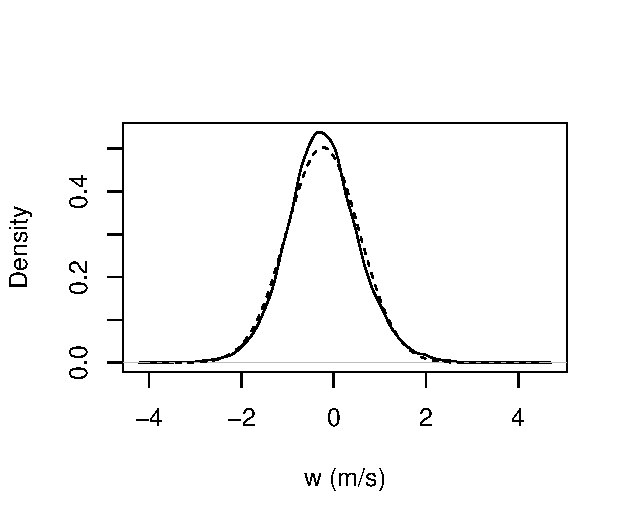
\includegraphics[scale=1.1,keepaspectratio=true]{./diagrams/get_raw_data_1.pdf}
 % get.raw.data.1.pdf: 288x180 pixel, 72dpi, 10.16x6.35 cm, bb=0 0 288 180
 \end{center}
 \caption{Result from first example; normal density (dashed line) shown for reference}
 \label{fig:get.raw.data.1}
\end{figure}

Quantifying data availability in a single file is an often-performed task, to which no SonicLib function has been devoted. The reason is, deciding whether a data item is valid (and then contributing to availability) or not includes a bit of subjectivity. And more important, testing availability within a hourly file is usually very simple, and may be accomplished by directly using R capabilities.

In the next example availability is checked by counting how many data have been labeled ``valid'' by the ultrasonic anemometer, and comparing the result with the total number of (valid and invalid) data lines. The result is expressed in percent form.

\begin{verbatim}
> d <- get.raw.data("../TestData/20100516.10.csv", verbose=TRUE)
> 100 * sum(!is.na(d$data$w)) / length(d$data$w)
  [1] 100
\end{verbatim} 

100\% of data availability within a single hour is quite common with ultrasonic anemometers, thanks to their immunity to  wind calms.

\subsection{Notes}

\begin{itemize}
 \item If optional (e.g. water or carbon dioxide) columns are present they are read with no applied time shift, so that it may be estimated a posteriori if necessary.
 \item All data read are not scaled, all changes necessary to transform from original instrument files and sonic standard raw files having been made previously by adapter procedures, fed with appropriate conversion parameters. 
\end{itemize}


\section{Read Multiple Standard Ultrasonic Anemometer Raw Data Files}
\label{sec:Get Multiple Raw Data Files}

\subsection{Function Use}

To read a single standard ultrasonic anemometer data file use function

\begin{verbatim}
get.multi.raw.data(file.name, n.hours=1, sampling.rate=10,
     threshold=0.005, average.by="none", verbose=FALSE)
\end{verbatim}

\noindent where

\begin{description}
 \item[file.name] is the name of first file to read, according to the specification given in section \ref{sec:FileFormat}.
 \item[n.hours] is the number of hours to stich together (default: 1).
 \item[sampling.rate] is an integer number indicating the sampling rate $f_{s}$ in samples per second adopted when collecting all data in file, according to user knowledge. This value is used to compute the expected number of data in file as $n_{s} = 3600 \cdot f_{s}$; the expected number of data is compared with the number of data actually present in file, $n$ and if the relative difference $(n-n_{s})/n_{s}$ is smaller than a threshold value (see next parameter) the data set is refused. Default = 10.
 \item[threshold] Value of the relative difference $(n-n_{s})/n_{s}$ between actual and expected number of data below which data set is refused. Default = 0.005.
 \item[average.by] String, whose allowed values are ``none'' (default), ``seconds'' and ``minutes''; if ``none'', data are gathered as they are, without any averaging; if ``seconds'', data are averaged on one second basis; if ``minutes'', data are averaged on 1 minute basis.
 \item[verbose] Boolean flag. If TRUE, error and progress message are printed to screen (most useful in interactive use). If FALSE, no message is printed and the success can be assessed only by inspecting output value.
\end{description}

The routine yields a result which on error is NULL (an error message is printed in case only if ``verbose'' parameter is TRUE). If data read has been completed successfully result is an object of type ``sonic.raw.data'', described in \ref{sec:FileFormat}.

\subsection{Examples}

Function \verb|get.multi.raw.data| is typically used in preparation of spectral analysis, when multi-hour files are to be packed together in order to gain band on the left side of log-log diagrams customarily used in micro-meteorology.

The following example shows an example of such a preparation (without the actual spectral part).

\begin{verbatim}
> d <- get.multi.raw.data("../TestData/20100516.00.csv", n.hours=4, verbose=TRUE)
\end{verbatim} 

Proceding this way, and accepting all default, we requested in fact to get four data files and stitch them one after the other, without any averaging (the default value of \verb|average.by| is \verb|"none"|). Operating at 10 Hz this will produce a data set whose length will be around $36000 \cdot 4 = 144000$, quite huge for even the fastest FFT (which if data size is not a power of 2 may degrade performance from order $n \cdot \log n$ to $n^{2}$. More important, the result will be very noisy as information from many frequency scales is all mixed together.

A sensible approach might be to average data every seconds, improving the overall appearance of the low frequency part of spectral diagram, but losing an order of magnitude on the Nyquist frequency (from 5 to 0.5 Hz). The call with per-second averaging is:

\begin{verbatim}
> d <- get.multi.raw.data("../TestData/20100516.00.csv", n.hours=4, average.by="seconds", verbose=TRUE)
\end{verbatim} 

\subsection{Notes}

Function \verb|get.multi.raw.data| is designed to stitch together a \emph{reasonable} number of data files, say from 1 to 8. Averaging is done after all raw data are read and stitched together, even if per-second or per-minute averaging is made. This will result in significant memory occupation if the number of hours to get is high.

For this function to complete successfully it is required that all individual data files exist, and contain at least $100 \cdot (1-\mbox{threshold})$ percent of data. This may seem restrictive (at least if the small default threshold value is retained), but it helps spectral calculations, for which the function has mostly have been written: allowing a high number of gaps would in case force to employ costly periodogram-based algorithms instead of lightweight FFTs. Of course, the authors opinion is just an opinion, and you, the user, are entirely free of choosing your sensible threshold value: you go, gal - at your own risk.


\section{Extract Subset from a Standard Ultrasonic Anemometer Data Set}
\label{sec:Extract Subset from Raw Data Set}


\section{Average Data from a Single Raw Data File}
\label{sec:Average Single Raw Data File}

\subsection{Function Use}

To average data from a single raw data file use this function:

\begin{verbatim}
average.sonic.data(
  d, 
  initial.stamp,
  averaging.time=30,
  delay=0.3,
  trend.removal="none",
  spike.detection.threshold=3,
  spike.treatment="set.na",
  verbose=FALSE
)
\end{verbatim} 

\noindent where

\begin{description}
 \item[d] is an object of type \verb|sonic.raw.data| on which averages are taken.
 \item[initial.stamp] is a POSIXct date and time associated to the beginning instant the data in file have been gathered; this date and time is not arbitrary, and may be generated from file name \emph{in normal cases}. In some circumstances, however, it may be useful to shift time forward or backward by some fixed time, for example to adjust a systematic error of data acquisition system clock. By the way: the POSIXct date and time corresponding to file name may be obtained through function \verb|time.stamp.from.name|, whose use is described later on as an example.
 \item[averaging.time] is a positive integer $t_{a}$, whose admissible values are 10, 15, 20, 30, 60, indicating the averaging time to be used. Default: 30.
 \item[delay] A real number indicating a unique delay value to applied to any optional columns simultaneously, or an object of class ``delay.spec'' indicating the delay used for any possible optional column. Objects of class ``delay.spec'' are created using function \verb|set.delay|, whose use is described in the examples. Default: 0.3 s.
 \item[trend.removal] is a string specifying the trend removal algorithm to use. Possible values are ``none'' (no trend removal is performed), ``linear'' (trend is estimated by linear least squares regression and removed in mean-preserving fashion). The default is ``none''.
 \item[spike.detection.threshold] A real number indicating a unique spike detection threshold to be used for all channels, or a structure of type \verb|spike.detection.threshold| containing the individual thresholds for each channel. All spike detection threshold values are positive numbers meaning a iven number of standard deviations. For example, a value of 2 means "two standard deviations". Default: 3.
 \item[spike.treatment] String, meaning the type of processing to be made on spikes. The possible choices are "none" (no spike processing made, in which case parameter \verb|spike.detection.threshold| is ignored), and "set.na" (spikes are replaced with NA values). Default: "set.na".
 \item[verbose] A boolean flag indicating whether messages are to be printed (TRUE) or not (FALSE).
\end{description}

Function \verb|average.sonic.data| returns on exit a NULL value in case of failure, or an object of class \verb|sonic.avg.data|, described in section \ref{sec:sonic.avg.data}.

\subsection{Time stamps: needed or not in data files?}

Section \ref{sec:sonic.avg.data} lists \verb|time.stamp| among the ``mandatory'' columns. But a word of caution is necessary here, as things are somewhat less dramatic.

In fact: section \ref{sec:sonic.avg.data} deals with the SonicLib raw data files \emph{as they look after they have been read into memory}. This is not exactly the same as how the very same data appear \emph{on disk}.

To date the only difference between SonicLib raw data files on disk and their memory representation is the time stamp, which may be missing from disk files.

In this case, the time stamp is inferred from data using the rule

\begin{equation}\label{eq:Inferred time stamp}
 t = 3600 \cdot \frac{i-1}{n}
\end{equation}

\noindent where $i$ is the data item index and $n$ the total number of data items in file. You may notice from \ref{eq:Inferred time stamp} that time stamp is stored as a number in interval $0 \le t < 3600$.


\subsection{Wind speed: many definitions}

If the concept of wind velocity vector is quite intuitive and inherently unambiguous, the same can not be said of wind \emph{speed}. The reason is, no unique definition exists: a good reason to make a bit of order.

The \emph{three-dimensional speed} is the length of instantaneous wind vector, $U_{3} =\sqrt{u^{2} + v^{2} + w^{2}}$. Its mean value, $\overline{U_{3}}$, represents the full three-dimensional wind speed.

The \emph{horizontal} wind speed is defined in a similar manner than three-dimensional wind, with the two horizontal dimensions only, $U = \sqrt{u^{2} + v^{2}}$. Its mean represents the \emph{scalar velocity}, or wind speed \emph{tout-court}. And here comes the first ambiguity: what horizontal exactly means? In principle the horizontal plane should be the plane perpendicular to local vertical. But in practice it coincides with the \emph{instrumental} horizontal. Instrumental and local horizontal should ideally coincide, but inevitable small errors of positioning prevent this identification to be absolute.

A third type of speed is in common use: \emph{resultant speed}. This is defined as $U_{r} = \sqrt{\overline{u}^{2} + \overline{v}^{2}}$, that is, the length of average horizontal vector. Because of this definition resultant speed can not be larger than scalar speed. The ratio $\frac{U_{r}}{U}$ is always between 0 and 1, the former value being reached when wind sweeps all possible direction with even intensities, and the latter corresponding to a perfectly uni-directional wind.


\subsection{Standard deviation of the wind direction}

The problem of computing the standard deviation of wind direction is not completely defined, as measuring the deviation of an instantaneous direction angle to a mean direction is inherently ambiguous given the modular nature of angles.

Then, instead of computing the standard deviation directly, in literature many estimators have been proposed for estimating it. Among them, Yamartino method is widely acknowledged to provide the better results in a variety of conditions.

Yamartino estimate starts from the instantaneous horizontal wind versors, defined ad

\begin{equation}\label{eq:Horizontal wind versors}
	\mathbf{j} = \left [ u_{j}, v_{j} \right ]
\end{equation}

\noindent where

\begin{equation}
	u_{j} = \frac{u}{\sqrt{u^{2} + v^{2}}}
\end{equation}

\noindent and

\begin{equation}
	v_{j} = \frac{v}{\sqrt{u^{2} + v^{2}}}
\end{equation}

\noindent with $u$ and $v$ the two horizontal wind components along directions $x$ and $y$.

Once the instantaneous versors have been computed, their components average is taken, $\overline{u_{j}}$ and $\overline{v_{j}}$, and the quantity

\begin{equation}\label{eq:Yamartino epsilon}
	\varepsilon = \sqrt{1 - \left( \overline{u_{j}}^{2} + \overline{v_{j}}^{2} \right)}
\end{equation}

\noindent is then computed. The standard deviation of wind direction is finally estimated as

\begin{equation}\label{eq:Yamartino estimate of standard deviation of horizontal direction}
	\hat{\sigma_{A}} = \left( 1 + \alpha \varepsilon^{3} \right)\cdot \arcsin{\varepsilon}
\end{equation}

\noindent where $\alpha = \left( \frac{2}{\sqrt{3}} - 1 \right)$.


\subsection{Trend removal}

One common manifestation on non-stationarity in data is the occurrence of a slow variation in data, as if their mean value drifts following some smooth function of time.

This slow variation is visible within any averaging interval, and may be approximated by a linear function.

As we're using time averages and covariances within each averaging block, if this slow variation is not removed its value will leak into covariances, and appear as a fictive turbulent flux.

It is worth noticing the adverse effects of linear trend are a direct consequence of the way we compute the means and covariances as basically time averages. For them to make sense in the context of data processing of sonic anemometer measurements it is necessary that time averages and ensemble means coincide, which is possible only if we assume stationarity in the process underlying data, and in data themselves. The presence of a linear trend directly invalidates this assumption and, with it, any further serious consideration.

The problem then arises, on how to remove linear trends from any averaging block in sonic data series.

One solution assumes data are positioned in time with sufficient precision. Then, we may take all couples $(t_{i},s_{i})$, where $s$ indicates signal values and $t_{i}$ the corresponding time instant, and treat them as experimental points. Them given, we want to identify the corresponding linear model

\begin{equation}\label{eq:Trend Concept}
 s = a \cdot t + b + \varepsilon
\end{equation}

\noindent where $\varepsilon$ is a model error.

One popular way to identify model (\ref{eq:Trend Concept}) is by minimizing the squared difference between experimental points and model values at the corresponding instant. This linear least squares regression yields the equation of a line $s(t) = a \cdot t + b$ which is an estimate of our trend.

Now, if we limit to subtract the trend estimate from the original signal, we obtain

\begin{equation}\label{eq:Mean changing trend removal}
 S_{i} = s_{i} - a \cdot t_{i} - b
\end{equation}

noindent whose average is

\begin{equation}
 \overline{S} = \frac{1}{n} \sum_{i=1}^{n} S_{i} = \frac{1}{n} \sum_{i=1}^{n} s_{i} - a \cdot \frac{1}{n} \sum_{i=1}^{n} t_{i} - b = \overline{s} - a \cdot \overline{t} - b
\end{equation}

\noindent which is not the original $\overline{s}$, nor in general has some desirable property as being zero. So, within SonicLib liner trend removal is \emph{mean-preserving}: after the linear trend has been removed using (\ref{eq:Mean changing trend removal}) the new signal mean is computed and subtracted from the transformed signal. Then, the mean of original signal is added back. In other terms:

\begin{equation}\label{eq:Mean preserving trend removal}
 S_{i} = s_{i} - a \cdot t_{i} - b - \overline{S} + \overline{s}
\end{equation}

Changing the trend-freed signal so that its mean is preserved has no effect on covariances, meanwhile allowing to perform average-depending computations (for example finding rotation angles in eddy covariance).

For all this to be possible, however, we need each data item is accompanied by a non-ambiguous time stamp $t_{i}$ In section \ref{sec:SonicLib Raw File Time Stamps} we have seen this is not necessarily the case: all we may be reasonably sure is time stamps are ``regular''.

Time stamp regularity is just fine if all we need to do is partitioning a signal collected in an hourly file among various averaging blocks. But regrettably it is not sufficient to compose experimental points suitable to linear regression. As a workaround, and only for trend removal, an equally-spaced time stamp is synthetized from index by applying the following rule:

\begin{equation}
  t_{i} = \delta t \cdot (i-1)
\end{equation}

\noindent where $\delta t = 1 / f_{s}$.

It is worth mentioning this trend removal strategy is effective only when trend originates from a smooth change as temperature's normal daily variation. It is completely worthless in cases where the trend takes for example the form of a sudden change, like when a cold or warm front breaks in, or at beginning of Foehn episode.

Another more subtle point is that trend removal as done in SonicLib is entirely ``statistical'': it is always possible to perform it, but it has no ``real'' physical meanings. The trend a human eye and brain can detect, however, are of entirely physical origin. An ideal trend removal strategy should take this into proper account. In SonicLib, at least in the moment, we don't.

\subsection{Spike detection and processing}

In ultrasonic anemometry lingo, the term \emph{spike} is used as a synonym of outlier in a data series. So the question arises on agreeing on what an "outlier" actually is - which also answers, at least in part, to the question on what is the most appropriate way of detecting them.

In the practice of statistics outliers are often intended as individual data whose values are not compatible with the distribution underlying the whole data set (outliers excluded). In other terms, it is assumed a data set always contains a subset which is drawn from some well known distribution (not necessarily normal), plus a few number of data whose value has been perturbed during the collection process.

The nature of this perturbation is left unspecified. But of course, its occurrence is sufficient to make that individual reading "something else" than the real data. Think, for instance, to a glitch in an analog to digital converter due to an electric power outage (maybe a brown-out": it's a rare event (which indeed \emph{may} occur), whose most likely event is to alter the original reading imparting it a random deviation.

In strict principle the random deviation imparted by the measurement glitch is not guaranteed to be large: in many cases it is indeed small enough that its effect remains undetected. But on occasions it may result in a change so macroscopic that we can detect it easily. In this case, we have an outlier.

Assuming outliers exist is prudential in ultrasonic anemometry, even for sonics performing plausibility checking on individual data. Reasons for them abound, from electrical noise to alterations (e.g. rain drops) along the measurement path. Although rare, it is highly unlikely all of these events will be detected without error by an automatic method which is (at least with current electronic technology) performed on individual data without taking into account the past values history.

This, indeed, lifts the veil on what outliers are in practical sense: their nature is highly contextual. If you plot your data set in the time domain, outliers emerge as spikes on the plot. But if your sight is restricted to only one data item, then you have little to base your detection on, apart from some quite indirect indicators like for example an imbalance in the attenuation between direct and opposite sound pulse propagation paths.

And, yes: its very name reveals that spikes are a highly \emph{visual} concept. Usually, translating visually obvious concepts into mathematical concepts is a hard nightmare. The human eye took billion years of random variation and natural selection to perfection. And the neural circuitry within of it and beyond, in the brain, is way more complex and powerful than any computer. It is very hard to simulate what we gut-feel as "visually obvious" using a piece of software, when simulating the behavior of a \emph{single} neuron with sufficient accuracy requires a multiprocessor supercomputer (and the simulation proceeds slower than a normal neuron can operate). Really, there is no hope to reproduce visual feeling.

But, we can often find approximate methods. This is what happens with outliers. The most popular way of detecting them is by looking for data values which do \emph{not} satisfy the condition

\begin{equation}\label{eq:Common outlier detection method}
	q_{\epsilon} \le x \le q_{1-\epsilon}
\end{equation}

\noindent where $q_{u}$ is $u$-th quantile drawn from the distribution underlying our data set. As this distribution is a priori unknown, quantiles from the data set itself are often used in practice. By doing so, we can see how "detecting outliers" actually means "discarding the lower and upper tails of the data set": not exactly the same thing, but practically sufficient in most cases.

Computing quantiles, unfortunately, demands much more work than calculating a mean and standard deviation. In practice you have to sort data, if you want to locate the smaller and the larger, and this is an $O(n \log n)$ operation, quite heavier than the $O(n)$ order of mean and standard deviation computations. This may not be a real challenge with today's computers, but it was decidedly not when ultrasonic anemometry began in the late seventies of past century.

The desire to locate spikes in real time then suggested to adopt a spike detection criterion of quite simplified nature, like this:

\begin{equation}\label{eq:Actual spike detection method}
	\mu - K \sigma \le x \le \mu + K \sigma
\end{equation}

\noindent where $\mu$ and $\sigma$ are mean and standard deviation of data set respectively, and $K$ a real positive constant, one of whose most popular values is 3. Still today, by ingrained habit, this is the way spikes are detected in ultrasonic anemometry, and SonicLib adopts it instead of quantile-based method.

We notice one macroscopic thing: the fact of not satisfying (\ref{Actual spike detection method}) is equivalent to (\ref{eq:Common outlier detection method}) \emph{only if the underlying distribution is normal}. But this assumption is not necessarily true for experimental data! (This is a plain understatement: for sonic anemometer data sets it is plainly false). So, what to say? Fortunately, as often happens with practical statistics, the approximation we get is not that bad, so detecting outliers the wrong ways indeed works (with an accuracy sufficient to prevent losing our sleep).

There is another thing to say about spike detection, and it is a macroscopic one: \emph{of course}, for it to make sense, the data set must be \emph{stationary}. Would it not be, for example because of a linear trend, then standard deviation (or quantiles, for what matters) would inflate and finding just one outlier would become really a challenge. Think looking for the classical needle in a haystack ten times the size of a normal one.

That is to say, spike detection must be performed \emph{after} trend removal!

Of course, we have to take into account a practical (unavoidable) difficulty: trend removal is based on finding a regression line, a process which is notoriously sensitive to outliers (which in the moment of trend identification are still there). The trend may then be located with some error, whose occurrence would likely have the effect of widening our fishing net somewhat.

To overcome this difficulty we could proceed iteratively, by re-fitting trend after spike have been treated in some way. In SonicLib, as in most practical implementations, this is \emph{not} made, mainly to save computing time.

Now: what to do of the sppikes we have detected? In principle we could do many things. One method we can use is to say "OK, my ultrasonic anemometer performs a lovely plausibility checking on individual data, and I have no specific reason to not believe it". This head-in-the-sand approach may look dangerously akin to "managing by absence", but on some occasions may not be entirely without any sense.

Another possible approach is to shave spikes off in some way. A popular method is replacing their values by the linear interpolant of data immediately before and after. But: who guarantees that the real data would have been this way? Indeed, this method is very attractive as it does not increase the number of "invalid" data. This could make computations a bit easier to implement for programmers, at the price of introducing into data some degree of poetical invention. The same would indeed happen if we adopt any other, less crude, data imputation method.

Last, we may just suppress spikes by replacing them with NAs. In \verb|R| this is no problem at all, as the language already includes the ability to get rid of invalid data when computing means and (co)variances (for example by \verb|is.na=TRUE| key). This is the approach followed in SonicLib.

It is worth mentioning, in the interest of preventing a next little religion war, that replacing spikes with valid, although more domestic, data or killing them does not alter significantly the end results: by definition, spikes are "few"! One consequence of the "killing" approach is, we will not be able to use FFT based spectrum calculation if even one spike is found. But this is not a big deal for SonicLib: we may adopt in this case power spectrum estimation instead. Or, if we know our anemometer plausibility checks are acceptably sound, even choose to adopt the "head in the sand" approach and hope for the best.

\subsection{Examples}
\subsubsection{Simple data averaging}

In many cases all what done is just averaging data the simple way, accepting all defaults. This is accomplished by issuing a sequence like this:

\begin{verbatim}
> file.name <- "../TestData/20100516.10.csv"
> d <- get.raw.data(file.name, verbose=TRUE)
> d.stat <- average.sonic.data(d, time.stamp.from.name(file.name))
\end{verbatim} 

Result, stored in variable \verb|d.stat|, contains one record per each of the two 30 minutes block within hour.

\subsubsection{Using different delays for different variables}

When more than one analog data set is in raw data file it may happen their data acquisition delays to differ. If this is the case, a unique real valued delay (like the default value) cannot be used, and function \verb|set.delay| is to be used.

The following example shows how different delays are used, assuming a LiCor 7500 water and carbon dioxide detector and a Vaisala HMP45 thermo-hygrometer are connected to ultrasonic anemometer's analog input channels (and then, available in files):

\begin{verbatim}
> dly <- set.delay(q=0.3, c=0.3, temp=0.0, hrel=0.0)
> file.name <- "../TestData/20120401.03.csv"
> d <- get.raw.data(file.name, verbose=TRUE)
> d.stat <- average.sonic.data(d, time.stamp.from.name(file.name),
                delay=dly)
\end{verbatim} 


\subsection{Notes}

Function \verb|average.sonic.data| is seldom used directly, as most data processing occurs on entire campaigns more than a unique file. It may however happen access to data in a single hour is needed (maybe for diagnostic purposes), and then it makes sense to use \verb|average.sonic.data| on its own.

Averages and covariances are computed according to the usual definitions, that is blockwise. No weighting nor pre-filtering strategy is employed during averaging (although signal preparation may have been made priori of this step).

The relative non-stationarity of wind component $x$ is defined as

\begin{equation}\label{eq:Relative Nonstationarity of X}
 RN_{x} \doteq \frac{\delta x}{\overline{x}}
\end{equation} 

\noindent as defined in \cite{Vickers1997}. Non-steadiness of covariance $\overline{x'y'}$ is defined according to \cite{Foken1996} as

\begin{equation}\label{eq:Non Steadiness of xy}
 NS_{\overline{x'y'}} \doteq \frac{\hat{x'y'} - \overline{x'y'}}{\overline{x'y'}}
\end{equation} 

\noindent where

\begin{equation}\label{eq:Partial Covariance}
 \hat{x'y'} \doteq \frac{1}{n} \sum_{i=1}^{n}\overline{x'y'}_i
\end{equation} 

The symbol $\overline{x'y'}_i$ designates the \emph{i}-th 5 minutes block within averaging time. $n$, the number of blocks, may be computed readily as $\frac{t_{a}}{5}$, where $t_{a}$ represents the averaging time in minutes. Note $n$ is an integer, because of the restrictions imposed on allowed values of $t_{a}$.


\section{Average Data from Multiple Raw Data Files}
\label{sec:Average Multiple Raw Data Files}

\subsection{Function Use}

Computing averages is most often done on the result of whole measurement campaigns. If these are stored in a single file, then averaging may be performed using function

\begin{verbatim}
average.sonic.file.set(
  dir.name=".",
  time.zone="UTC",
  shift=0,
  averaging.time=30,
  sampling.rate=10,
  threshold=0.1,
  delay=0.3,
  trend.removal="none",
  spike.detection.threshold=3,
  spike.treatment="set.na",
  verbose=FALSE
)
\end{verbatim} 

\noindent with the following argument meaning:

\begin{description}
 \item[dir.name] Name of directry where data are looked for (default: current directory).
 \item[time.zone] String containing the standard name of the time zone to which all time stamps will be attributed (default: ``UTC''). 
 \item[shift] Number of seconds to be added to time stamps to obtain ``true'' time, used when mass-adjusting a data set (default: 0).
 \item[averaging.time] Value of averaging time to be used when processing data in set, in minutes (default: 30; allowed values: 10, 15, 20, 30, 60).
 \item[sampling.rate] Sampling rate assumed for data in set, in Hertz (default: 10).
 \item[threshold] Fraction of missing or invalid data above which an averages record is considered statistically invalid, and assigned the NA value (default: 0.1).
 \item[delay] A real number indicating a unique delay value to applied to any optional columns simultaneously, or an object of class ``delay.spec'' indicating the delay used for any possible optional column. Objects of class ``delay.spec'' are created using function \verb|set.delay|, whose use is described in an examples of section \ref{sec:Average Single Raw Data File}. Default: 0.3 s.
 \item[trend.removal] is a string specifying the trend removal algorithm to use. Possible values are ``none'' (no trend removal is performed), ``linear'' (trend is estimated by linear least squares regression and removed in mean-preserving fashion). The default is ``none''.
 \item[spike.detection.threshold] A real number indicating a unique spike detection threshold to be used for all channels, or a structure of type \verb|spike.detection.threshold| containing the individual thresholds for each channel. All spike detection threshold values are positive numbers meaning a iven number of standard deviations. For example, a value of 2 means "two standard deviations". Default: 3.
 \item[spike.treatment] String, meaning the type of processing to be made on spikes. The possible choices are "none" (no spike processing made, in which case parameter \verb|spike.detection.threshold| is ignored), and "set.na" (spikes are replaced with NA values). Default: "set.na".
 \item[verbose] Boolean flag indicating whether output messages should be printed (TRUE) or not (FALSE).
\end{description}

In case of failure a NULL value is returned.

If averaging terminated correctly then an object of class \verb|sonic.avg.data| is returned (see section \ref{sec:sonic.avg.data}).

\subsection{Troubleshooting hints}

Function \verb|average.sonic.file.set| is most likely your first contact with SonicLib: most of processing aimed at ``distilling information from sonic data'' starts from averaging out a data set, and this in turn involves one or more calls to \verb|average.sonic.file.set| as the very first step.

Unfortunately, \verb|average.sonic.file.set| is also quite a delicate step. In itself is not so dramatically difficult from, say, a mathematical or computer science standpoint. But on the other side, it interfaces with ``standard SonicLib raw data files'', the product of a heterogeneous set of converters in quick evolution.

Chances are non-zero that the last minute version of that new shiny converter does not really produce so ``standard'' SonicLib raw data files. This is something the kernel SonicLib and its developers can not directly control, converters often coming from end users.

In cases like these \verb|average.sonic.file.set| stops on error. If parameter \verb|verbose| is set to \verb|TRUE| messages are printed in case of troubles: they may be illuminating but understanding them is much quicker with a little bit of a-priori information.

In the subsections following each of the important error messages is described in its meanings. Before to proceed, we note messages may come from \verb|averaging.sonic.file.set|, \verb|averaging.sonic.file| and \verb|get_raw_data|, that is the function described here and the functions it calls in turn: in the first case the error is likely to reside in something pertaining the file set as a whole, while in the others some specific error on a single data file has occurred (in fact, all messages but one come from the single file command \verb|averaging.sonic.file|).

\subsubsection{Message average.sonic.file.set:: Error: No CSV files in directory}

SonicLib raw data files are CSV file, and their extension must be ``.csv''. If the data directory contains no file with ``.csv'' extension then there is no point for \verb|averaging.sonic.file.set| to do anything.

The most likely cause of this message is you have specified a wrong directory name. This may be because the directory does not exist, or it exists but really contains no CSV file.

Notice that if at least a CSV file exists as far as \verb|averaging.sonic.file.set| is concerned it's all right. The message is not emitted and, as soon as \verb|averaging.sonic.file.set| will try reading the wrong CSV file some other error will occur.


\subsubsection{Message average.sonic.data:: error: Argument 'delay' is not a member of an instance of class ``delay.spec``}

This message means you have specified a delay of the ''wrong type``. Delays, used to cope with the small retard analog data sampled from sensors connected to ultrasonic anemometers often exhibit, can be only numbers (in which case the same delay value is applied uniformly to all channels), or lists of class ''delay.spec``).

Anything else would make \verb|averaging.sonic.file.set| quite hysterical; to avoid this possibility a type check is made and in case of failure the message is printed.

If you see this message just check parameter \verb|delay|.

\subsubsection{Messages average.sonic.data:: error: Averaging time is not a multiple of 5 minutes, average.sonic.data:: error: Averaging time is not a divisor of 60 minutes, Message average.sonic.data:: error: Averaging time is not between 10 and 60 minutes}

All these messages are self-explaining: averaging time must be a multiple of 5 minutes dividing exactly one hour and not smaller than 10 minutes.

In practice, the values allowed for the averaging time are 10, 15, 20, 30 and 60 minutes.

If the value of the averaging time is set to a number not satisfying any of these conditions one of the messages is emitted.

\subsubsection{Message get.raw.data:: Error: No columns in input data}

This message basically tells SonicLib did not understand what the content of a file is.

The most common reason is the file is not a SonicLib raw data file, although its type is CSV. From a purely technical standpoint this may mean the file has been prepared using a spreadsheet and exporting to CSV, but the original file did not contain tabular data.

In practice, the meanings is the directory assumed to contain only SonicLib raw data also contains something else, and of a very strange nature.

An important thing to notice is that despite of the ''error`` nature of this message the function \verb|averaging.sonic.file.set| does not stop upon encountering it: the offending file is just skipped and nothing bad happens (apart from the message).

Anyway, if this error annoys you the best you can do is moving the wrong file somewhere else. Locating it is quite simple: before printing the error message SonicLib dumps the name of the current file to the R concole.

It is not unworthy to stress that SonicLib expects the directory containing raw data files is ''clean``, that is, contains nothing different than SonicLib raw data files.

\subsubsection{Message get.raw.data:: Error: Number of data inconsistent with the expected number}

This message in practice tells SonicLib was able to find something tabular in a data file, but the number of rows does not match with the expected number.

This latter is assumed equal to $n_{s} \doteq f_{s} \cdot 3600$, where $f_{s}$ is the sonic's data acquisition frequency employed when collecting current data file. Given $n$, the number of data records actually present in file, the following indicator is formed:

\begin{equation}\label{eq:F indicator}
  F = \frac{\left| n - n_{s} \right|}{n_{s}} - 1
\end{equation}

If $F$ is smaller than the threshold, the corresponding data file is rejected. $F$ represents the deviation of total data in file from the number of expected data, expressed in fraction form. Because of the absolute value in \ref{eq:F indicator} the check operates both when the number of actual data is smaller than expected, and when it's \emph{larger}. This choice allows to trigger attention on data sets whose acquisition parameters differ from the ones assumed, which in many cases are just left to their default values: if this message occurs on any file in the data set, then you may be sure the assumed sampling frequency is wrong.

Assigning a sensible value to the threshold may involve contextual data. As a general rule, however, a tighter threshold might make sense when averaging and trend removal are made, or when an averaging period of less than an hour is adopted (regardless on trend removal state). The default in \verb|averaging.sonic.file.set|, 0.05, reflects this.

\subsubsection{Message get.raw.data:: Error: No 'u', 'v', 'w' or 't' data in file}

This message tells that at least one of the mandatory columns expected in a SonicLib file is not present, and as a consequence the file is rejected.

A likely cause of this error is the supposed SonicLib raw data file is not really a SonicLib file. Or, the column names within of it are wrong (this \emph{may} happen: SonicLib raw data file columns are spelled in lowercase, and maybe the converter wrote them in uppercase).

It's interesting to note the time stamp is not mentioned in this message. The reason is, time stamp is generated automatically if missing from data files. But: for this approach to make sense the file must be reasonably free from gaps, that is, $F$ must be smaller than the (tight) threshold.

\subsection{Examples}
\subsubsection{Averaging data ``acritically''}

Function \verb|average.sonic.file.set| may be used to just load data and average them on the fly, maybe within an automatic offline data processing script like in this example:

\begin{verbatim}
d <- average.sonic.file.set(
  "../TestData",
  delay=0.3, verbose=FALSE
)
\end{verbatim} 

\subsubsection{Preliminary assessment of data quality}

The result of preceding call may then be used directly to feed data processing functions like \verb|eddy.covariance|, as will commonly be made by many users (and automatic procedures).

But if we desire, we can do some more: use averaging and its associated calculation of relative nonstationarity and non-steadiness indices as a direct exploratory tool to preliminarily assess data quality.

In the next example we use averaging to check which hourly files are affected by significant non-stationarity on wind component $w$ and sonic temperature $theta$.

This makes sense if we desire to compute turbulent heat flux from sonic anemometer data reliably, and we can afford the risk of rejecting low-quality data sets.

Of course things are not everytimes this lucky way. For example, if our objective is to feed a lagrangian dispersion model in real time then it could make better sense to be less finicky with data, and accept hours characterized by a sub-standard quality: in cases like this it may be better to use available measurements, accepting the risk some of them are not ``scientific paper strength'', instead of resorting to data imputation strategies (that is, invention of fictive but ``plausible'' data to fill gaps). As almost always happens with data processing, the ``best'' way depends very much on the context.

So, let's assume we want to collect the subset of data on which e.g. eddy covariance will likely get best results, maybe in view of a scientific publication. Because of the assumptions underlying eddy covariance, results tend to be better when data are ``stationary''.

In a real data set, however, stationarity will never be really fulfilled. The requirement of stationarity is simply too restrictive, and no natural data set will lack its part of trends, changes (often abrupt) of variance or covariance, and infinite more.

So pragmatically we define a hourly file to be ``stationary enough'' if relative non-stationarity of $w$ is, say, less than 0.5 and the non-steadiness of $\overline{w'\theta'}$ less than 0.3.

Our first step is averaging data. But as we're interested in assessing quality of \emph{hourly} files we avoid using the default of \verb|averaging.time|, 30 minutes, and specify 60 minutes instead:

\begin{verbatim}
d <- average.sonic.file.set(
  "../TestData", averaging.time=60,
  delay=0.3, verbose=FALSE
)
\end{verbatim} 

\noindent Actual plotting may then be made with standard R commands, like this:

\begin{verbatim}
plot(
  d$data$t.stamp,
  d$data$w.avg,
  xlab="",
  ylab="Non-rotated W (m/s)",
  main="",
  type="l"
)
\end{verbatim} 

Here incidentally we see how convenient it is having adopted R for developing SonicLib: in addition to SonicLib specific function (in fact, a tiny set), we gain access to the immense graphic and data analysis facilities already built into R.

Taking this for granted, we may then plot the time evolution of relative non-stationarity and non-steadiness we're interested in, along with the corresponding limiting values we've selected so far. The result is shown in figures \ref{fig:average.sonic.file.set.1} and \ref{fig:average.sonic.file.set.2}.

But before of this we may do a simpler check, directly on available data. In our case we may learn quite a bit just plotting the hourly averages of vertical wind velocity. The importance of this and other similar ``simple'' checks can not be overlooked: in our specific case, finding a significantly non-zero vertical mean before applying axis rotation may indicate some positioning problem, and more so if all values have the same sign, thus indicating some systematic trouble.

In our data set, ``CRA.01'', this is precisely what happens, as we may see in figure \ref{fig:average.sonic.file.set.0} where we see all non-rotated hourly means of vertical speed to be negative, and indeed quite large. Why does this happen? Is this related to some specific provenance direction, or happens in all cases? Answering these and other related questions is fundamental when documenting micro-meteorological campaigns, and often involves both describing site conditions and performing exploratory data processing before embarking in the huge processing work.

\begin{figure}[htp]
 \centering
 \begin{center}
 \includegraphics[scale=1.1,keepaspectratio=true]{./diagrams/average_sonic_file_set_0.pdf}
 % average.sonic.file.set.1.pdf: 288x180 pixel, 72dpi, 10.16x6.35 cm, bb=0 0 288 180
 \end{center}
 \caption{Time evolution of hourly-averaged wind component $w$ in data set ``CRA.01''}
 \label{fig:average.sonic.file.set.0}
\end{figure}

\begin{figure}[htp]
 \centering
 \begin{center}
 \includegraphics[scale=1.1,keepaspectratio=true]{./diagrams/average_sonic_file_set_1.pdf}
 % average.sonic.file.set.1.pdf: 288x180 pixel, 72dpi, 10.16x6.35 cm, bb=0 0 288 180
 \end{center}
 \caption{Time evolution of relative non-stationarity of wind component $w$ in data set ``CRA.01''; note the threshold value is negative, as all averages of $w$ are lower than 0 in the test data set considered}
 \label{fig:average.sonic.file.set.1}
\end{figure}

\begin{figure}[htp]
 \centering
 \begin{center}
 \includegraphics[scale=1.1,keepaspectratio=true]{./diagrams/average_sonic_file_set_2.pdf}
 % average.sonic.file.set.2.pdf: 288x180 pixel, 72dpi, 10.16x6.35 cm, bb=0 0 288 180
 \end{center}
 \caption{Time evolution of non steadiness of covariance $\overline{w'\theta'}$ in data set ``CRA.01''}
 \label{fig:average.sonic.file.set.2}
\end{figure}

As we may see from figures \ref{fig:average.sonic.file.set.1} and \ref{fig:average.sonic.file.set.2}, most hours are ``good'' (in the strict sense that both relative non-stationarity of $w$ and non-steadiness of $\overline{w'\theta'}$ are below their respective thresholds. But some cases exist when one or both of these diagnostic values exceed the threshold.

What to do in these cases?

As mentioned before, no best a priori method can be devised, and a sensible answer must take the overall context into proper account. If, as we imagined, the purpose of the measurement campaign is to write a scientific paper stating some new truth, then it may make sense to \emph{exclude} from any further use the hours whose non stationarity or non steadiness exceed their thrsholds.

Space restrictions do not allow us to proceed further, but an analysis might be worth on rejected data to see whether they really \emph{are} non-stationary. And if so, \emph{why}. Exceptions in data are very often revealing of something deep and unexpected, and it would be a little pity having to just not use them. These detailed analyses, in any case, are highly exploratory and visual, and here R really shines as a life-saving helper.


\subsection{Notes}

Function \verb|average.sonic.file.set| assumes argument \verb|dir.name| to specify a directory in which data files in standard SonicLib format are found, but this does not mean they are required to be unique, nor that some of them are completely missing.

To avoid confusion however it is highly recommended to avoid placing in the data directory anything different from data, and to separate data from different campaigns in different directories. Function \verb|average.sonic.file.set| continues to operate normally in these cases, but results are homogeneous and without strange surprises - at least, strangeness stems from data themselves.

%*************************************************************************
\chapter{Analyzing Data}
\label{chap:Data Analysis}

\section{Spectral Analysis}
\label{sec:Spectral_Analysis}

\section{Multiresolution Analysis}
\label{sec:Multires_Analysis}

Multi-resolution (or "multi-scale" - in this Manual we consider the two terms as synonyms) analysis is performed invoking the following function:

\begin{verbatim}
multires(t.stamp, val, steps)
\end{verbatim}

\noindent where

\begin{description}
\item[t.stamp] Vector, containing time stamps expressed in seconds, as in SonicLib raw data files
\item[val] Vector, the same length of \verb|t.stamp|, containing the values to be analyzed
\item[steps] Vector containing a sequence of strictly decreasing numbers with the property that its $i$-th term is an exact multiple of $i+1$-th.
\end{description}

\subsection{Background}

The idea of applying multi-scale analysis to data sets is far from new. An example can be found in \cite{Percival2000}, which investigates the used of wavelets in statistics. Numerous works have been published on the related subject of multiscale modeling (see \cite{Barth2002}, \cite{Ferreira2007}, and in the specific context of ultrasonic anemometry \cite{Howell1997}).

Three-axial ultrasonic anemometers capture instantaneous samples of the wind vector $\mathbf{v} = [u,v,w]$, temperature $T$ and zero or more analog input values at rates exceeding 40Hz. In principle samples can be positioned precisely in time by means of a time stamp $t$. We may then treat sequences of consecutive samples as time series.

Let's now consider samples taken on a given hour. We may imagine their time stamps to form the sequence

\begin{equation}\label{eq:Time Stamps}
\left\{t_{k}\right\}_{k=1}^{n}
\end{equation}

\noindent where

\begin{equation}
t_{k} = t_{0} + (k-1) \cdot \delta t
\end{equation}

\noindent with $t_{0}$ the hour's initial instant and $\delta t = \frac{1}{f_{s}}$ the sampling period, reciprocal of sampling rate. Similarly we may introduce the sequences

\begin{equation}\label{eq:Wind Vector}
\left\{\mathbf{v}_{k}\right\}_{k=1}^{n} = \left\{[u_{k}, v_{k}, w_{k}]\right\}_{k=1}^{n}
\end{equation}

\noindent of wind vector values,

\begin{equation}\label{eq:Temperature}
\left\{T_{k}\right\}_{k=1}^{n}
\end{equation}

\noindent of temperature and of analog values, if any.

\subsection{Multi-scale decomposition of a time-stamped data sequence}
\label{sec:Multi-scale decomposition}

\subsubsection{Timed sequences}

Forgive me in advance for the nitty-gritty microscopic details which follow. My only justification is, they are quite unavoidable: in what is about to follow, precision is essential to get not lost. (If you still find me quite pedantic, OK, we'll make both a reason! By the way, this is not how I speak normally.)

So let's first take a generic \emph{timed sequence}, that is a collection of generic data values, each associated to its time stamp,

\begin{equation}\label{eq:Timed sequence}
	X = \left\{(t_{k},x_{k})\right\}_{k=1}^{n}
\end{equation}

\noindent under condition $t_{k} < t_{k+1}$. The $t_{k}$ represent \emph{time stamps}, and $x_{k}$ the \emph{values}. A \emph{timed subsequance} of a timed sequence $X$ is a timed sequence

\begin{equation}\label{eq:Timed subsequence}
	Y = \left\{(t_{k_{j}},x_{k_{j}})\right\}_{j=1}^{h}
\end{equation}

\noindent with the ordered couples $(t_{k_{j}},x_{k_{j}})$ chosen in $X$, and such that $t_{k_{j}} < t_{k_{j+1}}$. When $Y$ is a timed subsequence of $X$ we write $Y \dashv X$.

Time stamps of a timed subsequences need not a priori being consecutive, but when they are we have the important case of \emph{proper timed subsequences}. A proper timed subsequence of $X$ is a timed subsequence $Y$ in which $k_{j} + 1 = k_{j+1}$. If $Y$ is a proper timed subsequence of $X$ we write $Y \prec X$. Clearly, $Y \prec X \rightarrow Y \dashv X$.

If $X = \left\{(t_{k},x_{k})\right\}_{k=1}^{n}$ is a timed sequence, by its \emph{time sequence} we intend the sequence

\begin{equation}\label{eq:Time sequence}
	T(X) = \left\{t_{k}\right\}_{k=1}^{n}
\end{equation}

We may figure $T()$ as an operator acting on timed sequences and extracting the time part from them. In a very sense, operator $T()$ is a projection from the "space" (?) of timed sequences to that of ordinary finite sequences in the real field. But OK, this is not really necessary to our (after all very simple) needs, so let this mention stay just as a curiosity. We'll use it anytime useful, without overcommitment.

Two timed sequences $X_{1}$, $X_{2}$ are \emph{time-disjoint} (or simply \emph{disjoint}) if

\begin{equation}\label{eq:Time disjoint timed sequences}
	T(X_{1}) \cap T(X_{21}) = \emptyset
\end{equation}

\noindent that is, if their respective time sequences have no time instants in common. When two timed sequences $X_{1}$, $X_{2}$ are disjoint it makes sense to define their \emph{merge} $X_{1} \oplus X_{2}$ as the time sequence consisting of all couples $(t,x)$ from either timed sequences, ordered with respect to time the usual way.

If $X = X_{1} \oplus X_{2}$, then $X_{1} \dashv X$ and $X_{2} \dashv X$. Nothing dramatic: just another way to say the same thing. It is much more interesting to our case when $X = X_{1} \oplus X_{2}$ with $X_{1} \prec X$ and $X_{2} \prec X$, that is when the two timed sequences contributing to the merge are each proper timed subsequences of $X$. In this case, by necessity, either all time values of $X_{1}$ precede all time values of $X_{2}$, or all time values of $X_{2}$ precede all time values of $X_{1}$. When this happens we can say of a \emph{proper} merge.

This leads us to the important concept of \emph{partition} of a timed sequence $X$. We may define it as a set $\left\{X_{1}, X_{2}, \ldots, X_{p}\right\}$ such that $X = X_{1} \oplus X_{2} \oplus \ldots \oplus X_{p}$. The partition is \emph{proper} if $X_{i} \prec X$ for $i = 1, 2, \ldots, p$.

Last, it is worth introducing a symbol to say all times in a timed sequence $X_{1}$ precede all times in sequence $X_{2}$: we may say $X_{1}$ \emph{precedes} $X_{2}$, or $X_{1} < X_{2}$. This concept of precedence allows us to establish a convention which simplifies all further steps: whenever we have a proper partition of $X$, $\left\{X_{1}, X_{2}, \ldots, X_{p}\right\}$, we assume $X_{1} < X_{2} < \ldots < X_{p}$.


\subsubsection{Interval induced partitions}

Imagine $E$ is a subset of the real line such that $T(X) \subset E$ If we chose wisely, we may get an $E$ of finite length (sure we could chose an infinite length interval $E$: but it would give us no special advantage). Now, let $F \subset E$. We can say the timed subsequence $Y$ of $X$ is \emph{induced by F} if all the elements of $T(Y)$ are "inside" of $F$ and not elsewhere in $E$, that is, $T(Y) \subset F$ and $T(Y) \cap E \setminus F = \emptyset$. When this happens we can write $Y = X_{F}$.

If we don't specify how $F$ is made, then we leave the door open to it having a lot of holes, so that all we can say is $Y \dashv X$. But if $F$ is an interval, then by necessity $Y \prec X$: this, for us, is the interesting case.

Now, let's consider a partition $\left\{F_{1}, F_{2}, \ldots, F_{p}\right\}$ of the interval $E$ in intervals $F_{i}$ (that is, a collection of intervals which are mutually disjoint and whose union coincides with $E$). Its corresponding \emph{induced proper partition} of $X$ is $\left\{X_{F_{1}}, X_{F_{2}}, \ldots, X_{F_{p}}\right\}$.

Partitioning the time axis in equal length intervals and using them to slice a timed sequence is, as we'll see in the next section, the key idea of the kind of multiscale analysis we'll see in this work.


\subsubsection{Temporal scales and temporal scales sequences}

From now on we begin being practical. Consistently with SonicLib way of storing data file, we can imagine $E$ to span exactly an hour starting at instant $t_{0}$, that is, reasoning in seconds,

\begin{equation}\label{eq:An hour}
	E = \left\{t \left| t_{0} \le t < t_{0}+3600 \right.\right\}
\end{equation}

\noindent The interval E is open on its upper limit, according to the convention that the initial instant of an hour belongs to the hour.

A \emph{temporal scale} is here considered a synonym of a time interval length. In our case not all time scales are interesting, but only those which divide an hour exactly. That is, we only consider integer time scales $\Delta t$ with the property that $\Delta t \mid 3600$.

Given an hour $E$ and a timed sequence $X$, a temporal scale $\Delta t$ identifies a (proper) partition on $X$ defined as

\begin{equation}\label{eq:Partition induced on X by a time scale}
	\Xi(X,\Delta t) = \left\{X_{E_{1}}, X_{E_{2}}, \ldots, X_{E_{p}}\right\}
\end{equation}

\noindent where $E_{i} = \left\{t \left| t_{i} \le t < t_{i} + \frac{3600}{\Delta t}\right.\right\}$ and $t_{i} = t_{0} + \left(i-1\right) \cdot \Delta t$.

A \emph{temporal scale sequence} is an indexed collection $\left\{\Delta_{i} t\right\}_{i=1}^{m}$ of distinct values, with $\Delta_{i+1} t \mid \Delta_{i} t$ for $i=1, 2, \ldots, m-1$, and $\Delta{1} t \mid 3600$. An example of temporal scale sequence (actually one which is most used) is

\begin{equation}
   \Delta = \left\{3600, 600, 60, 12, 1\right\}
\end{equation}

\noindent In general, we may think of a temporal scale sequence having form

\begin{equation}\label{eq:Temporal scale sequence}
   \Delta = \left\{\Delta_{1} t, \Delta_{2} t, \ldots, \Delta_{q} t\right\}
\end{equation}

Because of the way the various $\Delta_{j} t$ have been chosen (each one is a non-trivial multiple of the following one), their corresponding induced partitions $\Xi(X,\Delta_{i} t)$ become progressively finer and finer, in the sense their intervals become progressively smaller, and with the nice property that intervals at any level can only be subsets of intervals of the preceding level. That is, no new level interval can split among two intervals at preceding level. This geometric property is the reason for the divisibility rule in temporal scale sequences.


\subsubsection{Partition statistics of a timed sequence}

Let $\Xi(X,\Delta t)$ be the timed sequence partition induced on $X$ by time scale $\Delta t$. Each element $X_{i}$ of the partition is itself a timed sequence, and so has a value part, $v_{ij}$ with $j = 1, \ldots, k_{j}$. These values can be used to form statistics, in particular mean and variance,

\begin{equation}\label{eq:Mean}
	\mu_{i} = \frac{1}{k_{i}} \sum_{j=1}^{k_{i}} v_{ij}
\end{equation}

\noindent and

\begin{equation}\label{eq:Variance}
	\sigma_{i}^{2} = \frac{1}{k_{i}} \sum_{j=1}^{k_{i}} \left(v_{ij} - \mu_{i}\right)^{2}
\end{equation}

The collections

\begin{equation}\label{eq:Partition mean}
	\left\{\mu_{i} \left| i=1, 2, \ldots, k_{i*} \right.\right\}
\end{equation}

\noindent and

\begin{equation}\label{eq:Partition variance}
	\left\{\sigma_{i}^{2} \left| i=1, 2, \ldots, k_{i} \right.\right\}
\end{equation}

\noindent can be termed respectively \emph{partition means} and \emph{partition variances}. In the same way we may form partition minima, maxima, quantiles, skewness, and any other statistic we may build on a finite set of real numbers.


\subsubsection{Scale approximations to a timed sequence}

Let $X$ be a timed sequence, $\Delta t$ a time scale, and $\Xi(X,\Delta t)$ the corresponding partition. As we have seen already we can construct partition means $\mu_{i}$.

Now, we form a new timed sequence $M(X,\Delta t)$ approximating $X$ at time scale $\Delta t$. According to definition ()\ref{eq:Partition induced on X by a time scale}), $\Xi(X,\Delta t) = \left\{X_{E_{1}}, X_{E_{2}}, \ldots, X_{E_{p}}\right\}$.

For each $i = 1, 2, \ldots, p$ let's consider the timed sequence $X_{E_{i}}$, with time sequence $\left\{t_{ij} \left| j = 1, 2, \ldots, k_{i}\right.\right\}$. As usual we can get the corresponding partition mean, $\mu_{i}$, and form the new timed sequence

\begin{equation}\label{eq:Timed sequence on a slice}
	M\left(X_{E_{i}}\right) \doteq \left\{(t_{ij},\mu_{i}) \left| j=1, 2, \ldots, k_{i} \right.\right\}
\end{equation}

\noindent Finally we form

\begin{equation}\label{eq:Scale approximation}
	M(X) = M\left(X_{E_{1}}\right) \oplus M\left(X_{E_{2}}\right) \oplus \ldots \oplus M\left(X_{E_{p}}\right)
\end{equation}

$E(X)$ represents a "scale approximation" in two ways. First, because it has been made according to a given time scale. And second, because when its graph is plotted it closely resembles a discrete version of "scale function" as found in integration theory. Forgive me this pun - it was completely involuntary!


\subsubsection{The vector space of timed sequences}

Let's consider the set $\mathcal{S} = \left\{ X \left| T(X)=T \right.\right\}$ of all timed sequences $X$ sharing the same time sequence $T$. This set can be mapped on $\mathbb{R}^{n}$, where $n$ is the number of elements of $T$, using the following definition:

\begin{equation}\label{eq:Standard mapping of timed sequences with same T}
	s(\left\{(t_{i},v_{i}) \left| i=1, 2, \ldots, n\right.\right\}) = \sum_{i=1}^{n} v_{i} \cdot \mathbf{j}_{i}
\end{equation}

As $T = \left\{t_{i}\right\}_{i=1}^{n}$ is fixed, mapping $s$ is clearly a bijection. We may use this fact to \emph{identify} the set $\mathcal{S}$ with $\mathbb{R}^{n}$ and, in particular its vector space structure.

In practice, by adopting this view we gain the ability of multiplying a timed sequence by a scalar, and summing two timed sequences. It also means we can speak of a "zero" timed sequence (one, all whose values are 0).


\subsubsection{The residual of the scale approximation to a timed sequence}

Remembering (\ref{eq:Timed sequence on a slice}) and (\ref{eq:Scale approximation}), and taking into account the vector space nature of the space of timed sequences on same $T$, it makes sense to introduce the \emph{residual} of a scale approximation as

\begin{equation}\label{eq:Residual}
	R(X) \doteq X - M(X)
\end{equation}

We can say the same, stating that a signal (represented by a timed sequence) may be decomposed in the sum of its scale approximation and residual. If you are accustomed to micro-meteorological lingo you may get the similarity between this "scale decomposition" and the Reynolds decomposition of a turbulent signal in mean and fluctuating parts. Indeed, this similarity is more than casual, at least from the mathematical standpoint.

In fact, it is easy to verify that scale decomposition satisfies all Reynolds postulates:

\begin{enumerate}
\item $M(M(X)) = M(X)$
\item If $\alpha$ is a scalar, then $M(\alpha X) = \alpha M(X)$
\item $M(X+Y) = M(X) + M(Y)$
\item $M(X\cdot M(Y)) = M(X) \cdot M(Y)$
\end{enumerate}

All these four properties are immediate consequence of the definition of the arithmetic mean and the way we propagated it to all value points of any time block. For reasons of lack of space I'll not give a mathematical proof, but building it is really straightforward (forgive me this statement).

We may draw from this an important consequence: scale decomposition is a special case of Reynolds decomposition. In practical terms, it is akin to the very popular block averaging scheme, with the difference that the underlying time scale $\Delta t$ may be very small.

The fact of satisfying Reynolds postulates may be interpreted stating scale approximation is a "true averaging" operation. The practical side of it is that if we meet equations involving sums and products of timed sequences we may always manipulate them to partition them in a "mean" and "fluctuating" parts, as we can do on a single timed sequence.


\subsubsection{Multi-scale decomposition of a timed sequence}

We may now consider the case of a temporal scale sequence. As their definition demands, its elements $\Delta_{j} t$ are subsequent divisors, so their corresponding scale approximations to a timed sequence $X$ are finer and finer. But more important, they allow a very interesting construction.

We begin with $X$ itself, and take the scale approximation corresponding to the partition induced by $\Delta_{1} t$, which we may denote by $M_{1}(X)$. Once this is computed we may take the residual, $R_{1}(X)$ as we've seen in the previous section. We don't stop here, however.

On the second step, we build the scale approximation of $R_{1}(X)$ corresponding to the time scale $\Delta_{2} t$, $M_{2}(X)$, and from this the corresponding residual, $R_{2}(X) = R_{1}(X) - M_{2}(X)$.

On third step we redo all these operations, but this time on residual found at end of second step, and with time scale $\Delta_{3} t$, obtaining the scale approximation $M_{3}(X)$ and its corresponding residual $R_{3}(X)$.

Iterations continue until the last time scale, $\Delta_{q}$, when we get $M_{q}(X)$ and $R_{q}(X)$. At this point we may look back to what we have found. First, we have a sequence

\begin{equation}
	M_{1}(X), M_{2}(X), \ldots, M_{q}(X)
\end{equation}

\noindent of scale approximations, and a sequence of residuals

\begin{equation}
	R_{1}(X), R_{2}(X), \ldots, R_{q}(X)
\end{equation}

Because of the way we have defined scale approximations and residual, and because of time scale divisibility, we can say a very important thing:

\begin{equation}\label{eq:Multiscale decomposition of a timed sequence}
	X = M_{1}(X) + M_{2}(X) + \ldots + M_{q}(X) + R_{q}(X)
\end{equation}

Equation (\ref{eq:Multiscale decomposition of a timed sequence}) expresses the multi-scale decomposition of a timed sequence. The multi-scale decomposition exists, each time we can guarantee any of the time intervals induced by $\Delta_{i} t$ and $t_{0}$ is non-empty (as we always have assumed implicitly; we could relax this requirement, for example imposing the value of $\mu_{i}$ corresponding to an empty set is 0, or using some special symbol to denote missing values, like the \verb|NA| in R; things would become very complicate however, at no significant gain: so, we stick to our original assumption). As the mean is unique, so scale approximations are, and so it is for the multi-scale decomposition.

\subsubsection{Basic properties of multi-scale decomposition}
\paragraph{Orthogonality}

Turning attention to the actual meaning of the scale decomposition, we can start by noticing that each scale approximation $M_{i}(X)$ provides information about variation of original timed sequence $X$ at time scale $\Delta_{i} t$ only, very much alike to Discrete Fourier Transforms at a given sequence.

Indeed, an orthogonality property follows for multi-scale decompositions as well. To see this, let's take the dot product $M_{i}(X) \cdot M_{j}(X)$, defined as the dot product of values in their time order. If $i = j$, it will be in general greater than zero (unless the very exceptional case in which one or two of the tributaries are identically 0). 

But if $i \ne j$, then by necessity $M_{i}(X) \cdot M_{j}(X) = 0$. In fact: let's assume $i < j$ (if this is not, we can just switch $i$ and $j$ in the following "proof", and things go well anyway). The divisibility of time scales ensure that any time block induced by the $i$-th time scale contains some sub-blocks at $j$-th time scales. If we now compute the mean value of all $j$-th scale sub-blocks of any $i$-th scale time block, we get 0: all eventual non-zero part of the average has already been accounted for by the $i$-th scale approximations, and subtracted from the residual.

Now, we can acknowledge two things. First, if the average of $j$-th sub-blocks is zero the same must be for the average multiplied by any scalar, that is, in particular, the sum of all $j$-th sub-blocks of an $i$-th block. And second, as far as $j$-th sub-blocks are concerned, they "see" the $i$-th block as constant. So the part of dot product pertaining to $i$-th block can be simplified to the product of a constant by the sum of $j$-th sub-block values, which we know being zero. That is, it is zero. But we chose the $i$-th block arbitrarily, so this must happen to \emph{any} $i$-th block, and then to the whole dot product.

The property of orthogonality expresses the fact that once we build the scale approximation at level $i$ acting on level $i-1$ residual, we are guaranteed that all information at levels $i-1$ and less has already been "stripped" by all preceding level scale approximations. In full analogy to Fourier analysis of a discrete time series.


\paragraph{Independence from time spacing}

I've not mentioned this explicitly until now, but I've always assumed the time spacing of a timed sequence $X$ needs \emph{not} being constant.

This fact, which would give a lot of trouble to discrete Fourier transforms, is completely harmless to multi-scale decomposition, by the very way we have constructed it.

Multi-scale decomposition independence from time spacing makes it suitable to treat classes of timed data which are not, strictly speaking, "time series". In this a priori very large class we can identify two subclasses of great importance in the real world:

\begin{itemize}
\item Time series with (not too much) gaps, as happens for example when data are collected on a fixed rate by an instrument performing data plausibility checking (as for example Metek USA-1 anemometers).
\item Time series collected on an uneven rate, for example data collected from a high-latency wireless network like ZigBee.
\end{itemize}


\paragraph{Convergence of decomposition to the original signal}

Let's consider the \emph{$k$-th cumuate scale approximation}

\begin{equation}\label{eq:Cumulate scale approximation}
	S_{k}(X) = \sum_{i=1}{k} M_{i}(X)
\end{equation}

Clearly (\ref{eq:Cumulate scale approximation}) is a scale function (in integration theory sense), and it "converges" to $X$ in the sense that $S_{p}(X) = X - R_{q}(X)$ according to (\ref{eq:Multiscale decomposition of a timed sequence}): numerically, $R_{q}(X)$ tends to have a "small" magnitude.


\paragraph{Sequential compatibility with Reynolds postulates}

We had seen already how scale approximation is compatible with Reynolds postulates (\cite{Stull1988}), but we've done it informally. In this section we'll see a proof, out of the many possible, dealing with multiple time scales combined. My proof is straightforward, but unfortunately full of many nitty-gritty details, so I feel nice to give a short outline of it.

Our first step will be to develop a bit of formalism allowing us to express $M_{k}(M_{l}(X))$, where $l < k$. That is, to write the $k$-th scale approximation of $M_{l}$.

This done, we will see a single scale decomposition is involutory. We'll then prove that scale decomposition is compatible with the vector space structure of the set of timed sequence sharing their times set with $X$. This proves at once postulates 2 and 3.

As this is done, involutory character is extended (in a specific way) to cumulate scale approximations.

Finally we'll prove the fourth postulate, exploiting the regularities highlighted by the formalism developed on first step and the vector space nature proven on previous step.


\subparagraph{Some auxiliary formalism}

If we plot $S_{k}(X)$ we would easily find it is a scale function, consistent with the intervals induced on hour $E$ bytime scale $\Delta_{k} t$.

This may be said more precisely. Given $\Delta_{k} t$, let $\tau_{ki}$ be the subset of $T(X)$ contained into the $i$-th interval of the partition induced by $\Delta_{k} t$; index $i$ range from $1$ to $\frac{3600}{\Delta_{k} t}$. Now, let's consider index $l$ with  $1 \le l \le k$, and let $\tau_{lj}$ be the subset of $T(X)$ contained into the $j$-th interval of the partition contained in $\Delta_{l} t$, with $j = 1,2, \ldots, \frac{3600}{\Delta_{l} t}$. By our assumption on time scales sequences, we know $\Delta_{k} t$ divides $\Delta_{k-1} t$, which in turn divides $\Delta_{k-2} t$, \ldots, which divides $\Delta_{l} t$. But relation ``divides'' is a partial order on integers, so by transitivity we have that $\Delta_{k} t$ divides $\Delta_{l} t$. So, let $u = \frac{\Delta_{l}}{\Delta_{k}}$. By divisibility we know $u$ is an integer. Moreover, $\tau_{lj}$ may be partitioned in $u$ blocks $\tau_{ljv}$ with $v = 1, 2, \ldots, u$.

Reasoning in terms of values of $M_{l}(X)$, we know that on $\tau_{lj}$ the value is constant and equal to, say, $\mu_{lj}$. This must also be on all the $\tau_{ljv}$ in which $\tau_{lj}$ partitions when looking for the $k$-th scale approximation of  $M_{l}(X)$.

We conclude the current section by noting that $M_{l}(M_{k}(X)) = 0$ whenever $l  k$. This happens because of the way successive scale approximations are built on the residuals. More specifically, $M_{l+1}(X)$ is built applying $l+1$ scale approximation on the residual $R_{l}(X)$, whose $l$-th scale approximation is 0 by construction. But this is also true of the $l$-th scale approximation of $R_{l+2}(X)$, and so on until $k$-th scale.

More precisely, let's consider $l$-th and $l+1$-th scales, and let's consider $M_{l}(X)$ and $R_{l}(X)$. On all sets $\tau_{lj}$ the value $\mu_{lj}$ is constant in $M_{l}(X)$. When we take the residual $R_{l}(X)$, its values $r_{ljq}$ on $\tau_{lj}$ are $v_{ljq} - \mu_{lj}$. By applying scale approximation $l+1$ to $R_{l}(X)$ set $\tau_{lj}$ splits by division in subsets $\tau_{ljv}$, on each of which the average is taken, of the form $\mu_{ljv} = \frac{1}{|\tau_{ljv}|}\sum_{p \in \tau_{ljv}} v_{ljvp} - \mu_{lj}$.

Now, let's consider the $l$-th scale approximation of the newly computed averages. It is $\tau_{lj} = \cup_{v} \tau_{ljv}$ and average on $\tau_{lj}$ is

\begin{equation}\label{eq:Auxiliary seq comp 1}
	\mu'_{lj} = 1/\frac{\Delta_{l} t}{\Delta_{l+1} t}\sum_{v=1}^{\frac{\Delta_{l} t}{\Delta_{l+1} t}} \frac{3600}{\Delta_{l+1} t} \mu_{ljv} =
	\frac{3600}{\Delta_{l} t} \sum_{v=1}^{\frac{\Delta_{l} t}{\Delta_{l+1} t}} \mu_{ljv}
\end{equation}

\noindent The last member of equation (\ref{eq:Auxiliary seq comp 1}) may be rewritten as

\begin{equation}\label{eq:Auxiliary seq comp 2}
	\frac{3600}{\Delta_{l} t} \sum_{v=1}^{\frac{\Delta_{l} t}{\Delta_{l+1} t}} \frac{1}{|\tau_{ljv}|}\sum_{p \in \tau_{ljv}} \left(v_{ljvp} - \mu_{lj}\right)
\end{equation}

We can see expression (\ref{eq:Auxiliary seq comp 2}) is 0. Backtracking, we see the same must be for (\ref{eq:Auxiliary seq comp 1}), and in conclusion, $M_{l}(M_{l+1}(X)) = 0$. The same argument may be developed with $l+2$ in place of $l+1$, and so on, until $k$. Our arbitrary choice of $l$ then proves $M_{l}(M_{k}(X)) = 0$ for $l=1, 2, \ldots, k-1$.


\subparagraph{Involutory character on a time scale and all time scales preceding it}

We have just seen the value of $M_{l}(X)$ on each $\tau_{ljv}$ is equal to $\mu_{lj}$, then constant. As the mean of a constant is that same constant, we can say the value of $M_{k}(M_{l}(X))$ on $\tau_{ki}$ is also $\mu_{lj}$. This means that $M_{k}(M_{l}(X)) = M_{l}(X)$ for any $l = 1, \ldots, k-1$.

If $l = k$, then the value of $M_{k}(X)$ on $\tau_{ki}$ is $\mu_{ki}$, that is once again constant. Its average on $\tau_{ki}$ is then again $\tau_{ki}$ so that $M_{k}(M_{k}(X)) = M_{k}(X)$.


\subparagraph{Vector space compatibility of scale approximation}

Let $X$ and $Y$ be two timed sequences with $T(X) = T(Y)$, and $\alpha$, $\beta$ two scalars. Then we may form the timed sequence $\alpha X + \beta Y$.

Now, imagine applying $k$-th scale approximation $M_{k}(\alpha X + \beta Y)$. If we restrict our attention to subset $\tau_{ki}$, where $X$ values are $x_{1}, x_{2}, \ldots, x_{n_{ki}}$ and $Y$ values $y_{1}, y_{2}, \ldots, y_{n_{ki}}$, we have that values of $\alpha X + \beta Y$ are $\alpha x_{r} + \beta y_{r}$ for $r = 1, \ldots, n_{ki}$.

If we take the average, necessary to form $k$-th scale approximation, we get it is

\begin{equation}
	\frac{1}{n_{ki}} \sum_{r=1}^{n_{ki}} \left[ \alpha x_{r} + \beta y{r} \right] =
	\alpha \frac{1}{n_{ki}} \sum_{r=1}^{n_{ki}} x_{r} + \beta \frac{1}{n_{ki}} \sum_{r=1}^{n_{ki}} y_{r} =
	\alpha \mu_{ki}(X) + \beta \mu_{ki}(Y)
\end{equation}

As we chosen the $\tau_{ki}$ arbitrarily among the available subsets, the preceding property must be true for all subsets induced by $\Delta_{k} t$. So we may say

\begin{equation}\label{eq:Compatibility of scale approximation with vector space structure of timed sequences}
	M_{k}(\alpha X + \beta Y) = \alpha M_{k}(X) + \beta M_{k}(Y)
\end{equation}

\noindent Now, let's consider the sum

\begin{equation}
	S_{k}(\alpha X + \beta Y) = \sum_{l=1}^{k} M_{l}(\alpha X + \beta Y)
\end{equation}

\noindent By applying vector compatibility on each term we can write

\begin{equation}
	S_{k}(\alpha X + \beta Y) = \sum_{l=1}^{k} M_{l}(\beta Y) + \sum_{l=1}^{k} M_{l}(\beta Y) = \alpha S_{k}(X) + \beta S_{k}(Y)
\end{equation}


\subparagraph{Involutory property to cumulant scale approximations}

Note we may apply this property to any timed sequences, so in particular scale approximations induced by different scales. More specifically, we can write

\begin{equation}
	M_{k}(M_{1}(X) + M_{2}(X) + \ldots + M_{k}(X)) = M_{1}(X) + M_{2}(X) + \ldots + M_{k}(X)
\end{equation}

\noindent that is

\begin{equation}\label{eq:Involutory character 1}
	M_{k}(S_{k}(X)) = S_{k}(X)
\end{equation}

In addition, from $M_{l}(M_{k}(X)) = 0$ whenever $l < k$ we have

\begin{equation}
	M_{1}(M_{k}(X)) + M_{2}(M_{k}(X)) + \ldots + M_{k}(M_{k}(X)) = S_{k}(M_{k}(X)) = M_{k}(X)
\end{equation}

Combining the last expression with (\ref{eq:Involutory character 1}) we get finally

\begin{equation}\label{eq:Involutory character 2}
	S_{k}(S_{k}(X)) = S_{k}(X)
\end{equation}


\subparagraph{The fourth Reynolds postulate}

Let $X$ and $Y$ be two timed sequences with $T(X) = T(Y)$. We can then form the expression $M_{k}(X M_{k}(Y))$. As $M_{k}(Y)$ is constant over all the same index sets $\tau_{ki}$ on which averages are computed to build the $M_{k}(X M_{k}(Y))$ we may "move $M_{k}(Y)$ out of summation and then, by applying vector compatibility, we can say

\begin{equation}\label{eq:Fourth Reynolds postulate on single scale}
	M_{k}(X M_{k}(Y)) = M_{k}(X) M_{k}(Y)
\end{equation}

\noindent Now let's consider $M_{k}(X S_{k}(Y)) = M_{k}(X \sum_{l=1}^{k} M_{k}(Y))$. We can say

\begin{align}
	M_{k}(X \sum_{l=1}^{k} M_{l}(Y)) &= M_{k}(\sum_{l=1}^{k} X M_{l}(Y)) = \sum_{l=1}^{k} M_{k}(X M_{l}(Y)) \notag\\
	&= \sum_{l=1}^{k} M_{k}(X) M_{l}(Y) = M_{k}(X) \sum_{l=1}^{k} M_{l}(Y) \notag \\
	&= M_{k}(X) S_{k}(Y) \label{eq:Fourth Reynolds postulate on single scale fifty-fifty}
\end{align}

We also have $M_{l}(X M_{k}(Y)) = M_{l}(X) M_{k}(Y)$. To see this, we may substitute $Y' = M_{k}(Y)$ and apply (\ref{eq:Fourth Reynolds postulate on single scale}). Now let's take

\begin{equation}
	\sum_{l=1}^{k} M_{l}(X S_{k}(Y)) = \left(\sum_{l=1}^{k} M_{l}(X)\right) S_{k}(Y)
\end{equation}

\noindent that is,

\begin{equation}\label{eq:Fourth Reynolds postulate on multiple scale}
	S_{k}(X S_{k}(Y)) = S_{k}(X) S_{k}(Y)
\end{equation}

This completes the proof thet both operators $M_{k}(\cdot)$ and $S_{k}(\cdot)$ satisfy the Reynolds postulates - as promised.

\subsubsection{Variance spectrum in multi-scale decomposition}
\paragraph{The mean and variance of a timed sequence}

We first of all define the \emph{mean} and \emph{variance of a timed sequence} as the variance of its values:

\begin{equation}\label{eq:Mean of a timed sequence}
	\mu(X) = \frac{1}{n} \sum_{i=1}^{n} v_{i}
\end{equation}

\noindent and

\begin{equation}\label{eq:Variance of a timed sequence}
	\sigma^{2}(X) = \frac{1}{n} \sum_{i=1}^{n} \left[v_{i} - \mu(X)\right]^{2}
\end{equation}


\paragraph{Mean and variance of a scale approximation}

Let's now consider the scale approximation $M(X)$ of a timed sequence $X$ induced by scale $\Delta t$, and its associated residual $R(X)$.

We may say $\Delta t$ partitions the hour in $m = \frac{3600}{\Delta t}$ intervals of same length $\tau_{j}, i=1, \ldots,m$. Let $n_{j} = |\tau_{j}|$, so that $n = \sum_{j=1}^{m} n_{j}$.

By construction we know $M(X)$ is constant (and equal to $\mu_{j}$) over any $\tau_{j}$, so we may write

\begin{equation}\label{eq:Mean of a scale approximation}
	\mu(M(X)) = \frac{1}{n} \sum_{j=1}^{m} n_{j} \mu_{j}
\end{equation}

\noindent that is, the mean of a scale approximation is a weighted average of its interval means. From basic statistics we know the mean operator is linear, so we may also say

\begin{equation}\label{eq:Mean of X decomposition}
	\mu(X) = \mu(M(X) + R(X)) = \mu(M(X)) + \mu(R(X))
\end{equation}

Now, the residual $R(X)$ was obtained by subtracting $M(X)$ from $X$, that is, the interval mean $\tau_{j}$ to any value $v_{i}$ with $i \in \tau_{j}$. So, its mean can be written as

\begin{equation}\label{eq:Mean of a scale residual}
	\mu(R(X)) = \frac{1}{n} \sum_{j=1}^{m} \sum_{i \in \tau_{j}} \left(v_{i} - \mu_{j}\right) =
	\frac{1}{n} \sum_{j=1}^{m} n_{j} \left(\mu_{j} - \mu_{j}\right) = 0
\end{equation}

\noindent so replacing in (\ref{eq:Mean of X decomposition}) we get

\begin{equation}\label{eq:Mean of scale approximation equals mean of X}
	\mu(M(X)) = \mu(X)
\end{equation}

\noindent Turning attention to variance, and remembering its basic properties, we can write

\begin{equation}\label{eq:Aux Var 1}
	\sigma^{2}(X) = \sigma^{2}(M(X) + R(X)) = \sigma^{2}(M(X)) + 2 C(M(X),R(X)) + \sigma^{2}(R(X))
\end{equation}

\noindent where

\begin{equation}\label{eq:Covariance between scale approximation and residual 1}
	C(M(X), R(X)) = \frac{1}{n} \sum_{i=1}^{n} \left[
		m_{i} - \mu(M(X))
	\right] \cdot \left[
		r_{i} - \mu(R(X))
	\right]
\end{equation}

\noindent Remembering (\ref{eq:Mean of a scale residual}) and (\ref{eq:Mean of scale approximation equals mean of X}), equation (\ref{eq:Covariance between scale approximation and residual 1}) can be put in the following form:

\begin{equation}\label{eq:Covariance between scale approximation and residual 2}
	C(M(X), R(X)) = \frac{1}{n} \sum_{i=1}^{n} \left[
		m_{i} - \mu(X)
	\right] \cdot
	r_{i}
\end{equation}

\noindent Now, by construction,

\begin{align}
	\frac{1}{n} \sum_{i=1}^{n} \left[
		m_{i} - \mu(X)
	\right] \cdot
	r_{i} &= \frac{1}{n} \sum_{j=1}^{\frac{3600}{\Delta t}} \sum_{k=1}^{n_{k}} \left[
		\mu_{j} - \mu(X)
	\right] \cdot
	r_{jk} \notag \\
	&= \frac{1}{n} \sum_{j=1}^{\frac{3600}{\Delta t}} \left[
			\mu_{j} - \mu(X)
		\right]  \sum_{k=1}^{n_{k}}
		r_{jk} \notag \\ 
	&= \frac{1}{n} \sum_{j=1}^{\frac{3600}{\Delta t}} \left[
			\mu_{j} - \mu(X)
		\right] \cdot 0 = 0 \label{eq:Covariance between scale approximation and residual 3}
\end{align}

\noindent In conclusion, $C(M(X), R(X)) = 0$ so that

\begin{equation}\label{eq:Variance decomposition}
	\sigma^{2}(X) = \sigma^{2}(M(X) + R(X)) = \sigma^{2}(M(X)) + \sigma^{2}(R(X))
\end{equation}


\paragraph{Multi-scale decomposition of variance}

The construction in previous section may be applied to a whole time scale sequence yielding the \emph{multi-scale variance decomposition} corresponding to the given scale sequence.

\begin{equation}\label{eq:Multiscale variance decomposition}
	\sigma^{2}(X) = \sum_{k=1}^{p}\sigma^{2}(M_{k}(X)) + \sigma^{2} (R_{p}(X))
\end{equation}

This multi-scale variance decomposition is a discrete analogue of the power spectrum (duly integrated with respect to frequency bands).

\subsection{Examples}

\subsubsection{Assessing turbulence scales}

Wind components and temperature data gathered by an ultrasonic anemometer contain information pertaining phenomena of different qualitative type.

For example, the vertical wind and temperature are likely to bear information pertaining exchanges of thermal and mechanical energy between ground and the lower atmosphere. Horizontal wind components, in addition, are likely to contain information from synoptic scale circulation down to local effects like breeze alternation of meandering past a stack.

Multi-scale analysis allows to easily quantify the amount of energy stored in each time scale: it is the variance associated to each time scale!

The plot of variance as a function of time scale may be expressed in the more familiar terms of frequency, by using the reciprocal of time scales, and adopting a log axis for abscissas.

An example of this representation can be seen in figures \ref{fig:Ame.104.Night}, \ref{fig:Ame.104.Day}, \ref{fig:Ame.181.Night} and \ref{fig:Ame.181.Day}.

\begin{figure}[htp]
 \centering
 \begin{center}
 \includegraphics[scale=0.85,keepaspectratio=true]{./diagrams/Ameriflux_Day104_0002.pdf}
 % get.raw.data.1.pdf: 288x180 pixel, 72dpi, 10.16x6.35 cm, bb=0 0 288 180
 \end{center}
 \caption{Multi-scale variances of Ameriflux Day 104, from 00:00:00 to 03:00:00}
 \label{fig:Ame.104.Night}
\end{figure}

\begin{figure}[htp]
 \centering
 \begin{center}
 \includegraphics[scale=0.85,keepaspectratio=true]{./diagrams/Ameriflux_Day104_1214.pdf}
 % get.raw.data.1.pdf: 288x180 pixel, 72dpi, 10.16x6.35 cm, bb=0 0 288 180
 \end{center}
 \caption{Multi-scale variances of Ameriflux Day 104, from 12:00:00 to 15:00:00}
 \label{fig:Ame.104.Day}
\end{figure}

\begin{figure}[htp]
 \centering
 \begin{center}
 \includegraphics[scale=0.85,keepaspectratio=true]{./diagrams/Ameriflux_Day181_0002.pdf}
 % get.raw.data.1.pdf: 288x180 pixel, 72dpi, 10.16x6.35 cm, bb=0 0 288 180
 \end{center}
 \caption{Multi-scale variances of Ameriflux Day 181, from 00:00:00 to 03:00:00}
 \label{fig:Ame.181.Night}
\end{figure}

\begin{figure}[htp]
 \centering
 \begin{center}
 \includegraphics[scale=0.85,keepaspectratio=true]{./diagrams/Ameriflux_Day181_1214.pdf}
 % get.raw.data.1.pdf: 288x180 pixel, 72dpi, 10.16x6.35 cm, bb=0 0 288 180
 \end{center}
 \caption{Multi-scale variances of Ameriflux Day 181, from 12:00:00 to 15:00:00}
 \label{fig:Ame.181.Day}
\end{figure}


\subsubsection{Assessing concentration variability}

The study of chemical concentrations and their change with time has huge practical applications to fields ranging from air quality management to defense and civil protection.

Of special concern are chemicals which have immediate effects as soon as their value exceeds a given threshold.

As an example we may consider the case of an odor-carrying chemical, whose presence can be detected by people as soon as its concentration averaged over the time span of a breath exceeds a given odor threshold. Conventionally, a "breath time span" is taken to be 12 seconds.

Now: concentration $c$ can be partitioned as any atmospheric scalar in the sum of a \emph{mean} part, $\overline{c}$, and a \emph{turbulent fluctuation}, $c'$. The mean part $\overline{c}$ is likely to exhibit an important variation due to the concurrent occurrence of phenomena like lateral meandering of plumes, changes in airflow due to local circulation patterns, and the like. These phenomena interest many temporal scale, so that their separation may be an ideal application of multi-scale analysis.

In this section however we investigate an interesting special case. Suppose you are trying to estimate hourly variability (that is, in particular, variance) of concentration by using a "conventional" model (i.e. Calpuff) on a "short" time frame, say with ten minutes averaging time. If ou do so, and you feed the model with direct reading from an ultrasonic anemometer (that is, 10-minutes means and sigmas of wind components), you find an "hourly" field be the time average of 6 10-minutes fields. Why just ten minutes? Maybe, because your meteorological data are routinely average this way, and not differently (indeed, 10 minutes averaging is common in civil protection and other similar "short-term" applications).

The question then arise, whether the variance of ten-minutes averages gives some reliable information about, say, 12-seconds means (that is, a breath). And if so happens, whether this connection may be captured by a linear model. And if this makes sense, to identify and discuss it.

To frame our problem mathematically, we may take an appropriate multi-scale decomposition of our hourly data, apply it, compute variances, and then check them. But first, what "an appropriate multi-scale decomposition" means in our case? As we're interested in 10 minutes and 12 seconds means, these two time scales should be included in our analysis. This is indeed a simple request: 10 minutes are 600 seconds, and 12 divides 600. For ease of understanding we could use some other scales before, after and in-between. Here's one:

\begin{equation}\label{eq:Appropriate time scale sequence for concentrations}
	3600, 600, 60, 12, 1
\end{equation}

If we actually apply (\ref{eq:Appropriate time scale sequence for concentrations}) to a hourly data set (for example, to a SonicLib file), then we arrive at a sequence of scale approximations we may nest using their cumulate form. at this point, remembering properties of variance in multi-scale decomposition, we may compare $\sigma_{\le 600}^{2} = \sigma_{3600}^{2} + \sigma_{600}^{2}$ to $\sigma_{\le 12}^{2} = \sigma_{3600}^{2} + \sigma_{600}^{2} + \sigma_{60}^{2} + \sigma_{12}^{2}$. That is, the variation contained in the scales up to 600 seconds to the variance at scales up to 12 seconds. Do they match?

A general answer can not be found, all situations being different. But, look the scatter plots in figures \ref{fig:Ame.104.Scatter}, \ref{fig:Ame.181.Scatter} and \ref{fig:CRA.01.Scatter}.

\begin{figure}[htp]
 \centering
 \begin{center}
 \includegraphics[scale=0.9,keepaspectratio=true]{./diagrams/Ameriflux_OP_104/Var_A104_scatter.jpg}
 % get.raw.data.1.pdf: 288x180 pixel, 72dpi, 10.16x6.35 cm, bb=0 0 288 180
 \end{center}
 \caption{Variances up to 10 minutes compared to up to 12seconds of water concentration on Ameriflux Day 104}
 \label{fig:Ame.104.Scatter}
\end{figure}

\begin{figure}[htp]
 \centering
 \begin{center}
 \includegraphics[scale=0.9,keepaspectratio=true]{./diagrams/Ameriflux_OP_181/Var_A181_scatter.jpg}
 % get.raw.data.1.pdf: 288x180 pixel, 72dpi, 10.16x6.35 cm, bb=0 0 288 180
 \end{center}
 \caption{Variances up to 10 minutes compared to up to 12seconds of water concentration on Ameriflux Day 181}
 \label{fig:Ame.181.Scatter}
\end{figure}

\begin{figure}[htp]
 \centering
 \begin{center}
 \includegraphics[scale=0.9,keepaspectratio=true]{./diagrams/CRA.01/Var_CRA01_scatter.jpg}
 % get.raw.data.1.pdf: 288x180 pixel, 72dpi, 10.16x6.35 cm, bb=0 0 288 180
 \end{center}
 \caption{Variances up to 10 minutes compared to up to 12seconds of water concentration on CRA.01}
 \label{fig:CRA.01.Scatter}
\end{figure}

In all the three cses shown (that is, everywhere but on day 104 of Ameriflux), data tend to cluster around a well defined line passing through the origin. So there \emph{is} a linear model fitting the data, or at least a large part of them.

Here we've used water, and not a smely substance like, for example, hydrogen sulfide. This may seem a little contrived, but atmospheric water, along with carbon dioxide, is relatively easy to measure accurately using available (although expensive) technology like for example laser based open-path sensors. In addition water, as a gas, tends to behave as any other gas available in traces, and in case of at least some of the odor cases it acts as a transport agent. So using water is not that illogical as it might seem.

Our serendipitous finding should of course be confirmed on longer scale observations taken at a variety of sites. But its meaning is strikingly attracting: the standard deviation of 12 seconds concentration may be estimated quite accurately from 10 minutes averages, and this vary fact opens the way to using conventional models like Calpuff to draw \emph{probabilistic} conclusions on concentrations. The road is quite long, but offers a method much beyond the actual guidelines used in various European countries and regions, based on applying hourly concentrations a sort of safety limit whose value cannot be defended scientifically. Besides, one in our research group (Stefano Cesco) is testing this idea in his thesis.


\subsubsection{Detecting non-stationarity}

Many data processing methods used in ultrasonic anemometry (one for all, eddy covariance - see \cite{Aubinet2012}) rely on the assumption their input signals to be stationary. So it is not surprising that many stationarity testing methods have been developed in the past (see for example \cite{Vickers1997}, \cite{Aubinet2012}, \cite{Foken1996}).

Signal stationarity (see \cite{Klebaner2005} and \cite{Chorin2006}) is very easy to assess using multi-scale analysis. A signal which is stationary in the weak sense at order two must exhibit constant first and second moments. This means that if we build a scale approximation of it to a scale time longer than the reciprocal of acquisition rate we'll find it is nearly constant, so that most of the original variance in the signal is concentrated in the residual. As a consequence, the scale approximation's variance will be very small with respect to total variance. This offers the way to define an index, namely the ratio of $\Delta t$ scale approximation related variance to the total signal variance. This number will be small for reasonably stationary signals, but close to 1 in cases of wild non-stationarity.

We can use multi-scale analysis not only to answer the question whether a signal is non-stationary, but also to find at what time scale does non-stationarity occur most.

\begin{figure}[htp]
 \centering
 \begin{center}
 \includegraphics[scale=1.2,keepaspectratio=true]{./diagrams/Ameriflux_OP_104/H2O_20120414_16.pdf}
 % get.raw.data.1.pdf: 288x180 pixel, 72dpi, 10.16x6.35 cm, bb=0 0 288 180
 \end{center}
 \caption{Multi-scale analysis of hour 16:00:00 to 17:00:00 in Ameriflux Day 104}
 \label{fig:Ame.104.Hour16}
\end{figure}

\begin{figure}[htp]
 \centering
 \begin{center}
 \includegraphics[scale=1.2,keepaspectratio=true]{./diagrams/Ameriflux_OP_104/H2O_20120414_12.pdf}
 % get.raw.data.1.pdf: 288x180 pixel, 72dpi, 10.16x6.35 cm, bb=0 0 288 180
 \end{center}
 \caption{Multi-scale analysis of hour 12:00:00 to 13:00:00 in Ameriflux Day 104}
 \label{fig:Ame.104.Hour12}
\end{figure}


Figure \ref{fig:Ame.104.Hour16} shows a case of very strong non-stationarity. As time scale variances show, most variation occurs at the 10 minutes scale due to a steady, almost linear-type decrease over all time. Conversely, figure \ref{fig:Ame.104.Hour12} presents a case when concentration is quite stationary.

The difference in time scale variance is striking. In the former case, all of it is concentrated in the first scale not encompassing the whole time interval, while in the second most variation is in the residual.


\subsubsection{Turbulent kinetic energy}

One interestng turbulence indicator is the TKE, shorthand of turbulent kinetic energy. This is defined by relation

\begin{equation}
	TKE = \frac{1}{2} \left(
		\sigma_{u}^{2} + \sigma_{v}^{2} + \sigma_{w}^{2}
	\right)
\end{equation}

The interest of TKE stems from its invariance with respect to rotation, so that it stays unchanged during the critical step of eddy covariance. Rotation invariance is itself an immediate consequence of the TKE being half the trace of covariance matrix, and the fact known from linear algebra that the trace of a matrix is invariant under similarity by an orthogonal matrix of same order (a convoluted mathematical way to say "rotation").

As a sum of variances, the TKE may be easily subjected to multi-scale analysis, using the halving method to generate automatically the time scales of interest. By doing so we may partition TKE in scale components, a nice way to discover at what time scales does most of turbulent kinetic energy occurs.

\begin{figure}[htp]
 \centering
 \begin{center}
 \includegraphics[scale=1.2,keepaspectratio=true]{./diagrams/Ameriflux_OP_104/TKE_20120414_05.pdf}
 % get.raw.data.1.pdf: 288x180 pixel, 72dpi, 10.16x6.35 cm, bb=0 0 288 180
 \end{center}
 \caption{Multi-scale analysis of TKE on hour 05:00:00 to 06:00:00 in Ameriflux Day 104}
 \label{fig:Ame.104.TKE.Stable}
\end{figure}

\begin{figure}[htp]
 \centering
 \begin{center}
 \includegraphics[scale=1.2,keepaspectratio=true]{./diagrams/Ameriflux_OP_104/TKE_20120414_12.pdf}
 % get.raw.data.1.pdf: 288x180 pixel, 72dpi, 10.16x6.35 cm, bb=0 0 288 180
 \end{center}
 \caption{Multi-scale analysis of TKE on hour 12:00:00 to 13:00:00 in Ameriflux Day 104}
 \label{fig:Ame.104.TKE.Convective}
\end{figure}

Figures \ref{fig:Ame.104.TKE.Stable} and \ref{fig:Ame.104.TKE.Convective}, obtained with scale sequence

\begin{equation}\label{eq:Scale sequence for TKE}
	3600, 1200, 400, 200, 100, 50, 25, 12.5, 6.25, 3.125, 1.5625, 0.78125, 0.390625
\end{equation}

show two different cases, the former stable and the latter convective. Compared, these two situations appear strikingly different, each representative of a distinct extreme pattern. In "pure stable" hours most TKE concentrates on longer time scales, while an important part of TKE resides in the residual time scale in "pure convective" cases, with a large contribution from other scales - and possibly a local maximum on some intermediate scale.

Assuming terrain is reasonably flat, so that the geoid vertical can be assumed to approximate the fluid-mechanical vertical well, an interesting question is whether the contribution to TKE is larger on the horizontal plane or the vertical direction.

In view of this objective we may introduce a "horizontal" TKE, $TKE_{h} = 0.5 \left(\sigma_{u}^{2} + \sigma_{v}^{2}\right)$, and a vertical TKE, $TKE_{w} = 0.5 \sigma_{w}^{2}$. Of course $TKE = TKE_{h} + TKE_{w}$, that is, the TKE partitions in a horizontal and a vertical component. In non-flat terrain the same argument is valid, but "rotated" sigmas are due. We know already the TKE is a rotation invariant, so its value will not change under rotation, but its partitioning will.

\begin{figure}[htp]
 \centering
 \begin{center}
 \includegraphics[scale=1.2,keepaspectratio=true]{./diagrams/Ameriflux_OP_104/TKE_HW_20120414_05.pdf}
 % get.raw.data.1.pdf: 288x180 pixel, 72dpi, 10.16x6.35 cm, bb=0 0 288 180
 \end{center}
 \caption{Multi-scale horizontal and vertical analysis of TKE on hour 05:00:00 to 06:00:00 in Ameriflux Day 104}
 \label{fig:Ame.104.TKE_HW.Stable}
\end{figure}

\begin{figure}[htp]
 \centering
 \begin{center}
 \includegraphics[scale=1.2,keepaspectratio=true]{./diagrams/Ameriflux_OP_104/TKE_HW_20120414_12.pdf}
 % get.raw.data.1.pdf: 288x180 pixel, 72dpi, 10.16x6.35 cm, bb=0 0 288 180
 \end{center}
 \caption{Multi-scale horizontal and vertical analysis of TKE on hour 12:00:00 to 13:00:00 in Ameriflux Day 104}
 \label{fig:Ame.104.TKE_HW.Convective}
\end{figure}

Figures \ref{fig:Ame.104.TKE_HW.Stable} and \ref{fig:Ame.104.TKE_HW.Convective}, obtained with same scale sequence nd at same times as \ref{fig:Ame.104.TKE.Stable} and \ref{fig:Ame.104.TKE.Convective}, show what happens. In both cases a tendency is quite clear for the horizontal quota of turbulent kinetic energy to grow as scale time decreases, consistently with the intuitive feeling the vertical direction being the one where thermal exchanges (naturally pointing upwards or downwards as circumstances demand).

Interestingly, however, TKE along horizontal directions is dominant, however. This is a repeating pattern, with an ample variability if we use as "experimental" data the residual variance.



\section{Checking Average Plausibility}
\label{sec:Plausibility_Check_Average}


%*************************************************************************
\chapter{Giving Data a Meaning}
\label{chap:Data Interpretation}

\section{Eddy Covariance}
\label{sec:Eddy Covariance}

An important part of ultrasonic anemometer data processing has to do with computing fluxes of matter and energy, in contexts as diverse as air quality monitoring and ecosystems ecology. As different as they may be, all these application have one thing in common: they rely on some form of eddy covariance.

The SonicLib function implementing eddy covariance is

\begin{verbatim}
eddy.covariance(
  d,
  station.altitude,
  anemometer.height,
  mode,
  third.rotation.angular.threshold,
  verbose
)
\end{verbatim} 

\noindent where

\begin{description}
 \item[d] is an object of type \verb|sonic.avg.data| on which eddy covariance calculations are to be made.
 \item[station.altitude] is the station height above mean sea level, in meters (no default).
 \item[anemometer.height] is the anemometer height above ground level, in meters (default=10).
 \item[mode] is a string specifying the axis rotation method to use; possible values are ``eddy.covariance'' (classical eddy covariance with 2 axis rotations, also the default), ``eddy.covariance.3'' (eddy covariance with three axis rotations) and ``planar.fit''.
 \item[third.rotation.angular.threshold] Positive real number which is compared to third rotation angle. If the absolute value of third rotation angle is found larger than threshold value the third rotation is not performed. Default: 10. Expressed in degrees.
 \item[verbose] is a boolean flag indicating whether output messages should be printed (TRUE) or not (FALSE).
\end{description}

In case of error a result value of NULL is returned. In case of successful return, an object of type \verb|sonic.eddy.cov.data| is returned.

\subsection{Preliminary estimates}

An important part of ``eddy covariance'' consists in applying similarity and other relations on mean and covariance values. Some of these formulae require data like air density which, although not measured directly using a sonic anemometer, may be estimated with good accuracy.

These estimations may be computed at any time before their use. In SonicLib we compute them almost immediately.

\subsubsection{Pressure and dry air density}

Dry air density, necessary to compute thermal and density-related corrections, is computed according to the formula

\begin{equation}\label{eq:Dry air density}
 \rho_{d} = \frac{P_{a}}{R_{s} T_{a}}
\end{equation} 

\noindent where $P_{a}$ is site absolute pressure in Pa, $T$ the air temperature in K, and $R_{s} = 287.058$ is the specific gas constant in $\mbox{J}/(\mbox{kg}\cdot\mbox{K})$. If more customary units are used for $P_{a}$ (hPa) and for air mass (g instead of kg), then

\begin{equation}\label{eq:Dry air density expanded}
 \rho_{d} = 348.3617 \frac{P_{a}}{T}
\end{equation} 

As $T$ is expressed in K, its value can be safely replaces by sonic temperature $\theta$, itself approximating virtual temperature as shown further on. This way formula (\ref{eq:Dry air density expanded}) simplifies to

\begin{equation}\label{eq:Dry air density simplified}
 \rho_{d} = 348.3617 \frac{P_{a}}{T_{a}}
\end{equation} 

\noindent where $T_{a} = \theta + 273.15$.

Absolute pressure can not be measured using a sonic anemometer. But, it may be estimated once station height is known using hydrostatic equation

\begin{equation}\label{eq:Air pressure}
 P_{a} = 1013 \exp \left(-0.0342 \frac{z}{T} \right)
\end{equation} 

\noindent where $z$ is station altitude, and $T$ the absolute temperature in K. Using considerations similar to the ones developed for density, in SonicLib we simplify this definition as

\begin{equation}\label{eq:Air pressure simplified}
 P_{a} = 1013 \exp \left(-0.0342 \frac{z}{T_{a}} \right)
\end{equation} 

\noindent where $z$ is the station altitude above mean sea level.

\subsubsection{$\rho C_{p}$}

The product $\rho_{d} C_{p}$ is approximated in SonicLib using similar consideration on absolute and sonic temperature as used above, yielding the following formula:

\begin{equation}\label{eq:RhoCp simplified}
 \rho_{d} C_{p} = 350.25 \frac{P_{a}}{T_{a}}
\end{equation} 

Pressure is assumed estimated using formula (\ref{eq:Air pressure simplified}).

\subsection{Axis rotation}

In most real-world site the condition $\overline{w} = 0$ is not satisfied, and appropriate reference system rotation must be accomplished. This is made in SonicLib in two ways: according to the classical eddy covariance scheme (that is, on single averaging time basis) and using planar fit (on a whole campaign, or an important part of it).

\subsubsection{Classical eddy covariance}
\label{sec:Classical eddy covariance}

In classical eddy covariance axis rotation is individually accomplished on each average. In most cases two rotations are done. In special circumstances a third may be done.

\paragraph{First two rotations}
\label{sec:First two rotations}

The first two rotations are aimed at changing the reference system so that its new $x$ axis points in the direction of mean wind. The overall rotation matrix, $\mathbf{R}_{02}$, is defined as the product of two separate elementary rotations,

\begin{equation}\label{eq:First two rotations in EC}
 \mathbf{R}_{02} = \mathbf{R}_{12} \cdot \mathbf{R}_{01}
\end{equation}

\noindent where

\begin{equation}\label{eq:First rotation in EC}
 \mathbf{R}_{01} = \left[
  \begin{array}{ccc}
   \cos \alpha & \sin \alpha & 0 \\
  -\sin \alpha & \cos \alpha & 0 \\
       0       &      0      & 1
  \end{array}
 \right]
\end{equation}

\noindent is a rotation around the vertical axis with

\begin{equation}
 \sin \alpha = \frac{v}{\sqrt{u^2 + v^2}}
\end{equation} 

\noindent and

\begin{equation}
 \cos \alpha = \frac{u}{\sqrt{u^2 + v^2}}
\end{equation} 

\noindent thus aligning the transformed axis $x$ to point in the direction of horizontal wind.

The second rotation matrix complete this work, by rotating the new reference around the new $y$ axis to align the transformed $x$ axis to full three dimensional wind:

\begin{equation}\label{eq:Second rotation in EC}
 \mathbf{R}_{12} = \left[
  \begin{array}{ccc}
    \cos \beta & 0 & \sin \beta \\
         0     & 1 &      0     \\
   -\sin \beta & 0 & \cos \beta
  \end{array}
 \right]
\end{equation}

\noindent where

\begin{equation}
 \sin \beta = \frac{w_{1}}{\sqrt{u^2_{1} + w^2_{1}}}
\end{equation} 

\noindent and

\begin{equation}
 \cos \beta = \frac{u_{1}}{\sqrt{u^2_{1} + w^2_{1}}}
\end{equation} 

\noindent (here we use the symbols $u_{1}$, $v_{1}$ and $w_{1}$ to designate the three wind components in the reference obtained by applying the first rotation).

In SonicLib the two rotations are computed sequentially and applied individually to mean wind and scalar covariances (assimilable to vectors) and wind covariance matrix. The actual formulae used are:

\begin{equation}\label{eq:Transformation of wind speed in the first rotation}
  \mathbf{v}_{1}^{T} = \mathbf{R}_{01} \cdot \mathbf{v}^{T}
\end{equation} 

\begin{equation}\label{eq:Transformation of scalar covariances in the first rotation}
  \mathbf{\gamma}_{1}^{T} = \mathbf{R}_{01} \cdot \mathbf{\gamma}^{T}
\end{equation} 

\noindent and

\begin{equation}\label{eq:Transformation of wind covariances in the first rotation}
  \mathbf{C}_{1} = \mathbf{R}_{01} \cdot \mathbf{C} \cdot \mathbf{R}_{01}^{T}
\end{equation} 

\noindent where $\mathbf{v} = \left[ u,v,w \right]$ represents wind vector, $\mathbf{\gamma} = \left[ \overline{u'x'}, \overline{v'x'}, \overline{w'x'} \right]$ the ``vector'' of covariances of wind components with a generic scalar $x$, and $\mathbf{C}$ the wind covarianve matrix.

Second rotation is then applied on the result of the first, using the following relations.

\begin{equation}\label{eq:Transformation of wind speed in the second rotation}
  \mathbf{v}_{2}^{T} = \mathbf{R}_{12} \cdot \mathbf{v}_{1}^{T}
\end{equation} 

\begin{equation}\label{eq:Transformation of scalar covariances in the second rotation}
  \mathbf{\gamma}_{2}^{T} = \mathbf{R}_{12} \cdot \mathbf{\gamma}_{1}^{T}
\end{equation} 

\noindent and

\begin{equation}\label{eq:Transformation of wind covariances in the second rotation}
  \mathbf{C}_{2} = \mathbf{R}_{12} \cdot \mathbf{C}_{1} \cdot \mathbf{R}_{12}^{T}
\end{equation} 

\noindent with an intuitively extended meanings of symbols.

\paragraph{Third rotation}
\label{sec:Third rotation}

It should be easy to understand that the plane containing axes $xz$ is still perpendiculat to the horizontal plane after two rotations. This means the $w_{2}$ axis does still \emph{not} points to the the ``fluid-dynamical vertical''. For this to happen a third rotation should be made around the new $x$ axis, with matrix

\begin{equation}\label{eq:Third rotation in EC}
 \mathbf{R}_{23} = \left[
  \begin{array}{ccc}
    1 &       0      &      0      \\
    0 &  \cos \delta & \sin \delta \\
    0 & -\sin \delta & \cos \delta
  \end{array}
 \right]
\end{equation}

\noindent where

\begin{equation}\label{eq:Delta angle}
  \delta = \frac{1}{2} \arctan \left( 
    2 \frac
      {\overline{v'_{2} w'_{2}}}
      {\overline{v'_{2}v'_{2}} - \overline{w'_{2}w'_{2}}}
  \right)
\end{equation} 

Performing third rotation aligns the vertical of transformed reference to the true fluid-dynamical vertical. On the other side of this desirable fact it often happens the third rotation to be affected by error. To prevent excessive impact, thethird rotation is really executed if the rotation angle is lower than a threshold whose default value is 10 degrees, and which may be altered by the programmer as shown when documenting the call.

If third rotation angle absolute value is smaller than the threshold angle, then rotation matrix is computed and applied:

\begin{equation}\label{eq:Transformation of wind speed in the third rotation}
  \mathbf{v}_{3}^{T} = \mathbf{R}_{23} \cdot \mathbf{v}_{2}^{T}
\end{equation} 

\begin{equation}\label{eq:Transformation of scalar covariances in the third rotation}
  \mathbf{\gamma}_{3}^{T} = \mathbf{R}_{23} \cdot \mathbf{\gamma}_{2}^{T}
\end{equation} 

\noindent and

\begin{equation}\label{eq:Transformation of wind covariances in the third rotation}
  \mathbf{C}_{3} = \mathbf{R}_{23} \cdot \mathbf{C}_{2} \cdot \mathbf{R}_{23}^{T}
\end{equation} 

\subsubsection{Planar fit}

As an alternative to classical eddy covariance, in which rotations are computed individually on any averaging interval, the \emph{planar fit} method has been proposed which performs an identification of the fluid-dynamical vertical from the global behavior of many averages (typically an entire measurement campaign).

Planar fit also performs three rotations, but in a different order than classical covariance: the first two, around axes $x$ and $y$, transforms the reference so that its new vertical coincides with the fluid-dynamical vertical. The third rotation, around transformed axis $z$, aligns axis $u$ with mean wind.

Apart the different order of rotations, the most important difference between planar fit and classical rotation is that first two rotations are computed once forever from all campaign data, while the third is performed on each averaging interval.

To determine the first two rotations model

\begin{equation}\label{eq:Planar fit plane model}
  w = b_{0} + b_{1} u + b_{2} v + \varepsilon
\end{equation} 

\noindent is fitted to experimental data, assuming $\varepsilon$ to be a normally distributed random variables with zero mean and a given variance. In SonicLib fitting is determined using the standard \verb|lm| linear least squares model, assuming equal variance for $u$ and $v$ determinations.

With best fitting values $b_{0}$, $b_{1}$ and $b_{2}$ at hand, the following values are computed:

\begin{equation}\label{eq:Planar fit angle beta sine}
  \sin(\beta) = -\frac{b_{1}}{\sqrt{b^{2}_{1} + b^{2}_[2] + 1}}
\end{equation} 

\begin{equation}\label{eq:Planar fit angle beta cosine}
  \cos(\beta) = \frac{\sqrt{b^{2}_{1}+1}}{\sqrt{b^{2}_{1} + b^{2}_[2] + 1}}
\end{equation} 

\begin{equation}\label{eq:Planar fit angle gamma sine}
  \sin(\delta) = \frac{b_{2}}{\sqrt{b^{2}_{1} + 1}}
\end{equation} 

\noindent and

\begin{equation}\label{eq:Planar fit angle gamma cosine}
  \sin(\delta) = -\frac{1}{\sqrt{b^{2}_{1} + 1}}
\end{equation} 

The first two rotation matrices are then formed as

\begin{equation}\label{eq:First rotation in PF}
 \mathbf{R}_{12} = \left[
  \begin{array}{ccc}
    \cos \beta & 0 & \sin \beta   \\
        0      & 1 &      0       \\
   -\sin \beta & 0 & \cos \beta
  \end{array}
 \right]
\end{equation}

\noindent and

\begin{equation}\label{eq:Second rotation in PF}
 \mathbf{R}_{23} = \left[
  \begin{array}{ccc}
      1 &       0      &       0      \\
      0 &  \cos \delta &  \sin \delta \\
      0 & -\sin \delta &  \cos \delta
  \end{array}
 \right]
\end{equation}

The first two rotation combined matrix is then computed as

\begin{displaymath}
 \mathbf{R}_{13} = \mathbf{R}_{23} \mathbf{R}_{12}
\end{displaymath}

\noindent and applied to non-rotated data in whole set as we've seen in section \ref{sec:Classical eddy covariance}.

In planar fit, third rotation is computed individually for all data in set, with rotation matrix defined as

\begin{equation}\label{eq:Third rotation in PF}
 \mathbf{S} = \left[
  \begin{array}{ccc}
     \cos \alpha & \sin \alpha & 0 \\
    -\sin \alpha & \cos \alpha & 0 \\
          0      &      0      & 1
  \end{array}
 \right]
\end{equation}

\noindent where $\alpha = \arctan{\frac{v_{2}}{u_{2}}}$, $u_{2}$ and $v_{2}$ being the horizontal wind mean components after having applied the first two rotations. Thirs rotation is then applied the usual way.

Notice how performing the three rotations in a different order than in classical eddy covariance changes in general the three angles respect to their respective eddy covariance values, but does not modify the final result.

\subsection{Scalar fluxes and the WPL correction}

Because of the way SonicLib standard raw files are defined, all scalar concentrations are expressed as molar concentrations, that is in $\mbox{mmol}/\mbox{m}^{3}$. On return, mass densities and molar concentrations are used for fluxes, and this requires different conversions and some non identical details in how Webb-Pearman-Leuning corrections (see \cite{Webb1980}) are formulated.

SonicLib implementation follows the path described in chapters 3 and 4 of \cite{Aubinet2012}. Passages are a bit delicate, and their assessment is then made possible by storing in output data all relevant intermediate results. Advanced users may employ these as a quality assurance tool in addition to more traditional stationarity tests.

We start, by writing the expression of the fluxes $F_{s}$ and $F_{s.mol}$ of a scalar $s$ expressed in density and molar concentration form respectively. Notation is derived from \cite{Aubinet2012}, with some minor simplifications. The mass flux is

\begin{equation}\label{eq:Mass flux of a scalar with WPL correction}
 F_{s} = m_{s} \overline{w'c'_{s}} + m_{s} \frac{\overline{c_{s}}}{\overline{c_{d}}} \left[
  \left( \overline{c_{d}} + \overline{c_{v}} \right) \frac{\overline{w'\theta'}}{\overline{\theta}} +
  \overline{w'c'_{v}}
 \right]
\end{equation} 

\noindent while the molar flux is

\begin{equation}\label{eq:Molar flux of a scalar with WPL correction}
 F_{s.mol} = \overline{w'c'_{s}} + \frac{\overline{c_{s}}}{\overline{c_{d}}} \left[
  \left( \overline{c_{d}} + \overline{c_{v}} \right) \frac{\overline{w'\theta'}}{\overline{\theta}} +
  \overline{w'c'_{v}}
 \right]
\end{equation} 

As it turns out by comparing (\ref{eq:Mass flux of a scalar with WPL correction}) with (\ref{eq:Molar flux of a scalar with WPL correction}), a simple relation exists between mass and molar fluxes:

\begin{equation}
 F_{s} = m_{s} \cdot F_{s.mol}
\end{equation} 

\noindent where $m_{s}$ is the molar mass of the gas considered in units of $\mbox{g/mol}$. Table \ref{tab:Molar masses} states the molar masses of the gases known to SonicLib.

\begin{table}
\centering
 \begin{tabular}{cc}
  \hline
  Gas / Element & Molar mass $m_{s}$ in  $\mbox{g/mol}$ \\
  \hline
  Water          & 18.0153 \\
  Carbon dioxide & 44.0100 \\
  Ammonia        & 17.0305 \\
  Methane        & 16.0425 \\
  \hline
  Hydrogen   &  1.00794 \\
  Oxygen     & 15.9994 \\
  Carbon     & 12.0107 \\
  Nitrogen   & 14.0067 \\
  \hline
 \end{tabular} 
\caption{Molar mass of gases known to SonicLib and their component chemical elements}
\label{tab:Molar masses}
\end{table} 

\subsection{Sensible heat fluxes $H_{0v}$ and $H_{0}$}\label{sub:H0}

It is well known that sonic temperature $\theta$ is connected to dry bulb temperature $T$ by relation (see \cite{Sozzi2002} and \cite{Kaimal1991})

\begin{equation}\label{eq:Sonic temperature}
 \theta = T \cdot \left( 1 + 0.51 q \right)
\end{equation} 

\noindent and a very similar relation to hold for virtual temperature,

\begin{equation}\label{eq:Virtual temperature}
 \theta_{v} = T \cdot \left( 1 + 0.61 q \right)
\end{equation} 

\noindent where $q$ represents the mass mixing ratio of water to air.

Taking the difference between these temperatures we get

\begin{equation}\label{eq:Difference between virtual anc sonic temperatures}
 \theta_{v} - \theta = 0.1 Tq
\end{equation} 

\noindent whose value is very small. As a consequence, in sonic anemometry it is commonly assumed that $\theta = \theta_{v}$.

If this is accepted for true, then the same will happen to any quantity containing sonic temperature, namely the covariance $\overline{w'\theta'}$, which may be safely interpreted as $\overline{w'\theta'_{v}}$. This covariance, multiplied by $\rho C_{p}$, yields the \emph{surface buoyancy flux} (see \cite{Garratt1992}):

\begin{equation}\label{eq:Surface buoyancy flux}
 H_{0v} = \rho_{d} C_{p} \overline{w'\theta'_{v}}
\end{equation} 

If all we have is a sonic anemometer we can say no more, and use (\ref{eq:Surface buoyancy flux}) as an approximation to the actual \emph{sensible heat flux}

\begin{equation}\label{eq:Sensible heat flux}
 H_{0} = \rho C_{p} \overline{w'T'}
\end{equation} 

If we have water in our data set, however, a correction may be used (see \cite{Schotanus1983} and \cite{Sozzi2002}) in the form

\begin{equation}\label{eq:Schotanus correction}
 \overline{w'T'} = \overline{w'\theta'} - 
    0.51 \overline{T} \cdot \overline{w'\chi'} + 
    2 \frac{\overline{T} \overline{u}}{\overline{c^{2}}} \overline{u'w'}
\end{equation} 

\noindent where $\chi$ is water mass mixing ratio. In equation \ref{eq:Schotanus correction} $T$ represents an absolute temperature, whose numerical value may be safely replaced by $T_{a} = \theta + 273.15$.

As pointed out in \cite{Foken2008} the term $2 \frac{\overline{u}}{403} \overline{u'w'}$ only applies to vertically directed measuring path, which is not always the case with 3D ultrasonic anemometers. Variations have been proposed for this term taking into account the full geometry of instrument, with different constants used in different sonic anemometers. Most often on these days the revised term is inforporated in sonic anemometer firmware, and needs not to be applied. This given, in SonicLib the following simplified relation is used: 

\begin{equation}\label{eq:Schotanus correction simplified}
 \overline{w'T'} = \overline{w'\theta'} - 
    0.51 \overline{\theta} \cdot \overline{w'\chi'}
\end{equation} 

\subsection{Latent heat flux $H_{e}$}

The latent heat flux is computed accordingly to \cite{Sozzi2002} as

\begin{equation}\label{eq:Latent heat flux}
 H_{e} = \frac{\lambda}{1000} \overline{w'q'}
\end{equation} 

\noindent where $\overline{w'q'}$ is expressed in $\mbox{g}/\mbox{m}^2 \mbox{s}$ and

\begin{equation}\label{eq:Latent condensation heat}
 \lambda = 2500.8 - 2.36 \theta + 0.0016 \theta^2 - 0.00006 \theta^3
\end{equation} 

\noindent is latent condensation heat (note $\theta$ is expressed in Celsius degrees, not K).

\subsection{Examples}
\subsubsection{Classical eddy covariance ``the normal way''}

The first step consists in a quite standard processing, the kind one most often does, aimed at getting results in the shortest possible time.

In this example we use the ``CRA.01'' data set (\ref{sec:CRA.01}). But instead of working on it directly in SonicLib standard raw form, we begin from start: a nice way to demonstrate an entire workflow. As shown in section \ref{sec:CRA.01} the original data have been collected using a special purpose data acquisition system, written using National Instrument's LabVIEW and operating on an industrial PC.

The resulting files bear very little resemblance to SonicLib files, and must then be converted. This is accomplished outside SonicLib using specially designed ``adapter'' software.

The actual conversion is quite involved, reflecting the complexity of the original format. This originates from the data acquisition system, which on each read encodes textual data from sonic anemometer to binary form. Data are then saved, but as the system has been written in LabVIEW they are not stored as (say) regular Intel binary numbers. They are stored as LabVIEW binary instead, and this turns out a big difference: LabVIEW binary integers are encoded in big-endian form (most significant byte first in memory) while Intel binary numbers are encoded in little-endian form (least significant byte first in memory). 

Converting between the two forms is straightforward (it is sufficient to swap bytes in any number), yet needs to be taken care of, and this in turn demands using a few low-level operations.

The first conversion step is performed using program \verb|decode|, also released as public domain thanks to Servizi Territorio srl, partner of SonicLib team, who wrote it (you may find the source in CRA.01 data set directory).

Use of \verb|decode| is simple, once some basic knowledge of data collection text is known. The program is run from the command line as

\begin{verbatim}
decode <input> <type> <output>
\end{verbatim}

\noindent where \verb|<input>| designates the input file, \verb|<output>| the output file name, and \verb|<type>| an integer number specifying the file type. And this is precisely the first thing to know: what the type is.

The types supported by the \verb|decode| utility are:

\begin{description}
 \item[1] Meteoflux V3.x format (a binary format use on an old data acquisition system made by Servizi Territorio srl).
 \item[2] LabVIEW-based data acquisition system, with 32 bit integers used to encode sonic raw data (aka ``LabVIEW long'').
 \item[3] LabVIEW-based data acquisition system, with 16 bit integers used to encode sonic raw data (aka ``LabVIEW short'').
\end{description}

Original data in CRA.01 set are in LabVIEW short form. How do we know it? The ideal answer would have been ``Oh, because thanks to a rigorous configuration management process we know exactly which format the data are, for any specific file ever collected.''

But this is not the case! Data acquisition systems have been modified quite often, to follow the quick evolution of sonic anemometers. The result is a huge set of campaign data collected in many different places with different systems. But fortunately, there is a simple method to say with absolute certainty which form files are, by just ``looking at file size''. We know each CRA.01 file is 721 kByte long, and that all LabVIEW short files are exactly 721 KByte each. This means CRA.01 original data are in LabVIEW short form.

When \verb|decode| is launched, it produces an output file which still is not in SonicLib form, but in Meteoflux Core text form. This is still another proprietary format by Servizi Territorio srl, but with a decisive advantage over LabVIEW short form: it's human readable! And, recent enough to devise its own adapter, not in SonicLib library but anyway as part of the SonicLib project: \verb|mfc1|.

Similarly to \verb|decode|, \verb|mfc1| operates as a command-line utility. Torun it, just type

\begin{verbatim}
mfc1 <input> [<cvt>] <output>
\end{verbatim}

\noindent where

\begin{description}
 \item[<input>] designates an input file in Meteoflux Core textual form (as produced by \verb|decode|).
 \item[<cvt>] is a conversion file (its being surrounded by square brackets indicates it's \emph{optional}). More on later: it's a very important file. If omitted, no conversion is performed on analog data, if any.
 \item[<output>] finally designates an output file, this time in SonicLib form.
\end{description}

All interesting behavior of \verb|mfc1| is specified by the contents of the <cvt> file. This is a text file containing, for each of the analog columns to convert, the following information:

\begin{description}
 \item[Channel] Channel number to which the instrument provoding the data has been physically connected (1 to 14 for Meteoflux Core using Metek USA-1 anemometer).
 \item[Multiplier] Coefficient $m$ in conversion relation $m \cdot x + q$.
 \item[Offset] Term $q$ in conversion relation $m \cdot x + q$.
 \item[Meanings] A string, containing the short name of the quantity gathered. The possible values are given in table \ref{tab:Meanings values in conversion}.
\end{description}

\begin{table}
 \begin{tabular}{cc}
  \hline
  Value of ``Meanings'' & Actual meanings, in plain form \\
  \hline
           q            & Water, in $\mbox{mmol}/\mbox{m}^3$ \\
           c            & Carbon dioxide, in $\mbox{mmol}/\mbox{m}^3$ \\
           a            & Ammonia, in $\mbox{mmol}/\mbox{m}^3$ \\
           m            & Methane, in $\mbox{mmol}/\mbox{m}^3$ \\
           temp         & Air temperature, in Celsius degrees \\
           hrel         & Relative humidity, in \% \\
  \hline
 \end{tabular} 
\caption{Values of ``Meanings'' field known to SonicLibto date}
\label{tab:Meanings values in conversion}
\end{table} 

Filling in the details of conversion file demands deep knowledge of the ultrasonic anemometer, the other sensors connected, and collection process. Nothing really difficult: just something to be done with care.

In the specific case CRA.01 data set instrument configuration and conversion data have been described extensively in section \ref{sec:CRA.01 instrument configuration}. Here we limit to use the values there computed:

\begin{description}
 \item[$\mbox{H}_{2}\mbox{O}$] Multiplier = 0.0610370, Offset = 0.
 \item[$\mbox{C}\mbox{O}_{2}$] Multiplier = 0.000610370, Offset = 10.
\end{description} 

Since water and carbon dioxide channels from the LI-7500 have been connected to analog inputs no. 7 and 8 of USA-1, the following concents may be used for the conversion file:

\begin{verbatim}
7 0.0610370 0.0 "q"
8 0.000610370 10.0 "c"
\end{verbatim}

Using \verb|decode| and \verb|mfc1| may be tedious, as both expect users to specify single files. They may be invoked however from suitable scripts (e.g. in Python) to automate file production within a directory. These script may well be ad-hoc and very small, or as complex as full-fledged software packages. One of such automation scripts is given here as just an example - and a sub-optimal one indeed:

\begin{verbatim}
#!/usr/bin/python

import glob
import sys
import os

files = glob.glob("*.*r")

for file in files:
	out = file[0:len(file)-1]+".csv"
	os.system("./mfc1 "+file+" cra01.cfg "+out)
\end{verbatim} 

This script converts automatically all files with names terminating with one character 'r' (that is, a lowercase r) to SonicLib raw data files in the same directory. Once execution has terminated, SonicLib standard files for raw data may be copied manually to data source directory, in our case \verb|<SonicLib_Root>/TestData/CRA.01|.

Up to now, we have performed no more than conversion of data: maybe a little tedious task, yet simple after all. Really interesting things begin here.

The very first step consists in translating the huge mass of SonicLib files to averages and covariances, in preparation to eddy covariance. To perform this step we may use a function we've met already, \verb|average.sonic.file.set|, with a call like this:

\begin{verbatim}
d <- average.sonic.file.set(
  dir.name="../TestData/CRA.01",
  verbose=TRUE
)
\end{verbatim} 

As you see, we in practice accepted all defaults. Part of them are already consistent with data as they are (like for example data rate). Others, namely the averaging period, have a default which accidentally concides with the one we want for our case: 30 minutes. A special mention goes to delay, which we left untouched: this is a good thing, the 0.3s default being consistent with how the Li-7500 sensor has been programmed on field.

Specifying \verb|verbose=TRUE| enables printing status and error messages, and may be helpful for an interactive run like the one we're running in this example. Within an automated processing procedure, specifying \verb|verbose=TRUE| may be quite annoying, and leaving the default might be more acceptable. No fixed rule exists, however, and anyone may proceed as their taste suggests.

At end of processing we have in our hands a new object, \verb|d|, of type \verb|sonic.avg.data|, \emph{or} of value \verb|NULL| if something goes awry. From the description given in section \ref{sec:Average Multiple Raw Data Files} we know this \emph{may} happen, and a check is then worth.

In line of principle, verifying if a value is NULL without printing the whole of it (which may be unreasonably large) may be done in a very simple way:

\begin{verbatim}
is.null(d)
\end{verbatim}

The result is a boolean value, TRUE or FALSE depending on the answer. Better even, we may give a command like

\begin{verbatim}
summary(d$data)
\end{verbatim}

\noindent which in case of a NULL value yields just the NULL, but upon successful return gives a wealth of interesting statistics about the results obtained.

In our case execution has completed successfully, so \verb|d| is really not NULL. As a very simple test we just plot the average wind speed, sonic temperature, water and carbon dioxide. Results, shown in figures ref{fig:CRA.01 Vel}, \ref{fig:CRA.01 Temp}, \ref{fig:CRA.01 Q} and \ref{fig:CRA.01 C}, are quite heartwarming: as small as the CRA.01 sample is (1 day), plots show some dynamics: whatever we've done, instruments were not completely dead.

\begin{figure}[htp]
 \centering
 \begin{center}
 \includegraphics[scale=1.1,keepaspectratio=true]{./diagrams/CRA01_Vel.pdf}
 % get.raw.data.1.pdf: 288x180 pixel, 72dpi, 10.16x6.35 cm, bb=0 0 288 180
 \end{center}
 \caption{Evolution of wind speed in CRA.01 data set}
 \label{fig:CRA.01 Vel}
\end{figure}

\begin{figure}[htp]
 \centering
 \begin{center}
 \includegraphics[scale=1.1,keepaspectratio=true]{./diagrams/CRA01_Temp.pdf}
 % get.raw.data.1.pdf: 288x180 pixel, 72dpi, 10.16x6.35 cm, bb=0 0 288 180
 \end{center}
 \caption{Evolution of temperature in CRA.01 data set}
 \label{fig:CRA.01 Temp}
\end{figure}

\begin{figure}[htp]
 \centering
 \begin{center}
 \includegraphics[scale=1.1,keepaspectratio=true]{./diagrams/CRA01_Q.pdf}
 % get.raw.data.1.pdf: 288x180 pixel, 72dpi, 10.16x6.35 cm, bb=0 0 288 180
 \end{center}
 \caption{Evolution of water molar concentration in CRA.01 data set}
 \label{fig:CRA.01 Q}
\end{figure}

\begin{figure}[htp]
 \centering
 \begin{center}
 \includegraphics[scale=1.1,keepaspectratio=true]{./diagrams/CRA01_C.pdf}
 % get.raw.data.1.pdf: 288x180 pixel, 72dpi, 10.16x6.35 cm, bb=0 0 288 180
 \end{center}
 \caption{Evolution of carbon dioxide molar concentration in CRA.01 data set}
 \label{fig:CRA.01 C}
\end{figure}

The fact we have seen a dynamics of course does not mean data are correct, nor it implies they are suitable for eddy covariance (maybe because of important non-stationarity). We'll be back on these important issues, but for the moment we proceed contenting ourselves with minimal evidence of quality.

The next step is, finally, eddy covariance. The most important decision we have to take at this point is its \emph{type}. The data set is so short we can immediately rule planar fit out. But a choice is still possible between the two flavors of classical eddy covariance: with two, or three rotations?

To take this choice we may proceed in many ways. Two popular methods are:

\begin{itemize}
 \item Try 2 and 3 rotations, and use the better looking result set. This way demands a method exists to decide which result set ``looks better'', and once again many methods exist. A sensible one is to check key correlations arising from similarity and say the best result set is the one for which they get the best score.
 \item Use a priori knowledge and select the most appropriate type. For example in CRA.01 data set the flat experimental field suggests limiting to 2 rotations.
\end{itemize}

Notice some research groups do not recommend using 3 rotations (see for example (\cite{Aubinet2012})).

In this example we adopt two rotations, which incidentally is the default value. This important decision taken, we may finally run eddy covariance:

\begin{verbatim}
e <- eddy.covariance(
  d,
  station.altitude=20
)
\end{verbatim}

We may now have a look to what we obtained.

\begin{figure}[htp]
 \centering
 \begin{center}
 \includegraphics[scale=1.1,keepaspectratio=true]{./diagrams/CRA01_H0v.pdf}
 % get.raw.data.1.pdf: 288x180 pixel, 72dpi, 10.16x6.35 cm, bb=0 0 288 180
 \end{center}
 \caption{Evolution of buoyancy flux (aka ``sensible heat flux'' when a fast water sensor is missing) in CRA.01 data set}
 \label{fig:CRA.01 H0v}
\end{figure}

In figure \ref{fig:CRA.01 H0v} we may see the buoyancy flux. This is a very interesting indicator, yielding a first impression of sensible heat flux even if a fast water sensor is missing. It is negative on first (``leftmost'') night-time, and positive during daytime, as normally happens under daytime convective conditions. On second night, however, things change dramatically, with buoyancy flux moving just around the zero reference line. What happened?

Trying to reconstruct past meteorological events from a single variable is not more serious than figuring out an entire animal given a single tooth, 'a la Baron Cuvier. This is the reason field campaigns are accompanied by extensive meteorological observation data. Yet \emph{something} may be conjectured, and results may sometimes be interesting.

In our case, a well known experimental fact is that sensible heat flux (and buoyancy flux) visually ``copy'' the time evolution of solar net radiation. On a sunny day, at an ideal rural site not affected by spurious shading, the net radiation varies smoothly from a small negative value on nighttime to a larger positive value on daytime, the maximum being reached at local noon.

Under identical conditions the same would happen to buoyancy flux. But figure \ref{fig:CRA.01 H0v} tells us an entirely different story: especially on daytime we have a distinct sawtooth pattern in the graph, which leads us to imagine clouds intercepting a lot of incoming shortwave radiation. If precipitation also occurred, the terrain has poor draining properties (or was already saturated by a preceding rain episode, or is waterlogged, or \ldots) and rain was intense enough to saturate the ground, then we'd likely get a very small night-time ground cooling due to the large thermal capacity of water, and consequently the sensible heat flux would drop on nighttime. And the same would happen to buoyancy flux, a variant of it.

\begin{figure}[htp]
 \centering
 \begin{center}
 \includegraphics[scale=1.1,keepaspectratio=true]{./diagrams/CRA01_H0.pdf}
 % get.raw.data.1.pdf: 288x180 pixel, 72dpi, 10.16x6.35 cm, bb=0 0 288 180
 \end{center}
 \caption{Evolution of sensible heat flux (in black) in CRA.01 data set; the pink continuous line shows, for comparison, the buoyancy flux}
 \label{fig:CRA.01 H0}
\end{figure}

Figure \ref{fig:CRA.01 H0} represents the sensible heat flux after correction of density and water flux effects have been removed. We may see changes from buoyancy flux are quite small, and evident only on daytime. On the ``leftmost'' nighttime a bit of variation is also visible, but on the rightmost the two fluxes are virtually identical.

\begin{figure}[htp]
 \centering
 \begin{center}
 \includegraphics[scale=1.1,keepaspectratio=true]{./diagrams/CRA01_He.pdf}
 % get.raw.data.1.pdf: 288x180 pixel, 72dpi, 10.16x6.35 cm, bb=0 0 288 180
 \end{center}
 \caption{Evolution of latent heat flux in CRA.01 data set}
 \label{fig:CRA.01 He}
\end{figure}

Figure \ref{fig:CRA.01 He} shows the \emph{latent} heat flux. This graph is very interesting, since what we have already conjectured. On first nighttime and during daytime its value was always positive. On the second, rightmost, nighttime, instead, the sensible heat flux drops to zero.

\begin{figure}[htp]
 \centering
 \begin{center}
 \includegraphics[scale=1.1,keepaspectratio=true]{./diagrams/CRA01_Fq.pdf}
 % get.raw.data.1.pdf: 288x180 pixel, 72dpi, 10.16x6.35 cm, bb=0 0 288 180
 \end{center}
 \caption{Evolution of water molar flux in CRA.01 data set}
 \label{fig:CRA.01 Fq}
\end{figure}

Sensible heat flux tightly connects with the flux of water vapor, whose time evolution we see in figure \ref{fig:CRA.01 Fq}. Both quantities indicate a massive peak afternoon, as if precipitation has fallen on a warm ground, with consequent large evaporation. Has relative humidity then grown to impede further evaporation on the following nighttime? Did ground saturate of water, increasing hugely its thermal capacity?

\subsubsection{A bit of sane skepticism}\label{sec:Sane skepticism}

The questions closing the preceding sections may remain unanswered, if no meteorological observations are done during a field campaign. This might be a pity, especially in ecology and agricolture, as it makes quite difficult to separate purely physical effects (e.g. due to regolith warming and cooling in absence of vegetation) and the response of a forest camopy or crop.

But at least we might resort to some detective work the kind we've seen. We can gain conjectures, not experimental proofs, but at least we have something.

The question then arises, whether what we have is really there, or not.

Eddy covariance in fact is guaranteed to give sensible results only under quite restrictive conditions, stationarity at least up to second order being one. In many cases (as often happens for example with fixed meteorological stations aimed at feeding input data to pollutant dispersion models) we can't be that finicky with data quality, and even values obtained when the assumptions behind eddy covariance are not met are considered better than gaps filled with an act of creativity.

But if a possibility of check is given, it is good practice using it.

So, what may we say of CRA.01 set? Are eddy covariance assumptions met? More importantly, \emph{how} may we check?

As a starter, we check data against non-stationarity - one of the most common cases of eddy covariance error.

In view of this objective we proceed the classical way, by locating data items for which relative non-stationarity of wind components and non-steadiness of covariances fall beyond their associated limits (see \cite{Aubinet2012}).

Within SonicLib, relative non-stationarity and non-steadiness are computed before rotations, so that non-stationarity from any wind component may contribute to non-stationarity along rotated vertical. For sake of brevity, and just for this example, we will restrict however to non-rotated vertical indicators.

We begin with relative non-stationarity of vertical wind, shown in figure \ref{fig:CRA.01 Rel Nonstat W} along with a reference line corresponding to the threshold, 0.50.

\begin{figure}[htp]
 \centering
 \begin{center}
 \includegraphics[scale=1.1,keepaspectratio=true]{./diagrams/CRA01_W_RelNon.pdf}
 % get.raw.data.1.pdf: 288x180 pixel, 72dpi, 10.16x6.35 cm, bb=0 0 288 180
 \end{center}
 \caption{Evolution of relative non-stationarity of vertical wind in non-rotated frame in CRA.01 data set}
 \label{fig:CRA.01 Rel Nonstat W}
\end{figure}

Macroscopic anomalies apart, we may notice that 18 out of 48 data items exceed the threshold for relative non-stationarity of vertical wind. This number, apparently large (37.5 \% of the whole data set) is somewhat in the middle of the values observed for ocean surface (15 \%) and forests (55 \%) (see \cite{Aubinet2012}). Overall, this looks not bad (although the data set is so small we can't honestly draw any statistically sound truth). Yet there are 18 values for which relative non-stationarity is significantly large. What should we do on them?

Before attempting to devise an answer, let's have a look on non-steadinesses. In principle we should chech the ones from all possible covariances, but as before we limit attention to the three we're immediately interested to: $\overline{w'\theta'}$, $\overline{w'q'}$ and $\overline{w'c'}$.

We can see them in figures \ref{fig:CRA.01 Nonste WT}, \ref{fig:CRA.01 Nonste WQ} and \ref{fig:CRA.01 Nonste WC}.

\begin{figure}[htp]
 \centering
 \begin{center}
 \includegraphics[scale=1.1,keepaspectratio=true]{./diagrams/CRA01_WT_NonSte.pdf}
 % get.raw.data.1.pdf: 288x180 pixel, 72dpi, 10.16x6.35 cm, bb=0 0 288 180
 \end{center}
 \caption{Evolution of non-steadiness of $\overline{w'\theta'}$ in CRA.01 data set}
 \label{fig:CRA.01 Nonste WT}
\end{figure}

The typical threshold for non-steadiness is 0.30 (see \cite{Aubinet2012}). As we had made with vertical wind relative non-stationarity, figures \ref{fig:CRA.01 Nonste WT}, \ref{fig:CRA.01 Nonste WQ} and \ref{fig:CRA.01 Nonste WC} show a pink reference line at threshold level, allowing to see when exceedances have occurred.

\begin{figure}[htp]
 \centering
 \begin{center}
 \includegraphics[scale=1.1,keepaspectratio=true]{./diagrams/CRA01_WQ_NonSte.pdf}
 % get.raw.data.1.pdf: 288x180 pixel, 72dpi, 10.16x6.35 cm, bb=0 0 288 180
 \end{center}
 \caption{Evolution of non-steadiness of $\overline{w'q'}$ in CRA.01 data set}
 \label{fig:CRA.01 Nonste WQ}
\end{figure}

\begin{figure}[htp]
 \centering
 \begin{center}
 \includegraphics[scale=1.1,keepaspectratio=true]{./diagrams/CRA01_WC_NonSte.pdf}
 % get.raw.data.1.pdf: 288x180 pixel, 72dpi, 10.16x6.35 cm, bb=0 0 288 180
 \end{center}
 \caption{Evolution of non-steadiness of $\overline{w'c'}$ in CRA.01 data set}
 \label{fig:CRA.01 Nonste WC}
\end{figure}

With threshold exceedance rates of 0.146, 0.229 and 0.229 respectively for flux of temperature, water and carbon dioxide, the situation pertaining non-steadiness shows an incidence not far from the 0.375 we've seen for vertical wind relative non-stationarity. Distribution of exceedances in time is, however, quite different. A method for summarizing our findings is then welcome.

A sensible approach is to attribute each average a \emph{quality meter}. Or, if you prefer, a \emph{problem index}, and this is the way we do it.

Suppose each time we find some exceedance (of relative non-stationarity of $w$, or of any one of the three non-steadiness values) we increment a ``trouble counter''. The end result will be associating to each averaging block an integer number ranging from 0 (trouble-free, ideal situation) to 4 (all non stationarity indicators exceeded their threshold, the worst possible case).

This is very easy to accomplish in R. First of all, we create a vector of numbers of the same length of the number of averaging blocks:

\begin{verbatim}
W.rns <- e$data$w.rns
trbl <- numeric(length(W.rns))
\end{verbatim}

This first line just extracted vertical wind relarive non-stationarity, just to save typing. The important line is in reality the second one, creating a vector of the right length all whose elements have the value 0 (you may test this).

We may then increment the counter for the averaging blocks where vertical wind relative non-stationarity exceeded the threshold 0.5:

\begin{verbatim}
idx <- abs(W.rns) > 0.5
trbl[idx] <- trbl[idx] + 1
\end{verbatim}

The first line creates an index vector \verb|idx| of boolean values, where the TRUEs indicate an exceedance. This index vector is used in the second line to increment all components of trouble vector \verb|trbl| where an exceedance has occurred.

We may then repeat the process using this time the three non-steadinesses, and incrementing exactly where they occur:

\begin{verbatim}
WT.nst <- e$data$wt.nst
idx <- abs(WT.nst) > 0.3
trbl[idx] <- trbl[idx] + 1
WQ.nst <- e$data$wq.nst
idx <- abs(WQ.nst) > 0.3
trbl[idx] <- trbl[idx] + 1
WC.nst <- e$data$wc.nst
idx <- abs(WC.nst) > 0.3
trbl[idx] <- trbl[idx] + 1
\end{verbatim}

If we type \verb|trbl| from the R command prompt we can see how many troubles we have, and when.

\begin{verbatim}
 [1] 0 0 1 0 0 0 1 0
 [9] 0 1 0 0 2 2 1 0
[17] 0 0 0 0 0 0 0 0
[25] 1 0 0 0 3 3 3 2
[33] 2 1 4 0 2 2 4 3
[41] 2 3 0 2 0 0 0 2
\end{verbatim}

It is interesting to note that many averaging blocks are trouble-free. A couple, however, totalized 4 troubles each, indicating possible problems with the averages.

If the troubles score shows such a moved and interesting dynamics, how might we use it? The answer, non unique, depends on the context and the application.

A possible line of action might be to not consider in final evaluations all data whose trouble count exceeds some value. Or, troubled data may be flagged as suspect, and their users warned of possible problems would they use flagged data (discharging in the end any responsibility to their judgement). These are just two example, of the many possible we may find.

On a more practical side we pose another problem: are non-stationarity indicators \emph{enough} to pinpoint problems in data? Maybe not? We will see a possible glimpse in the next section.

\subsubsection{Non-stationarity, rotation angles and very strange results}

One of the SonicLib developers has witnessed a very strange output from a few fixed eddy covariance installations, where occasionally the buoyancy flux exceeds by half an order of magnitude the incoming shortwave radiation.

This nuisance is not frequent (six cases per year in the worse affected station), and its manifestation is macroscopic enough to not survive validation. Yet it's annoying, and provisions were taken to perform a specific investigation.

The result was very interesting: the strange cases occurred when wind was subject to a sudden change in strength or direction, accompanied by significant change of temperature. These conditions are not impossible in Po Valley, especially associated with Foehn development.

These sudden velocity changes, acting as macroscopic non-stationarities, interfered with the determination of rotation angles. Of these, the first occurs around the vertical axis and its consequences are typically harmless.

But this is not true which the \emph{second} rotation. It may in fact happen a very large tilt is applied, due to the massive non-stationarity, while terrain and good sense would have suggested a near-horizontal wind tangent plane.

When the incorrectly large tilt rotation is applied, the large covariance between horizontal wind components and changing temperature leaks into the vertical direction, and is counted by eddy covariance as an unrealistically huge vertical buoyancy flux.

It is worth mentioning this effect occurs only if non-stationarity on wind velocity is accompanied in synch by a nonstationarity in temperature. If only one of these conditions is met important errors also occur, but the magnitude of the change to buoyancy flux is not sufficient to allow easy detection on visual inspection.

On a deep level this real-world example shows how catastrophic effects may come from a wrong partition between mean and turbulent parts of natural signals. The issue is problematic, however, as the mean and turbulent partitioning schemes in use to date are based in most cases on time averages over a fixed length interval, whose limits are not connected to abrupt changes in the signal. Solution of this problem may challenge even adaptive averaging interval length determination, and maybe will involve some redefinition of partitioning scheme on more physical grounds.

On the more practical side, we maybe have just been given the gift of another data quality indicator: value of second rotation angle!

That this can eventually be can be visualized by plotting the second rotation angle as a function of time. We've made on CRA.01 data set, and results are presented in figure \ref{fig:CRA.01 Second Angle}.

\begin{figure}[htp]
 \centering
 \begin{center}
 \includegraphics[scale=1.1,keepaspectratio=true]{./diagrams/CRA01_Rot2.pdf}
 % get.raw.data.1.pdf: 288x180 pixel, 72dpi, 10.16x6.35 cm, bb=0 0 288 180
 \end{center}
 \caption{Evolution of second rotation angle in CRA.01 data set}
 \label{fig:CRA.01 Second Angle}
\end{figure}

As flat as the CRA.01 site is locally, second rotation angle assumes sometimes veri large values. In addition if we look at sign we see it's always negative, indicating for CRA.01 data a systematic vertical component.

Second rotation angles for CRA.01 set, by the way, are much smaller than observed occasionally at the faulty location, where values in excess of 30 degrees have been observed. On the basis of second rotation angle alone we have no apparent reason to label some of the 30 minutes averages in CRA.01 suspect.

Yet, might this check devise some further investigation?

\subsubsection{Removing linear trends}

One of the many forms nonstationarity may take is a gentle monotonically increasing or decreasing ``trend''.

In many cases this ``trend'' may be well approximated by straight segments, which can be approximated from data.

If outliers are not exceedingly frequent, a sensible (in the senses: economical and implementable in one line of code within R) way is using linear regression, as explained in section \ref{sec:sonic.avg.data}.

In a more SonicLib flavor, we may enable trend removal by specifying \verb|trend.removal| to something different from the default \verb|"none"| in calls to \verb|average.sonic.data| and \verb|average.sonic.file.set|.

The following example shows processing of data set CRA.01 with and without trend removal, and producing a plot of buoyancy flux.

\begin{verbatim}
# Compute control and treatment
d0<-average.sonic.file.set(
  "../TestData/CRA.01",
  trend.removal="none",
  verbose=TRUE);
d1<-average.sonic.file.set(
  "../TestData/CRA.01",
  trend.removal="linear",
  verbose=TRUE);
ec0 <- eddy.covariance(d0, station.altitude=50);
ec1 <- eddy.covariance(d1, station.altitude=50);
t.stamp <- d0$data$t.stamp;
H0.v.trend   <- ec0$data$H0.v;
H0.v.detrend <- ec1$data$H0.v;

# Plot buoyancy fluxes with and without trend removal
pdf(file="../manual/diagrams/H0v_detrend.pdf",
  width = 4.2, height = 3.5);
plot(t.stamp, H0.v.trend,
  type="l", xlab="",
  ylab="Buoyancy flux (W/m2)",
  col="red");
lines(t.stamp, H0.v.detrend,
  col="blue");
lines(t.stamp, rep(0,times=48),
  col="black");
dev.off();
\end{verbatim}

(Incidentally, you may note this example may be run as an automatic procedure).

\begin{figure}[htp]
 \centering
 \begin{center}
 \includegraphics[scale=1.1,keepaspectratio=true]{./diagrams/H0vDetrend.pdf}
 % get.raw.data.1.pdf: 288x180 pixel, 72dpi, 10.16x6.35 cm, bb=0 0 288 180
 \end{center}
 \caption{Buoyancy flux with (blue) and without (red) linear trend removal}
 \label{fig:H0v detrend}
\end{figure}

The result of preceding example can be seen in figure \ref{fig:H0v detrend}. In this specific case you may see how the two curves are similar, a visual suggestion any trend present in signal was not severe enough to perturb the covariance $\overline{w'\theta'}$.

This is not necessarily the case, however. Cases exist in which important indicators change significantly, at least if we consider visual impact. Linear detrending may then improve final results.

Is this always true? In general the answer is negative: it depends on which shape the actual trend has!

As a counterexample, imagine a data series of length 36000 representing (say) temperature. The series is composed by a perfectly constant block of length 18000, of value 20, followed by 18000 data items whose value increases linearly from 20 to 22. This data item may be generated using the R command

\begin{verbatim}
tt <- c(rep(0,times=18000),
  seq(from=20,to=22,length.out=18000))
\end{verbatim}

We may then compute the regression line,

\begin{verbatim}
tau<-1:36000
tt.l<-lm(tt~tau)
\end{verbatim}

\noindent whose corresponding equation is

\begin{equation}
 5.556 \cdot 10^{-5} \cdot t + 19.50
\end{equation}

The problem in this case is we're trying to approximate a piecewise-linear function with a (simpler) straight line. The deviation of trend from function is quite apparent in figure \ref{fig:Trend Example}.

\begin{figure}[htp]
 \centering
 \begin{center}
 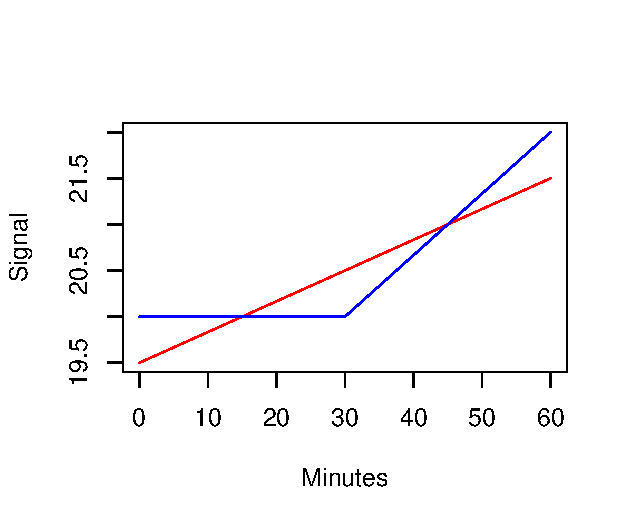
\includegraphics[scale=1.1,keepaspectratio=true]{./diagrams/TrendExample.pdf}
 % get.raw.data.1.pdf: 288x180 pixel, 72dpi, 10.16x6.35 cm, bb=0 0 288 180
 \end{center}
 \caption{Example of an artificial signal (in blue), simulating temperature, and (in red) its fitted linear trend}
 \label{fig:Trend Example}
\end{figure}

Residuals from trend in a case as depicted in figure \ref{fig:Trend Example} are large enough to elicit immediate suspect. But what happens on real-world signals, especially ``convective'', where variation may be more apparent than trend?

Checking some more quantitative aspect may prove helpful in these cases. For example we may try to compare relative non stationarity (of $w$ in our case) or non-steadinss (for $\overline{w'\theta'}$).

Figures \ref{fig:Rns detrend} and \ref{fig:Nst detrend} show what happens in CRA.01 case.

\begin{figure}[htp]
 \centering
 \begin{center}
 \includegraphics[scale=1.1,keepaspectratio=true]{./diagrams/WRnsDetrend.pdf}
 % get.raw.data.1.pdf: 288x180 pixel, 72dpi, 10.16x6.35 cm, bb=0 0 288 180
 \end{center}
 \caption{Relative non stationarity for wind component $w$ with (blue) and without (red) linear trend removal}
 \label{fig:Rns detrend}
\end{figure}

In figure \ref{fig:Rns detrend} we can see only one line of the expected two. This is because relative non-stationarity for wind component $w$ is very close to 0 and covered by the reference black line. But this adds very little to our knowledge: by the very way it's defined (linear regression of experimental data using time as independent variable) relative non-stationarity ``must'' drop to 0 (within roundoff errors).

More interesting is the behavior of non-steadiness, whose connection with linear trend removal is less strong. As figure \ref{fig:Nst detrend} suggests, some decrease occurs especially in correspondence of the two large peaks at 6 and 19. The smaller peak at 17 o'clock has remained perfectly unchanged however.

\begin{figure}[htp]
 \centering
 \begin{center}
 \includegraphics[scale=1.1,keepaspectratio=true]{./diagrams/WTNstDetrend.pdf}
 % get.raw.data.1.pdf: 288x180 pixel, 72dpi, 10.16x6.35 cm, bb=0 0 288 180
 \end{center}
 \caption{Non steadiness of $\overline{w'\theta'}$ with (blue) and without (red) linear trend removal}
 \label{fig:Nst detrend}
\end{figure}

The effect of detrending may then be beneficial in many cases, but we should take for granted specific situations will present where this strategy is not ideal. This is not surprising: nature is \emph{non}-linear, and imposing linearity on it is nothing more than a convenient artifice.

\subsubsection{Comparing the horizontal and vertical sigmas}

The standard deviations of horizontal and vertical wind can be used to feed atmospheric dispersion models, and the question arises of ``which'' standard deviations to use.

In modeling applications it is customary to use the vertical and cross-wind variances, and this suggests \emph{rotated} covariances are of interest. One practical question then is, whether non-rotated variances can be used instead. A positive answer makes sense, as computing non-rotated variances is of course simpler than with rotated variances.

On the other side, this positive answer is not physically impossible to achieve. In fact, the sum $\sigma_{u}^{2} + \sigma_{v}^{2} + \sigma_{w}^{2}$ (incidentally, twice the turbulent kinetic energy) is the \emph{trace} of the covariance matrix, and as such is invariant with respect to transformations like

\begin{equation}\label{eq:Matrix Conjugation}
    \mathbf{S} \mathbf{C} \mathbf{S}^{T}
\end{equation}

\noindent where $\mathbf{S}$ is non-singular. Rotation of reference, as performed in classical eddy covariance or planar fit, is a special case of this same transform, so we may expect the sum of the three wind component variances to stay unchanged under rotation. On reasonably not-too-complex terrain we may expect that the vertical component will not change too much, so the same must also be true for the sum of the two \emph{horizontal} variances.

That this desirable fact really happens is site-dependent, and connected to the average absolute magnitude of the second rotation angle. The verification is simple however.

In figure \ref{fig:Sigma_uv} we see the effect of reference rotation in CRA.01 set, by applying classical eddy covariance with 2 rotations.

\begin{figure}[htp]
 \centering
 \begin{center}
 \includegraphics[scale=1.1,keepaspectratio=true]{./diagrams/sigma_uv.pdf}
 % get.raw.data.1.pdf: 288x180 pixel, 72dpi, 10.16x6.35 cm, bb=0 0 288 180
 \end{center}
 \caption{Horizontal standard deviation $\sqrt{\sigma_{u}^{2} + \sigma_{v}^{2}}$ in non rotated vs rotated frame (data set: CRA.01)}
 \label{fig:Sigma_uv}
\end{figure}

As we can see, rotated and non rotated horizontal variances are practically the same in this case. By the rotation invariance of turbulent kinetic energy the same must be for vertical standard deviation. But skepticism is a virtue in science, so let's check directly in figure \ref{fig:Sigma_w}.

\begin{figure}[htp]
 \centering
 \begin{center}
 \includegraphics[scale=1.1,keepaspectratio=true]{./diagrams/sigma_w.pdf}
 % get.raw.data.1.pdf: 288x180 pixel, 72dpi, 10.16x6.35 cm, bb=0 0 288 180
 \end{center}
 \caption{Vertical standard deviation $\sigma_{w}^{2}$ in non rotated vs rotated frame (data set: CRA.01)}
 \label{fig:Sigma_w}
\end{figure}

The similarity of rotated and non-rotated variances is not the full story. Another interesting question is, whether some relation exists between horizontal and vertical component variance. In some dispersion models a linear relation between horizontal and vertical variances is assumed.

\begin{figure}[htp]
 \centering
 \begin{center}
 \includegraphics[scale=1.1,keepaspectratio=true]{./diagrams/sigma_uv_vs_w.pdf}
 % get.raw.data.1.pdf: 288x180 pixel, 72dpi, 10.16x6.35 cm, bb=0 0 288 180
 \end{center}
 \caption{Horizontal and vertical standard deviations compared (data set: CRA.01)}
 \label{fig:Sigma_uv_vs_w}
\end{figure}

The scattering we can see in figure \ref{fig:Sigma_uv_vs_w} is visually significant, yet the zero-passing linear model with its 0.1431 horizontal-to-vertical sigma suggests a much stronger horizontal standard deviation.

The existence of a clean relation between vertical and horizontal sigma allows site specific parameterizations of the sigma, which may be inserted in an existing atmospheric dispersion model, possibly after data have been classified in stable and convective; better even, measured standard deviations may be used directly in the model.

\subsection{A caveat: intrinsic limitations of eddy covariance}

Eddy covariance is a very powerful technique, and as such it is often used in many applications of immediate value, as for example quantifying fluxes of water or nutrients at the interface between an ecosystem and the Earth atmosphere.

In so doing many implicit assumptions may be taken for true, and a verification is often worth.

One assumption is terrain and canopy to be flat and uniform, and it often is self-evident whether this condition is met by a field experiment. Other assumptions may be much less intuitive, and related to the complex physics involved.

Experience shows eddy covariance exhibits a tendency to underestimate fluxes of carbon dioxide on night-time, under stable conditions (see e.g. \cite{Aubinet2012}). Some recent work (see in particular \cite{Aubinet2010}) highlight the possibility that divergence of horizontal flux contribute significantly. This is unfortunate, as the measurements needed are expensive and difficult (more towers, equipped with sonics and gas sensors, operating as in sync as possible). And ``unfortunately'' this effect may not explain all, or most, of the vertical exchanges of carbon dioxide, other factors (as flux from ground) having a very important impact on observed data.

Things may be even tougher than said. In cases where the ``forgotten terms'' are negligible other factors may also occur inducing eddy covariance to underestimate fluxes.

An interesting possible effect has been identified on rough terrain (see \cite{Sakai2001}), where low-frequency eddies may give an important contribution to fluxes. Long-frequency eddies might easily be washed out as ``trend'' by standard eddy covariance performed aggressively enough.

Possible solutions may come from including the non-intuitive aspects in models, and using them to validate measurements or devise new experimental methodologies. Two examples of this approach are shown in \cite{Canepa2010} and \cite{Montagnani2010}.

Anyway an appreciation of which is the (scientific and practical) context of measurements is fundamental to gain knowledge from measurements, and not just huge piles of data.

%*************************************************************************

\section{Ultrasonic anemometry for wind power plants}
\subsection{Introduction}

Wind power plant economic feasibility at a given site depends critically on whether enough wind is available, and if this wind can be used without harm (that is, at acceptable maintenance cost).

Traditionally the problem of \emph{plant siting} is addressed in stages, beginning with a CFD simulation performing the screening of comparativelky large regions (some kilometers) to locate the most promising sites for turbines. Once these prospective sites are defined, measurements are taken for limited periods (typically two months) to confirm the CFD predictions.

Measurements can be taken in many ways. Perhaps the most common (and supported by current technical standards) is by using mechanical anemometers installed at different heights above ground on a meteorological tower. Technical alternatives exist, and are gaining momentum: for example, using small SODAR system for remote sensing wind speed at many altitudes. And, of course, ultrasonic anemometers. This is the application we'll cover in this section.

Ultrasonic anemometers promise many improvements over mechanical anemometers. Two of these may be of special concerns to wind power plant designers: the ability of ultrasonic anemometers to see also the vertical wind (to which conventional anemometers are blind) and being able to measure turbulence directly. Both turbulence and vertical wind affect negatively the long term reliability of turbines. Said differently: they are connected to financial losses.

Just as a remind as we are dealing with money issues: large turbines cost a monstruous lot. I've heard orders of magnitude of 2 millions Euros per 1.6 MW (to date a medium size turbine, tending towards the small side). Such big investments are typically acted by banks, who are willing to give their money if and only if they foresee solid prospectives of yield.

This means banks wish to predict the future financial yield (or loss) associated to a prospective wind power plant the most accurately they can. As this is not always possible (banks often lack the accurate knowledge of wind) they tend to rely on the predictions made by designers, by ensuring these people follow sound modeling and measurement practice.

How do they do? The ``usual'' way in engineering: by verifying the plant designers and proposers have followed a rigid protocol. The protocol is quite detailed, and reflects the existing technical standards and the measurement technology available when they were first formulated. Currently, banks ask for ``certified'' measurements - and for measurements to be certified they must have been taken using ``certified instruments'' (to date, some mechanical anemometers). SODARs and ultrasonic anemometers are superior, and provide information banks would like very much to have, but are often not ``certified''. Or if they are, certificates are valid only in some countries and their automatic acceptance in other countries is not granted (neither impossible, however: as far as I know, for example, certificates emitted in Germany are accepted without discussion in Italy). To specify in precise legal terms what a ``certificate'' is lays much beyond the purpose of this manual, and we'll not pursue it any longer.

Rather, we focus on what ultrasonic anemometers may yield of interest to bankers, plant designers and other stakeholders, that conventional anemometers can't provide. Maybe will this contribute a little bit in improving the obsolete technical standards in current use?

\subsection{The function ''wind.power''}

Function \verb|wind.power| yields wind power and maintenance related data, both as sets of time-stamped vectors and overall indicators. Analyzed by skilled people, these numbers give detailed information about wind from a power production standpoint, to a level much refined than using mechanical instruments.

Before to proceed with the description, an important detail is worth mentioning: focus is on \emph{wind}, not turbines. Any specific turbine has its own power curve, which may be vastly different than power curves for other models. Electing one turbine as reference would be unfair to all others, so we'll not do. On the other side: is knowledge of wind is detailed enough, then computing a yield prediction is quite simple if the turbine power curve is known.

To invoke the function you may type this command:

\begin{verbatim}
wind.power(
  d,
  mode,
  cut.speed,
  lower.cut.speed,
  upper.cut.speed,
  verbose
)
\end{verbatim}

\noindent where

\begin{description}
 \item[d] is an object of class \verb|sonic.avg.data| containing the averaged data set from which to synthesize wind power related information.
 \item[mode] is an alphanumeric string containing the type of reference rotation to be made, with two possible values (``2.rotations'' and ``3.rotations'', with obvious meanings; default is ``2.rotations'').
 \item[cut.speed] is a boolean variable specifying whether processing should be limited to wind speed between specified limits (TRUE) or not (FALSE) (default: TRUE).
 \item[lower.cut.speed] is a wind speed signifying the lower limit to be considered if \verb|cut.speed| is TRUE ($\mbox{m/s}$; default: 6; ignored if \verb|cut.speed| is FALSE).
 \item[upper.cut.speed] is a wind speed meaning the upper limit to be considered if \verb|cut.speed| is TRUE ($\mbox{m/s}$; default: 6; ignored if \verb|cut.speed| is FALSE).
 \item[verbose] is a boolean flag specifying, if TRUE, that error and informational messages are to be printed, or not if FALSE (default: FALSE).
\end{description}

On successful completion function \verb|wind.power| returns an object of class \verb|sonic.wind.power.data|. In case of error a NULL value is returned, and if \verb|verbose| was seto to TRUE an error message is printed explaining what happened.

\subsection{Wind power specific quantities, and how they are computed in SonicLib}

Data requirements in wind power engineering do not coincide with eddy covariance and flux-related computations as we've seen in \ref{sec:Eddy Covariance}, although some overlap exists.

Two important problems in wind power engineering are how fast energy is produced, and whether wind conditions are likely to cause maintenance problems. The answer to both questions has a deep economical impact, determining in fact whether the plant will ever repay itself, and possibly produce some wealth.

Both questions are surprisingly tough, rooted in statistics as they are. Sensible answers based on sound rationality must start from measurements, and sonic anemometers give an important help as we'll see in the next sub-sections. It is worth mentioning that intuition is not as useful in this regard: we humans are prone to overestimate the impact of unusual conditions, which at many sites include a wind sufficiently strong to start turbine rotation.

\subsubsection{Mean and total power}

Maybe the most apparent indicator of wind quality at a site is its mechanical power. This is known to be proportional to the cube of wind speed,

\begin{equation}\label{eq:Wind power abstract form}
  P = k \cdot U^{3}
\end{equation}

The constant $k$ depends on turbine size, geometry and to some extent context, but in fact can be considered fixed provided a given turbine is selected. We may then concentrate on wind speed alone, introducing the corresponding wind factor,

\begin{equation}\label{eq:Wind power factor abstract form}
  F_{P} = U^{3}
\end{equation}

Expression (\ref{eq:Wind power factor abstract form}) is entirely abstract, as it involves wind speed as it is. We may rewrite it in more practical terms if we care to apply Reynolds decomposition to the total wind speed, $U = \overline{U} + U'$. By applying the binomial theorem we first get

\begin{equation}\label{eq:Wind power factor abstract form 2}
  U^{3} = \left( \overline{U} + U' \right)^{3} = \overline{U}^{3} + 3 \overline{U}^{2} U' + 3 \overline{U} U'^{2} + U'^{3}
\end{equation}

What we obtained is \emph{instantaneous} wind power, and we get very little from it. Average power is decidedly more interesting:

\begin{equation}\label{eq:Total wind power factor}
  \overline{U^{3}} = \overline{\overline{U}^{3} + 3 \overline{U}^{2} U' + 3 \overline{U} U'^{2} + U'^{3}}
\end{equation}

The right member in \ref{eq:Total wind power factor} may be rewritten taking into account $\overline{x+y} = \overline{x}+\overline{y}$ as

\begin{equation}\label{eq:Total wind power factor 2}
  \overline{U^{3}} = \overline{\overline{U}^{3}} + 3 \overline{\overline{U}^{2} U'} + 3 \overline{\overline{U} U'^{2}} + \overline{U'^{3}}
\end{equation}

In \ref{eq:Total wind power factor 2} we have $\overline{\overline{U}^{2} U'} = \overline{\overline{U}^2} \overline{U'} = \overline{\overline{U}^2} 0 = 0$, $\overline{\overline{U} U'^{2}} = \overline{\overline{U}} \overline{U'^{2}} = \overline{U} \overline{U'^{2}} = \overline{U} \sigma^{2}_{U}$ and $\overline{\overline{U}^{3}} = \overline{U}^{3}$ so that the formula can be rewritten as

\begin{equation}\label{eq:Total wind power factor 3}
  \overline{U^{3}} = \overline{U}^{3} + 3 \overline{U} \sigma^{2}_{U} + \overline{U'^{3}}
\end{equation}

The terms on right of \ref{eq:Total wind power factor 3} may be interpreted according to their physical meanings. $\overline{U}^{3}$ represents the average power, that is the part likely to be extracted from wind (at some given rendement) by a turbine.

The remaining part, $3 \overline{U} \sigma^{2}_{U} + \overline{U'^{3}}$, indicates the amount of power stored in turbulence. This power, not organized in some non-zero mean wind, is likely off the possibilities of use by wind turbines, at least directly, and the interesting question arises of large is it.

From a more practical side, computing the effective part of wind energy is straightformward: it is sufficient to get the period time average of wind speed, and raise to the cube. This is the meaning of \verb|mean.power.coef| and \verb|mean.power.coef.3|, the difference between the two coming from the first using only the horizontal components, and the second the whole vector.

Whether or not the turbulent quota of wind energy power affects turbines adversely might be an interesting research question, lying beyond this work' scope however, and we'll not follow it any seriously.


\subsubsection{Turbulence intensity}

An important indicator of wind quality (or better its lack) is \emph{turbulence intensity} defined as

\begin{equation}\label{eq:Turbulence intensity}
  T = \frac{\sigma_{U}}{\overline{U}}
\end{equation}

\noindent where $U$ represents instantaneous wind horizontal speed, and both mean and standard deviation have been computed on the same time interval.

Turbulence coefficient in SonicLib is computed in two ways. In the first, a turbulence intensity value is calculated for each time average (element \verb|T| in \verb|data|) using mean and variance of wind speed as computed when averaging the raw data set,

\begin{equation}\label{eq:Timewise turbulence coefficient}
  T\left( t \right) = \frac{\sigma_{U}\left( t \right) }{\overline{U}\left( t \right) }
\end{equation}

\noindent In the second, a global turbulence coefficient is introduced

\begin{equation}\label{eq:Overall turbulence coefficient}
  \overline{T} = \frac{\sum_{t \in \tau}\sigma_{U}\left( t \right) }{\sum_{t \in \tau}\overline{U}\left( t \right) }
\end{equation}

Of these, the first \ref{eq:Timewise turbulence coefficient} is the one to really consider. The second, \ref{eq:Overall turbulence coefficient}, stored in data element \verb|turb.coefficient|, is a sort of indication of the residual turbulence intensity due to the choice of averaging time. The possibility this indicator is nonzero (and possibly significantly large) depends on the fact that averaging time is standardized to 10 minutes, well below the mean position of the spectral gap, leading in many cases to an underestimation of time-wise wind speed standard deviation.

\subsubsection{Angle of wind to the horizontal plane}

Under ideal conditions the mean wind vector is characterized by a condition like $\overline{w} = 0$, that is, it belongs to the horizontal plane. 

Ideal conditions are very seldom found in nature, and it very often happen to the mean wind vector to form a non-zero angle to the horizontal. The value of this angle, a signed quantity, is computed as

\begin{equation}\label{eq:Angle to horizontal plane}
  \Phi\left( T \right) = \tan^{-1}\left( \frac{\overline{w}\left( T \right) }{\overleftarrow{U\left( T \right) }} \right) 
\end{equation}

\subsubsection{Friction velocity}

Friction velocity is an important indicator in wind power engineering, its value being often used to estimate wind profiles as

\begin{equation}\label{eq:Engineers wind profile}
  U\left( z \right) = \frac{u_{*}}{k} \log \frac{z}{z_{0}}
\end{equation}

Relation \ref{eq:Engineers wind profile} is strictly speaking valid only under neutral (adiabatic) conditions, that is when potential temperature stays constant with height above ground. Under stable and convective conditions an additional similarity term should be added to the logarithm, yielding a much more complex formula. On the other hand, existing wind turbines are able to produce energy in sensible amounts only at wind speeds in excess of, say, 6 to 8 $\mbox{m}/\mbox{s}$. By then, as shown in \cite{Oke1978}, the strong mixing caused by wind friction with ground surface is able to destroy any stable stratification or unstable convective structure, thus leveling anything towards the adiabatic.

So, we can assume \ref{eq:Engineers wind profile} makes some theoretical sense. SODAR profiles most often show a much more complex situation, sometimes with various layers of air overlapping with different properties. Even considering this, relation \ref{eq:Engineers wind profile} still tends to hold \emph{in the mean}, when many consecutive SODAR profiles are averaged together.

In lack of precise measurements of it, friction velocity is estimated by wind power engineers using the fixed value 0.1 $\mbox{m}/\mbox{s}$ (if one only measurement level is available), or by an expression like $U\left( z_{1} \right) - U\left( z_{2} \right) = \frac{u_{*}}{k} \log \frac{z_{1}}{z_{2}}$ when two measurement levels $z_{1}$ and $z_{2}$ exist. In both cases, the von Karman constant $k$ does not bother as its value is agreed to be practically equal to 0.4. The other quantity, the aerodynamic roughness length $z_{0}$, also does no harm as it is not considered with one measurement level, and it cancels out with two levels.

These simplified formulas often bear with them a large error whose extent is difficult to quantify merely relying on theory and a-priori information. Direct measurement by sonic anemometer sometimes shows quite different values, sometimes up to 0.3 $\mbox{m}/\mbox{s}$.

Because of this, friction velocity is computed by SonicLib, using the very same approach introduced in section \ref{sec:Eddy Covariance}:

\begin{equation}\label{eq:Friction Velocity for Wind Power}
  u_{*} = \left( \overline{u'w'}^{2} + \overline{v'w'}^{2} \right)^{1/4} 
\end{equation}

As with eddy covariance friction velocity is computed on every averaging step. Statistics, both overall and directional, may then be computed using standard R commands.

\subsubsection{Wind direction}

Wind provenance direction is an important tool: in conjunction with \verb|dir.mean| function it allows to detect spatial dis-uniformities which in case of wind power plants may be revealing.

Provenance direction is computed as

\begin{equation}\label{eq:Direction in wind power}
  D = \tan^{-1}\left( \frac{\overline{u}}{\overline{v}} \right) 
\end{equation}

\noindent using the actual R command like

\begin{verbatim}
  dir <- atan2(-u,-v) * 180/pi
\end{verbatim}

\noindent so that result is expressed according to the conventions of common use in the Earth sciences, North being designated as 0 and angles increasing clockwise. The \verb|atan2| function yields it results in the interval $-\pi \le \theta \le \pi$, so negative angles are produced. Converting them to positive form is easily accomplished by setting

\begin{verbatim}
  dir[dir < 0] <- dir[dir < 0] + 360.0
\end{verbatim}

\subsubsection{Rotation angles}

Rotation angles $\theta, \phi, \psi$ are used to compute the streamline reference system necessary for compiting other quantities - in particular the friction velocity.

Storing them allows to detect pointwise anomalies in data time series, for example by highlighting data records whose second rotation angle exceeds a given safety band.

\subsection{Preparing data for ``wind.power''}

We mentioned banks and bankers, and the standards they enforce as a condition to supply money. One standard does directly apply to our case: time averaging, which in wind power community is almost universally accepted to be 10 minutes.

This requirement closely connects to data being certifiable, an attribute allowing banks to reduce analysis costs, and very seldom might be changed: it's widely accepted by wind turbine community.

Preparing data for analysis by function \verb|wind.power| then demands data to be averaged using a call like this:

\begin{verbatim}
d <- average.sonic.file.set(
  dir.name,
  averaging.time=10
)
\end{verbatim}

\noindent where I've dropped all non-mandatory data.

\subsection{Examples}
\subsubsection{Economical feasibility}

Maybe the very first problem turbine designers (and banks) face is whether the plant to be will give some economical yield.

Indeed, investments for large plants are significant, in the order of 2 million Euro per 1.6 MW (to date a medium size machine: the really very large ones have reached rated power in the order of 6 MW, and dimensions tend to increase further). But as soon as the wind farm is connected to the electrical network any energy produced by it will generate financial yield.

For a plant to be economically feasible yield must exceed cost. Let's for the moment assume the plant owner is big enough to be able sustaining the whole installation and startup cost in a single large tranche, so that we may imagine the whole exit cash flow to occur just on the beginning of plant life. Of course this assumption is unrealistic, and here is where banks enter the overall picture, by providing loans so that the plant owner can pay bit by bit. But this is a detail which is not relevant to our example: all we have to know is that banks do not offer loans for free, so we should remember to increase the plant cost taking into account all financial loads.

As I mentioned, the plant produces some income. But this will occur slowly and, what matters maybe more, erratically: as much as wind power, more or less.

Here enters another factor: wind turbines do not endure forever, so it is common to consider a wind turbine lifetime of 20 years. After this time has elapsed the inevitable wear-out will have rendered maintenance cost prohibitive, not taking into account that by 20 years any current machine will be obsolete if technological development rate in wind turbines will remain as fast as it is now.

The morale is: a turbine must repay itself in \emph{less} than 20 years. All time in the 20 years past the repay period will generate a net income.

For the turbine to be let's say economically reasonable, the net income should be larger than the interest a bank would pay if you put all the money used to build, install and start the turbine to an account. Would this not be, then it would be more convenient to store the money in a bank and live more or less happily as financial speculators. But this means that the turbine must not only repay itself: it must generate real money.

Of course this analysis is strictly unilateral. There are other costs associated to wind power plants which to date do not enter the economic equation. To name one, the massive environmental impact of turbine themselves and the construction works associated to their deployment (and it is not excluded these costs sooner or later will be translated into some form of taxation). As we'll see in later examples there are still other costs, this time immediately relevant to turbines, which have not yet been considered.

But for now, let's assume our simplistic engineering-style analysis is exhaustive. Then we face a problem which looks hard enough: to predict in advance how much power will a given turbine generate if installed precisely at the desired site.

The fine details depend on the actual machine, so let's simplify in the extreme.

In general, a wind turbine will not extract a fixed fraction of the effective power stored in mean wind. At slow wind speed the turbine blades will stall and the rotor remains stuck. If wind increases above a limit depending on the specific turbine geometry and control policy the rotor will start its rotation, but will produce only a fraction of its nominal power. This ratio will progressively grow until wind reaches the minimum nominal production speed. If wind increases further the control policy of the wind turbine will intervene more and more energetically to allow the turbine to continue producing exactly the nominal power, while dissipating the excess (usually in mechanical form, fo example by reducing the blades' attack angle). Eventually, would wind exceed the safety speed of the turbine, the control system will reduce the blades attack angle to zero and act a powerful brake, thus stopping the machine to limit structural damages.

To place all these subjective considerations in perspective it may be worth specifying in some more detail what is meant as a slow of fast wind. Many large turbine start their rotation with mean wind in excess of 4 m/s. But the turbine will produce an infinitesimal amount of energy until, say, a 6 m/s, the nominal power being met at around 8 m/s. Turbine shutdown will occur would wind blow at more than 20 m/s. These figures are indeed \emph{large}. At current electricity remuneration, for a turbine to produce enough energy to repay it and generate some net income demands something around 70\% of time with wind speed between 6 and 20 m/s. This condition is quite infrequent in the areas where most of our data sets have been collected, but do indeed occur in many places of the World. Offshore and mountain crest sites are not rare.

What of small turbines instead? To date machines rated at 1 kW or even less are not uncommon, and in many European sites is indeed likely to see one or two in town blocks, installed over roofs. These small-sied machines are lightweight constructed and because of this operate at a somewhat smaller wind speed. Rotation very often begins at 2 m/s, and full productivity is attained between 6 and 8 m/s. Of course the tiny nacelles of these amateur power producer plants are too small to host an emergency brake, and no blade rotation is possible. Then, would wind blow at an excessive speed these small-sized turbines are likely to disintegrate. The logics behind all that is fairly simple: the owner wait until tempest has gone and buys just another.

As I mentioned, in order to avoid excessive complications we'll stay simple. In practice, we imagine the turbine to operate ideally (that is, at full nominal power) within a fixed speed range, say 6 to 20 m/s. Stated this way, our problem reduces to determining how much time does wind speed stays within these limits.

We need to draw this information from wind measurements taken for a limited time at the prospective installation site. Wind is infamous for its erratic behavior however, and so we can see a trouble: the measurement period might be too short, or chosen so to not represent the climatological site reality.

But, let's begin with the how. The method commonly used to solve the problem assumes wind speed can be modeled as a random variable following a Weibull distribution. The trick then is to fit an instance of the Weibull distribution from data, write it as probability density function $p(x;\alpha,\beta)$, then derive the probability that wind speed is between the desired limit as

\begin{equation}\label{eq:Wind probability of being between specified limits}
  \mathbf{P}\left\lbrace U_{min} \le U \le U_{max} \right\rbrace = F(U_{max};\alpha,\beta) - F(U_{min};\alpha,\beta)
\end{equation}

\noindent where $F(U_{max};\alpha,\beta) - F(U_{min};\alpha,\beta) = \int_{U_{min}}^{U_{max}} p(x;\alpha,\beta) dx$ is the difference between the cumulative distribution functions computed at interval endpoints.

The problem with Weibull distribution is its parameters $\alpha$ and $\beta$ are not simple to estimate. The Weibull density is

\begin{equation}\label{eq:Weibull Density}
	p(x;\alpha,\beta) = \left\lbrace
		\begin{array}{cr}
			\frac{\alpha}{\beta}
			\exp -(\frac{x}{\beta})^{\alpha}
			(\frac{x}{\beta})^{(\alpha - 1)} & x > 0 \\
			0 & x \le 0 
		\end{array}
	\right. 
\end{equation}

\noindent and its first two moments are

\begin{equation}\label{eq:Weibull Mean}
  \mu = \beta \Gamma \left( 1 + \frac{1}{\alpha} \right)
\end{equation}

\noindent and

\begin{equation}\label{eq:Weibull Standard Deviation}
  \sigma = \beta \sqrt{\Gamma \left( 1 + \frac{2}{\alpha} \right) - \Gamma \left( 1 + \frac{1}{\alpha} \right)^{2}}
\end{equation}

Taken together, equations \ref{eq:Weibull Mean} and \ref{eq:Weibull Standard Deviation} constitute a system in the two unknowns $ \alpha $, $ \beta $. This non-linear system is obviously closed, but a solution is not easy to find in explicit terms. To solve it we need then to use a numerical method, and we ought to build it in R.

Before to start solving the non-linear system as it is, we may do some manipulations in order to make the problem simpler. Indeed, if we divide \ref{eq:Weibull Standard Deviation} by \ref{eq:Weibull Mean} we get an expression whose value depends on $ \alpha $ only:

\begin{equation}\label{eq:Weibull ratio estimation}
  \frac{\sigma}{\mu} = \sqrt{\frac{\Gamma \left( 1 + \frac{2}{\alpha} \right)}{\Gamma \left( 1 + \frac{1}{\alpha} \right)^{2}} - 1}
\end{equation}

This expression may be seen as an equation allowing to identify the value of $ \alpha $, given $ \frac{\sigma}{\mu} $. But unfortunately an analytic solution can not be found - at least simply. A numerical solution may be found easily however, the function

\begin{equation}\label{eq:Weibull ratio estimation as function}
  f\left( \alpha \right) = \sqrt{\frac{\Gamma \left( 1 + \frac{2}{\alpha} \right)}{\Gamma \left( 1 + \frac{1}{\alpha} \right)^{2}} - 1}
\end{equation}

\noindent appearing to the right of \ref{eq:Weibull ratio estimation} is continuous in the interval $ (0,\infty] $ with $ \lim_{x \rightarrow 0^{+}} f(x) = +\infty $ and $ \lim_{x \rightarrow \infty} f(x) = 0 $.

For any (necessarily positive) value of the ratio $ \frac{\sigma}{\mu} $ equation \ref{eq:Weibull ratio estimation} has exactly one solution. Once this solution $ \alpha^{*} $ has been found, estimating the parameter $ \beta $ is straightforward:

\begin{equation}\label{eq:Weibull beta estimation}
  \beta^{*} = \frac{\mu}{\Gamma \left( 1 + \frac{1}{\alpha^{*}} \right)}
\end{equation}

If we use the whole data set CRA.01 using a call like

\begin{verbatim}
w <- wind.power(d, cut.speed=FALSE)
\end{verbatim}

\noindent we get Weibull values $ \alpha = 1.59 $ and $ \beta = 3.04 $. The general shape of the Weibull density corresponding to these two parameters is shown in figure \ref{fig:CRA01 Weibull} for reference.

\begin{figure}[htp]
 \centering
 \begin{center}
 \includegraphics[scale=0.80,keepaspectratio=true]{./diagrams/CRA01_Weibull.pdf}
 % get.raw.data.1.pdf: 288x180 pixel, 72dpi, 10.16x6.35 cm, bb=0 0 288 180
 \end{center}
 \caption{Density of estimated Weibull wind speed distribution (data set: CRA.01)}
 \label{fig:CRA01 Weibull}
\end{figure}

Weibull probability density says quite a little visually but an important thing: wind speed extends to quite large maximum values. Indeed we'd like a more intuitive economical indicator, and this is the cumulative probability distribution, or better even its one complement, showing the probability a given wind speed is exceeded. The value of this probability gives a rough indication of how often will the turbine produce valuable energy.

\begin{figure}[htp]
 \centering
 \begin{center}
 \includegraphics[scale=0.80,keepaspectratio=true]{./diagrams/Weibull_Exceedance_Probability.pdf}
 % get.raw.data.1.pdf: 288x180 pixel, 72dpi, 10.16x6.35 cm, bb=0 0 288 180
 \end{center}
 \caption{One-complement of the CDF corresponding to estimated Weibull wind speed distribution (data set: CRA.01)}
 \label{fig:CRA01 Weibull Exceedance}
\end{figure}

Figure \ref{fig:CRA01 Weibull Exceedance}  just shows this indicator. Here the likelihood of production is clearly visible. Would for example the turbine start producing at 4 m/s, we could expect something in the order of 20 \% of productive time (and an 80 \% of idle time: not a very good thing, in financial terms). The precise value is 21.3 \%.

When dealing with economical problem, the bare estimation of how many hours will be productive is a good starting point (especially to prove a site is \emph{not} suitable for a wind power plant) but is usually not sufficient. A more interesting subject is having an indication of how much power will be actually produced and, optimistically assuming a one-to-one sell ratio, how much money will be earned at a specified tariff level.

Answering this advanced question demands however much more information, namely the turbine response curve. Response curves are typically given in form of tables, with power produced at some given speeds. Some of these tables also contain air density as a second input, lighter air containing less momentum at the same wind speed. An example of table is given for an existing small (10 kW) turbine:

\begin{tabular}{cc}
\hline 
\rule[-2ex]{0pt}{5.5ex} Wind speed (m/s) & Power (kW) \\ 
\hline 
\rule[-2ex]{0pt}{5.5ex} 1 & 0 \\ 
\rule[-2ex]{0pt}{5.5ex} 2 & 0 \\ 
\rule[-2ex]{0pt}{5.5ex} 2.5 & 0.4 \\ 
\rule[-2ex]{0pt}{5.5ex} 4 & 0.9 \\ 
\rule[-2ex]{0pt}{5.5ex} 5 & 2.3 \\ 
\rule[-2ex]{0pt}{5.5ex} 6 & 3.3 \\ 
\rule[-2ex]{0pt}{5.5ex} 7 & 4.9 \\ 
\rule[-2ex]{0pt}{5.5ex} 8 & 6.7 \\ 
\rule[-2ex]{0pt}{5.5ex} 9 & 8.1 \\ 
\rule[-2ex]{0pt}{5.5ex} 10 & 9.3 \\ 
\rule[-2ex]{0pt}{5.5ex} 11 & 9.8 \\ 
\rule[-2ex]{0pt}{5.5ex} 11.5-25 & 9.8 \\ 
\hline 
\rule[-2ex]{0pt}{5.5ex}  &  \\ 
\end{tabular} 

We conclude this section with a caveat. Not all wind turbine plants are justified in economical terms. That is, there may be circumstances where the analysis just depicted makes no sense. An example may be the case of a wind turbine used to lift water on a small island where no power supply is available. In such a case the good is not some energy which can be sold, but rather the benefit of having water lifted, and then available to human use. If so, any output from the wind turbine is valuable whatever its actual amount: in the best scenario the water lifted by wind is sufficient to fulfill local demand. In the worst, it's anyway some spare of precious combustible. In these cases other kind of analyses should be made - which we'll not deepen here for reasons of space.


\subsubsection{Is wind speed really Weibull-distributed?}

In technical literature on wind power plant it is often assumed that wind follows a Weibull distribution, and in the preceding section we have used this hypothesis as well and drawn plant feasibility conclusion based on it.

But: it is always true for wind to be Weibull? Stated this (strong) way, the question is unlikely to have a positive answer. And in fact we may exhibit a counterexample, just based on the same CRA.01 data set we've just used in the preceding section.

By inspecting the output structure of \verb|wind.power| we discover in fact two other fields related to Weibull distribution, namely \verb|weibull.statistic| and \verb|weibull.probability|. As explained in section \ref{sec:sonic.wind.power.data}, these fields report the result od Kolmogorov-Smirnov test made comparing the empirical cumulative distribution function to the modeled Weibull. Of these values \verb|weibull.probability| is of more immediate interest to our case: it specifies the probability that our data set sample has been drawn from a Weibull distribution of specified parameters.

The value found on CRA.01 set, 0.453, is quite small: less than a 50 \% chance! So, we can't honestly claim wind to be Weibull-distributed. We may even see it, if we plot the modeled Weibull density along with the gamma estimate of experimental data's, as we do in figure \ref{fig:CRA01 Weibull and Experimental}.

\begin{figure}[htp]
 \centering
 \begin{center}
 \includegraphics[scale=0.80,keepaspectratio=true]{./diagrams/CRA01_Weibull_exper.pdf}
 % get.raw.data.1.pdf: 288x180 pixel, 72dpi, 10.16x6.35 cm, bb=0 0 288 180
 \end{center}
 \caption{Density of estimated Weibull wind speed distribution overlapped to gamma estimate of empirical density (in red; data set: CRA.01; no cut speeds)}
 \label{fig:CRA01 Weibull and Experimental}
\end{figure}

However: the empirical speed density is not that \emph{dramatically} far from a Weibull, at least from a visual standpoint. If we limit attention to wind speeds whose value lays within the turbine operational interval 4 to 25 m/s as we've seen in the preceding section, Weibull probability rises to 0.814. The corresponding plot is shown in figure \ref{fig:CRA01 Weibull and Experimental Cutted}.

\begin{figure}[htp]
 \centering
 \begin{center}
 \includegraphics[scale=0.80,keepaspectratio=true]{./diagrams/CRA01_Weibull_exper_cut.pdf}
 % get.raw.data.1.pdf: 288x180 pixel, 72dpi, 10.16x6.35 cm, bb=0 0 288 180
 \end{center}
 \caption{Density of estimated Weibull wind speed distribution overlapped to gamma estimate of empirical density (in red; data set: CRA.01, with lower and upper cut speeds respectively equal to 4 and 25 m/s)}
 \label{fig:CRA01 Weibull and Experimental Cutted}
\end{figure}

We retained less data (37 instead of 144), and the peaky result is more similar visually to a Weibull density. What all that means? An interpretation is, the Weibull model is not too bad, even is measurements are taken very precisely with an ultrasonic anemometer.


\subsubsection{Why Weibull?}

The Weibull density is characterized by an asymmetric shape (which fits well with wind speed non-negativity), and a tail which may be fat or lean depending on the value of $ \alpha $.

Of course this is not the only distribution gifted of the same properties. Among the ones sharing the same attributes, at least in given ranges of $ \alpha $ and $ \beta $, we can find the log-normal, the Gamma, the Chi-square, and others. Why not using them?

Indeed, some distribution other than Weibull might be computationally simpler. For example, to fit a log-normal distribution one should first identify its two parameters, (the so-called log-normal mean $m$ and standard deviation $s$) starting from data mean $\mu$ and standard deviation $\sigma$. This operation may be carried on entirely on symbol manipulation, instead of using numerical methods as we have been compelled to in case of the Weibull distribution, as we can see from the two relations

\begin{equation}\label{eq:Lognormal mean}
	m = \log \mu - \frac{1}{2}\log \left[1 + \left(\frac{\mu}{\sigma}\right)^{2} \right]
\end{equation}

\noindent and

\begin{equation}\label{eq:Lognormal standard deviation}
	s = \sqrt{\log \left[1 + \left(\frac{\mu}{\sigma}\right)^{2} \right]}
\end{equation}


%*************************************************************************

\chapter{Visualizing Data and Their Structure}
\section{Plotting data the simple way}

One important visualization of data, and maybe one of the most common, is just plotting them as functions of time.

SonicLib does not provide a function to perform this task, the almost-almighty \verb|plot| command of base R being orders of magnitude more than plain sufficiency. Here we give some idea, however, by showing some practical interactive examples.

If you are not familiar with R reading this section may prove worth the bit effort, both for its own utility and the possibility to extend knowledge gained here to customize the SonicLib diagrams presented in later sections.

As mentioned shortly, the plotting command used in R is

\begin{verbatim}
plot(x, y, ...)
\end{verbatim}

\noindent where \verb|x| and \verb|y| designate the two vectors (of the same length) containing the $x$ and $y$ coordinates on the plotting plane. Ellipsis are a placeholder indicating the (possibly long) set of parameters.

Parameters are of course of paramount importance, as their sensitive use allows to produce publication-quality plots with little effort. They exist in an impressive number, and if you like to browse among them we kindly invite you to have a look at R help (just as a starter, you may begin by giving command \verb|?plot| from within an R session; as your needs become more advanced you may want to consult specialized texts like \cite{Murrell2006}).

%*************************************************************************
\subsection{Example: Understanding non-stationarity with time domain plots}

As a first practical example suppose we investigate the reason of why relative non-stationarity of $w$ peaked at 15:30 in CRA.01 data set, but not at 15:00. As we've discovered in section \ref{sec:Sane skepticism} data set CRA.01 is characterized by a ``normal'' value of relative non stationarity on $w$, from which a few distinct peaks emerge. The one occurring at 15:30 characterizes for its narrow span, suggesting an unusual event suddenly coming in.

SonicLib raw data are stored in hourly file, whose naming convention (explained in \ref{sec:FileFormat}) allows to predict the one we're interested in is \verb|20100516.15.csv|: our first task is grabbing it into the R session:

\begin{verbatim}
f <- get.raw.data("../TestData/CRA.01/20100516.15.csv", verbose=TRUE)
\end{verbatim}

Having specified \verb|verbose=TRUE| allows to check for any error message. The function completed printing no message to session, so we can deduce all went right as far as SonicLib is concerned. But the final proof is in the result itself, which we may check giving the command

\begin{verbatim}
str(f)
\end{verbatim}

This done, the system answers presenting a short sample of the data stored into file:

\begin{verbatim}
List of 2
 $ data         :'data.frame':	35990 obs. of 7 variables:
  ..$ time.stamp: num [1:35990] 0 0 0 0 ...
  ..$ u         : num [1:35990] -0.27 -0.61 ...
  ..$ v         : num [1:35990] -2.18 -1.89 ...
  ..$ w         : num [1:35990] 0.28 0.06 ...
  ..$ t         : num [1:35990] 15.4 15.3 ...
  ..$ q         : num [1:35990] 273 277 ...
  ..$ c         : num [1:35990] 16.2 16.2 ...
 $ sampling.rate: num 10
 - attr(*, "class")= chr "sonic.raw.data"
>
\end{verbatim}

The summary given by \verb|str()| is interesting and infrmative: it allows to get an impression of the nature of data, and a bit of intuition will easily arrive to figure out the structure. R allows other summaries however: for example, \verb|summary()| applied to a data frame returns a complete statistic report of each column.

Among all other useful things, command \verb|str()| allows us to understand where the data we're interested in may be found. We may decide to store this knowledge in our neurons for later use, or make use of some other commands to make our life less painful now. We follow this second path, by isolating time stamp and vertical wind component in variables whose names is easy to remind and shorter to type:

\begin{verbatim}
t.s <- f$data$time.stamp
w <- f$data$w
\end{verbatim}

We may now engage the real problem, visualizing data. We may begin with the simplest possible plot:

\begin{verbatim}
plot(t.s,w)
\end{verbatim}

Result is shown in figure \ref{fig:Simple plot 0}. As you can see, the result is absolutely unsatisfactory! In fact, if no specific option is given the R default version of \verb|plot| just builds a scatter plot, with open circles at every data point. The circles are wide, and data plots in large number: the final result is filling a third of the plot with a black band, losing completely any hope to follow the actual variation.

\begin{figure}[htp]
 \centering
 \begin{center}
 \includegraphics[scale=1.1,keepaspectratio=true]{./diagrams/SimplePlot0.pdf}
 % get.raw.data.1.pdf: 288x180 pixel, 72dpi, 10.16x6.35 cm, bb=0 0 288 180
 \end{center}
 \caption{Variation of vertical wind speed with time, from 15:00 to 16:00 in CRA.01 set}
 \label{fig:Simple plot 0}
\end{figure}

What we really desire in fact is a \emph{line plot}. In R this means to specify an additional parameter:

\begin{verbatim}
plot(t.s, w, type="l")
\end{verbatim}

The new result is shown in figure \ref{fig:Simple plot 1}.

\begin{figure}[htp]
 \centering
 \begin{center}
 \includegraphics[scale=1.1,keepaspectratio=true]{./diagrams/SimplePlot1.pdf}
 % get.raw.data.1.pdf: 288x180 pixel, 72dpi, 10.16x6.35 cm, bb=0 0 288 180
 \end{center}
 \caption{Variation of vertical wind speed with time, from 15:00 to 16:00 in CRA.01 set}
 \label{fig:Simple plot 1}
\end{figure}

The result of our second attempt is a bit better than before: we now have a better impression of actual data variation. Yet the plot is still unsatisfactory: to begin with, axes descriptions are at best uninformative to people not already knowing the facts.

A better approach would be to indicate clearly what the variables are, and which measurement units have been used. This is simple for the vertical axis. But what of the horizontal? In this case the figure caption says the plot refers to an entire hour, and the range suggests seconds are used (this is consistent with the time stamp definition within SonicLib raw data files once read in memory). Seconds demands a lot of space to be printed: minutes may be preferable? And what of axis name? To tell, or to remove?

We try by improving the vertical axis, and removing axis name from the horizontal. We also convert to minutes:

\begin{verbatim}
plot(t.s/60, w, type="l", ylab="w (m/s)", xlab="")
\end{verbatim}

Here the result:

\begin{figure}[htp]
 \centering
 \begin{center}
 \includegraphics[scale=1.1,keepaspectratio=true]{./diagrams/SimplePlot2.pdf}
 % get.raw.data.1.pdf: 288x180 pixel, 72dpi, 10.16x6.35 cm, bb=0 0 288 180
 \end{center}
 \caption{Variation of vertical wind speed with time, from 15:00 to 16:00 in CRA.01 set}
 \label{fig:Simple plot 2}
\end{figure}

Figure \ref{fig:Simple plot 2}, too, is far from ideal, yet much better than \ref{fig:Simple plot 0}. We might now try to place ticks not where R likes, but where our aesthetical sense could suggest. Or, me may adopt a lighter color for $w$.

All these improvements can be made adding parameters. We might go on, refining our plot further, but we imagine you got the message. Any details may be found in \cite{RManual}.

But, we notice an important thing. Our last graph is finally \emph{useful}: it shows us a large change occurred in wind \emph{variation} (a second order like statistics). This variation occurs exactly where we expected it, in the second half-hour. Last but not least, if placed in a presentation would make immediately the point even to a casual listener.

Before closing this example we love to highlight an important concept:

Plotting data involves of course learning R powerful graphics commands, but its real purpose is \emph{telling a story}, and making a point. No story, poor graph. Before delving into the development of the fanciest plot it is advisable to think first what we would like to transmit.

This in turn demands a clear understanding of whom our story is aimed at. Stated differently, writing programs or using a top-notch software package is at least 90\% human relation and communication, and 10\% technology (and not be impressed by the commonly observed fact that industry rewards technology 90\% and good communication 10\%: it says a lot about the past, present and, likely, future ``financial crises'': Buggy by Design?)

Sure this manual has not space enough to get deep on this essential point, but fortunately there are many excellent references. Among them the authors have used (and found subjectively useful) \cite{Maindonald2007} and \cite{Venables2002}.

We proceed now to check where the anomalous relative non-stationarity comes from. According to its definition, the relative non-stationarity is proportional to the difference between minimum and maximum value of signal regression line. As the regression line is so important, it would be nice showing it.

The first step to get distinct regression lines is partitioning data with respect to time in first and second half hour. We may accomplish this result, by using the powerful indexing capabilities of R on the time stamp:

\begin{verbatim}
t.lower <- t.s <= 1800
t.upper <- t.s >  1800
\end{verbatim}

\verb|t.lower| and \verb|t.upper|, generated this way, are two boolean vectors of same length as \verb|w|. These vectors can be used to select the upper and lower part of vertical wind speed:

\begin{verbatim}
w.lower <- w[t.lower]
w.upper <- w[t.upper]
\end{verbatim}

We used time stamps as a selection tool, but it is not wise to employ them as independent variable in linear modeling. This, because in SonicLib raw data files time stamps are allowed to be integer (they are, in CRA.01 set) so repeated stamps are possible. An alternative is using positional indices, and we'll do this method. Partitioning indices is the same as with $w$; in addition we scale them so they can function as replacement of minutes.

\begin{verbatim}
idx <- 1:length(w)
idx.lower <- idx[t.lower]/600
idx.upper <- idx[t.upper]/600
\end{verbatim}

The next step is computing the models themselves. This is done using command \verb|lm()|, using partitioned indexes as independent variables, and partitioned $w$ as dependent:

\begin{verbatim}
l.lower <- lm(w.lower~idx.lower)
l.upper <- lm(w.upper~idx.upper)
\end{verbatim}

The result we obtained can then be inspected by giving commands \verb|l.lower| and \verb|l.upper| respectively. This is what we get with the lower half hour:

\begin{verbatim}
Call:
lm(formula = w.lower ~ idx.lower)

Coefficients:
(Intercept)    idx.lower  
 -0.0422577    0.0004308
\end{verbatim}

\noindent And this is the upper:

\begin{verbatim}
Call:
lm(formula = w.upper ~ idx.upper)

Coefficients:
(Intercept)    idx.upper  
   0.059042    -0.001693
\end{verbatim}

Note slope and intercept have opposite signs in the two cases. But values are small enough to make very difficult to predict visually what happens. We wish to display data and the regression lines, and our first attempt is by applying the command \verb|abline()|, applied to the regression models after having plotted the actual data:

\begin{verbatim}
plot(idx/600, w, type="l", ylab="w (m/s)", xlab="")
abline(l.lower, col="red")
abline(l.upper, col="blue")
\end{verbatim}

\noindent The result is shown in figure \ref{fig:Simple plot 3}.

\begin{figure}[htp]
 \centering
 \begin{center}
 \includegraphics[scale=1.1,keepaspectratio=true]{./diagrams/SimplePlot3.pdf}
 % get.raw.data.1.pdf: 288x180 pixel, 72dpi, 10.16x6.35 cm, bb=0 0 288 180
 \end{center}
 \caption{Variation of vertical wind speed with time, from 15:00 to 16:00 in CRA.01 set. In red the regression line computed on first half hour; in blue the regression line of second half hour.}
 \label{fig:Simple plot 3}
\end{figure}

This is not the best we may do: according to the way \verb|abline()| operates on regression lines, the whole span of independent variable is used, and this gives a really misleading view: it would be much better to plot the two lines only where they are defined. To do this, we could evaluate the regression models in correspondence of their definition intervals, then plot them.

The first step, evaluating the models in correspondence of the independent variable values, may be done the straightforward way once we know the regression coefficients:

\begin{verbatim}
m.lower <- l.lower$coefficients
m.upper <- l.lower$coefficients
\end{verbatim}

Proceeding this way instead of copying their values shown previously we get coefficients in full precision. Because R is done, \verb|m.lower[1]| represents the intercept and \verb|m.lower[2]| the slope of regression model \verb|l.lower| (and identically with \verb|l.upper|).This allows to perform our estimation:

\begin{verbatim}
w.est.lower <- m.lower[1] + idx.lower*m.lower[2]
w.est.upper <- m.upper[1] + idx.upper*m.upper[2]
\end{verbatim}

\noindent We are now ready to plot:

\begin{verbatim}
plot(idx/600, w, type="l", ylab="w (m/s)", xlab="")
lines(idx.lower,w.est.lower,col="red",lwd=3)
lines(idx.upper,w.est.upper,col="blue",lwd=3)
\end{verbatim}

The command \verb|lines()| plots a line graph without removing the underlying graphics, as \verb|plot()| would do by default. Parameter \verb|lwd| specifies the line width, with a minimum value of 1; value 3 is a sensible choice to make the line visible. The result is \ref{fig:Simple plot 4}.

\begin{figure}[htp]
 \centering
 \begin{center}
 \includegraphics[scale=1.1,keepaspectratio=true]{./diagrams/SimplePlot4.pdf}
 % get.raw.data.1.pdf: 288x180 pixel, 72dpi, 10.16x6.35 cm, bb=0 0 288 180
 \end{center}
 \caption{Variation of vertical wind speed with time, from 15:00 to 16:00 in CRA.01 set. In red the regression line computed on first half hour; in blue the regression line of second half hour.}
 \label{fig:Simple plot 4}
\end{figure}

The two regression lines are different, as we had seed when printing the model numerical values. But visually, their dissimilarity seems not striking.

%*************************************************************************
\subsection{Visualizing directional dependencies using R as it is}

One common reason of non-uniformity is connected to the different ``history'' experienced by wind as it flows through different environments. An indicator of this history is wind provenance direction.

One way to display the dependence of a variable on wind direction is a scatter plot with the wind direction used as an independent variable. But such a diagram is quite uninformative if we employ a scatter plot of the usual kind, like the one shown in figure \ref{fig:Normal directional scatter plot}, showing the change of the ratio of friction velocity to the wind speed with respect of a ``long'' data set.

\begin{figure}[htp]
 \centering
 \begin{center}
 \includegraphics[scale=1,keepaspectratio=true]{./diagrams/UstarOverVel_vs_Dir_Standard.pdf}
 % get.raw.data.1.pdf: 288x180 pixel, 72dpi, 10.16x6.35 cm, bb=0 0 288 180
 \end{center}
 \caption{Directional scatter plot of $u_{*}/U$ drawn using the standard ``plot'' command}
 \label{fig:Normal directional scatter plot}
\end{figure}

The reason figure \ref{fig:Normal directional scatter plot} is not the best is the heavy clutter of circles: if data are too much a significant danger exists they overlap in a way not allowing to appreciate where they're most concentrated.

An alternative in this case is using command \verb|smoothScatter|, now part of the standard R distribution. The syntax is identical to \verb|plot|'s, but instead of small circles in correspondence of data points, pixel in shades of gray are drawn proportional to the number of data points in the nearby. In practice, the higher the concentration, the darker the tone. As we may see in figure \ref{fig:Improved directional scatter plot}.

\begin{figure}[htp]
 \centering
 \begin{center}
 \includegraphics[scale=1,keepaspectratio=true]{./diagrams/UstarOverVel_vs_Dir.pdf}
 % get.raw.data.1.pdf: 288x180 pixel, 72dpi, 10.16x6.35 cm, bb=0 0 288 180
 \end{center}
 \caption{Directional scatter plot of $u_{*}/U$ drawn using command ``smoothScatter''}
 \label{fig:Improved directional scatter plot}
\end{figure}

What happens around 130 degrees? As we may see, the ratio of friction velocity to wind speed is close to a fashionable 10\% in all directions, with the exception of the sector 100 to 170 degrees, where we can see a sharp rise to a 30\%, followed by a complementary sharp decrease.

Visual inspection of aerial photographs of field site suggests a possible reason: a tall and wide tree standing to the SE of measurement point, at around 25 meters distance. In theory, fixed stations should be placed at least at a distance ten times the height of major obstructions at any possible direction. But this requirement is really difficult to fulfil in practice, especially in densely populated areas. And more so at \emph{urban} sites. 

If this is the case, a directional diagram of some key turbulence indicators may work well as a data quality assessment tool. It may also be helpful in quality \emph{assurance}, for example by labeling data associated to wind direction from some critical directions. If ``all'' directions are critical, then a convincing argument for relocating an existing station is also easy to build.

\section{SonicLib-specific Plots and Related Functions}

\subsection{Function dir.mean}
\subsubsection{Function use}

To use \verb|dir.mean| the following command should be issued:

\begin{verbatim}
dir.mean(
  dir,
  val,
  width,
  step,
  confidence,
  boot.size,
  conf.level
)
\end{verbatim} 

\noindent where

\begin{description}
 \item[dir] Vector containing direction values for each data set elements (degrees from North; no default).
 \item[val] Vector, having the same dize as ``dir'', and containing all values for each data set element (unit depends on actual value meanings; no default).
 \item[width] Sector width (degrees; default = 11.25).
 \item[step] Angle between the center directions of two consecutive steps (degrees; default = 1).
 \item[confidence] Method to be used when computing confidence intervals (alphanumeric string, with possible values ``none'' and ``boot''; default: ``boot'').
 \item[boot.size] Sample size to be used when computing confidence limits using bootstrap method (positive integer number; default = 1000; this value is ignored if ``confidence'' is not ``boot'').
 \item[conf.level] Value of the confidence level at which confidence intervals are computed (default = 0.95).
\end{description}

The result is an instance of an object \verb|dir.stat| in case of successful completion, or NULL otherwise.

\subsubsection{Separate or overlapping sectors?}

If the function defaults are used, sectors are guaranteed to overlap widely as each of them is 11.25 degrees wide (half  the familiar 16-wind-sectors rule), and the sector-to-sector angular spacing is just 1 degree.

This way, passing from a sector to the next many data values get the chance of being counted twice. Is this a big deal? In many cases ``no'' could be an appropriate answer: an indicative mean is just good.

This needs not be the universal case however. Proper selection of \verb|width| and \verb|step| allows customization. A common non-default choice consists in selecting 16 sectors, with \verb|width=22.5| and \verb|step=22.5|, in which case sectors overlap only on their boundary (a line, with zero area), behaving as practically separate.

\subsubsection{Confidence intervals}

Function \verb|dir.mean| provides parameters allowing to estimate confidence intervals on each directional mean. The meaning of confidence interval is not to give an idea of dispersion of values around the mean (although it could be mathematically related to it), but rather to specify an interval such that the true directional mean belongs to it at a specified confidence level.

The true and computed directional means should in fact not be confused, the latter being an estimate of the former, whose actual value is not a priori known.

Confidence limits can be used as a visual tool (they will, using directional mean plotting functions within SonicLib), but may also be used numerically to solve common problems on statistically firmer ground than just proceding intuitively. Suppose for example you are interested in checking the value of friction velocity seen by wind coming from a given direction in, say, winter and summer - possibly to check for changes in turbulence generation by deciduous shrubs upstream.

Without confidence limits you'd presumably get the directional means computed in the two periods, compare them, and likely decide they are somewhat different. This is not a strong conclusion, indeed: the two numerical values of means along the same direction may not be equal, but this do not prove beyond any doubt their true values to be also different.

If we have confidence interval at hand, solving the problem in more meaningful terms is easier: it suffices to see whether the two confidence intervals have void intersection or not. In the first case you can be ``reasonably sure'' (within confidence level) the true directional means are different. In the second, you can't exclude their equality. Even if the overlap zone is small compared to interval overall size.

Similar considerations can be made for other problems of practical interest. For example: is temperature changing with wind direction, or not? Overall, confidence limits are a precious indication.

\subsubsection{Examples}

Using function \verb|dir.mean| is straightforward: all you need are two equal size vectors holding wind direction and the quantity you want to average directionally. Data may actually be raw sonic wind vectors, averaged sonic data, eddy covariance results, chemical concentrations from given directions. Literally, whatever (in fact \verb|dir.mean| could be used for applications having nothing in common with sonic anemometry).

Here is a very simple example from eddy covariance results:

\begin{verbatim}
e.dm<-dir.mean(e$data$Dir, e$data$u.star)
\end{verbatim}

Once you have computed the directional mean you may do interesting things jut using numerical values. Here for example we check whether friction velocity is uniform with respect to wind directions or not, using Vertemate data set.

Of course, if we reason the simple way the answer will almost invariably be ``friction velocity is not uniform with respect to wind direction''. Indeed, the value of directional means will show some degree of change as we may see easily:

\begin{verbatim}
> min(e.dm$mean, na.rm=TRUE)
[1] 0.134949
> max(e.dm$mean, na.rm=TRUE)
[1] 0.4044134
\end{verbatim}

The maximum directional mean found is three times the minimum! Little doubt they look ``different''. But this is true of the means computed from experimental data, that is, \emph{estimations} of the true means. What about the latter?

To answer we need some more information: first of all, a more precise definition of what we mean by ``not uniform with respect to direction''. Second, but not less important, we need knowing where we may find the true value, and here is where confidence limits come in.

We begin with the definition of (non-)uniformity. We have many directional mean values, each computed from their equally-spaced sectors. On each sector, corresponding to its direction $\delta$, we also have confidence limits, say them $l(\delta)$ and $u(\delta)$ with $l(\delta) \le u(\delta)$.

Now get two distinct directions, $\delta_{1}$ and $\delta_{2}$. In case of non-uniformity their intervals have an empty intersection. Closed intervals on the real time are special cases of closed sets. The complement of a closed set is an open set. The complement of the intersection of two set is the union of their complements, which are both open. Now, the union of two open sets is also open. This might not seem on the first instance, but this is a very important conclusion: it implies the two non-intersecting closed sets are separated by an open sets which, by its very nature, is fat enough to contain quite huge subsets (closed included).

In terms of intervals, this means that either $u(\delta_{1}) < l(\delta_{2})$ or $u(\delta_{2}) < l(\delta_{1})$.

But: we have many confidence intervals, one per direction value, not just two. Saying a quantity is non-uniform could reasonably mean the confidence intervals of at least two directions do not overlap. In case of our set:


\begin{verbatim}
> max(e.dm$conf.min, na.rm=TRUE)
[1] 0.372677
> min(e.dm$conf.max, na.rm=TRUE)
[1] 0.1478555
\end{verbatim}

The minimum of confidence intervals upper limits is smaller than the maximum of lower confidence limits, so at least two intervals do not overlap.


\subsection{Function plot.dir.mean}
\subsubsection{Function use}

To invoke \verb|plot.dir.mean| a command like this is to be used:

\begin{verbatim}
plot.dir.mean(
  d.m,
  min.val,
  max.val,
  col,
  add,
  conf.limits,
  verbose
)
\end{verbatim}

\noindent where

\begin{description}
 \item[d.m] is an instance of \verb|dir.stat| type, described in section \ref{sec:dir.stat}, and returned by function \verb|dir.mean|.
 \item[min.val] Minimum value to be used in plotting (no default).
 \item[max.val] Maximum value to be used in plotting (no default).
 \item[col] Color (alphanumeric string, defaulting to ``black'').
 \item[add] Boolean, stating whether current plot is to be added (TRUE) to a currently existing directional mean plot, or not (FALSE) (default: FALSE).
 \item[conf.limits] Boolean, specifying whether confidence limits should be plotted or not.
 \item[verbose] Boolean, specifying whether error message are desired (TRUE) or not (FALSE) (default: FALSE).
\end{description}

\subsubsection{How to select minimum and maximum values}

Two of the function parameters specify the minimum and maximum values to be used as radial limits during plotting. Only the part of diagram within these limits are actually drawn, so a sensible selection is of paramount importance.

Directional mean plots are no different from other types of statistical plots. They adopt polar form, but selecting in different way the limits allows to present the same data letting people understand quite different things. This is the reason minimum and maximum values have no default: they are too important to ask SonicLib doing an arbitrary choice.

But this choice conduce to the need of discovering an interval guaranteeing the plot to be entirely visible. The conduct is different depending on whether confidence limits are to be plotted or not. In the first case, the minimum spanning interval is obtained using commands

\begin{verbatim}
min.val <- min(d.m$c95.inf)
max.val <- max(d.m$c95.sup)
\end{verbatim}

\noindent where \verb|d.m| denotes the directional mean object returned by function \verb|dir.mean|. If confidence intervals are not interesting, the commands reduce to

\begin{verbatim}
min.val <- min(d.m$mean)
max.val <- max(d.m$mean)
\end{verbatim}

The mere fact an interval allowing to plot the whole directional mean does not imply the corresponding graph makes actual sense. But at least provides us with a good starting point. Producing good graph is both a matter of sound science and good communication, and many guidelines can be found easily by surfing on the web or consulting any text of applied statistics. So we'll not pursue this important detail any more.


\subsubsection{Examples}

As directional statistics are so important as practical tool, in SonicLib a few functions address them specifically (in particular \verb|dir.mean| to perform the actual computing and \verb|plot.dir.mean| for the actual plotting). Using SonicLib to plot directional means yields both aesthetical and practical advantages: on one side it represents directions in polar form, for a more intuitive feeling of data meanings; on the other it allows to visualize quantities helping to assess the quality of data, as for example confidence limits.

\begin{figure}[htp]
 \centering
 \begin{center}
 \includegraphics[scale=1,keepaspectratio=true]{./diagrams/DirMeanUstar_1.pdf}
 % get.raw.data.1.pdf: 288x180 pixel, 72dpi, 10.16x6.35 cm, bb=0 0 288 180
 \end{center}
 \caption{Directional plot of $u_{*}$ drawn using command ``plot.dir.mean'' without confidence limits}
 \label{fig:Directional plot 1}
\end{figure}

Figure \ref{fig:Directional plot 1} shows the simplest possible graph of directional mean of friction velocity $u_{*}$ plotted using SonicLib functions. The data set has been prepared by averaging raw data files in standard SonicLib format, then running standard eddy covariance (with no frills) on the results. Finally, directional means have been computed along with confidence limits using \verb|dir.mean| function:

\begin{verbatim}
d<-average.sonic.file.set(file.name)
e<-eddy.covariance(d, 300)
e.dm<-dir.mean(e$data$Dir, e$data$u.star)
\end{verbatim}

\noindent And this is the actual plot command:

\begin{verbatim}
plot.dir.mean(e.dm, 0, 0.5)
\end{verbatim}

Plot \ref{fig:Directional plot 1} says not so much more than directional mean scatter plot as we've seen already. But does in a way allowing to better match, say, directions with a site map or photo. We may do more, however, for example to see how solid the directional mean is around the whole directions circle.

We can check this using confidence limits, as in figure \ref{fig:Directional plot 2}, obtained using a slightly revised form of the plot command:

\begin{verbatim}
plot.dir.mean(e.dm, 0, 0.5,
   conf.limits=TRUE)
\end{verbatim}

\begin{figure}[htp]
 \centering
 \begin{center}
 \includegraphics[scale=1,keepaspectratio=true]{./diagrams/DirMeanUstar_2.pdf}
 % get.raw.data.1.pdf: 288x180 pixel, 72dpi, 10.16x6.35 cm, bb=0 0 288 180
 \end{center}
 \caption{Directional plot of $u_{*}$ drawn using command ``plot.dir.mean'' with confidence limits}
 \label{fig:Directional plot 2}
\end{figure}


\subsection{Function plot.dir.num}
\subsubsection{Function use}

The width of confidence interval increases with decreasing sample size, so it is sometimes important to have an idea of how many data are present in each direction sector. This result is accomplished by a specific function:

\begin{verbatim}
plot.dir.num(d.m,col,add)
\end{verbatim}

\noindent where

\begin{description}
 \item[d.m] is an instance of \verb|dir.stat| type, described in section \ref{sec:dir.stat}, and returned by function \verb|dir.mean|.
 \item[col] Color (alphanumeric string, defaulting to ``black'').
 \item[add] Boolean, stating whether current plot is to be added (TRUE) to a currently existing directional mean plot, or not (FALSE) (default: FALSE).
\end{description}


\subsubsection{Examples}

We use the same friction velocity data seen in \verb|plot.dir.mean|, with results in figure \ref{fig:Numerosity plot}.

\begin{figure}[htp]
 \centering
 \begin{center}
 \includegraphics[scale=1,keepaspectratio=true]{./diagrams/DirNumUstar.pdf}
 % get.raw.data.1.pdf: 288x180 pixel, 72dpi, 10.16x6.35 cm, bb=0 0 288 180
 \end{center}
 \caption{Directional plot of data numerosity for $u_{*}$ set obtained using ``plot.dir.num''}
 \label{fig:Numerosity plot}
\end{figure}

Obtaining the graph has been very simple:

\begin{verbatim}
plot.dir.num(e.dm)
\end{verbatim}

\noindent where \verb|e.dm| is the same $u_{*}$ directional average set used in the description of \verb|plot.dir.mean|.

Despite being an extremely simple test, the numerosity plot often yields interesting information. In our case for example we may distinguish two very strong dominant directions, around 240 and 345 degrees. Other directions, for example from 45 degrees, are very much less represented.

Cases like this may happen if a very short period is considered, as in our test data set. Would a similar situation occur over a longer period (one year or more) the suspect would be some directions are severely screened by nearby obstructions. This indeed is not a rare finding, especially in urban and peri-urban situations.

%*************************************************************************
\section{Using statistics}

As a statistical system, R is well versed to answer questions in a statistically founded way. This may be an important advantage, in a field characterized by large sets of data sampled with high accuracy, but also by a large intrinsic variability.


%*************************************************************************
\subsubsection{Which direction is wind blowing from?}


%*************************************************************************
\subsubsection{Short-range pollutant dispersion}

One useful application of ultrasonic anemometers is performing high-accuracy measurements of mean wind and turbulent to feed atmospheric pollutant dispersion models. In this respect, besides seeing things normal anemometers do not sense, ultrasonic anemometers are also immune from ``wind calms'' and ``variable winds'', that is when wind speed is not fast enough to allow movement of the delicate mechanical parts constituting conventional anemometers. Immunity to wind calms and variable winds is very important in air quality studies because these condition correspond to the most dangerous situations, when transport by mean wind is minimum thus favoring the accumulation of large bulks of concentration.

Existing pollutant dispersion models are complex mathematical tools, whose description is beyond the scope of this work. What's important to our purposes is these models greatly benefit when fed with the least ``cooked'' averages possible. Basically, dispersion models may be given meteorological input ranging from a minimum, when wind speed and direction and air temperature are sufficient, to complex sets with turbulence data. Many models allow to specify various forms for meteorological input, all differing by the detail and quality of observation.

Surely the easiest way to use a model is feeding it with the less detailed meteorological data set possible. But in this case the model will derive all the turbulence data it needs for its internal working by \emph{estimates}, obtained applying various algorithms to the more or less scant input data. The less detailed the input meteo data, the more aggressive the estimation process. But also, the more assumption will be made behind the scene, and the larger the error will be. In extreme case, the model estimates are made using assumptions so far from reality that results are little more than fantasy work.

As an example, let's consider turbulence and the diffusion associated to it. A very popular way to express turbulence, at least until some years ago, was by using \emph{stability categories}. The introduction of stability categories to express turbulent diffusion quaitatively dates bach to the times of First World War, when empirical observation were made on field about the ``effectiveness'' of chemical aggressives depending on wheather conditions and time of day. Gradually various classifications emerged, not exactly comparable to each other, but all expressing the same basic concept.

Clearly stability categories are not a strictly quantitative data, and their use in models also gave rise to the production of output with a quantitative appearance (e.g. time series of ground concentration fields), but with a deeply qualitative nature which most practitioners (engineers with unsophisticate mathematical skills) did not appreciate.

Of course dispersion models can not use stability category directly. Rather, they translate them to ``plume dispersion indicators'' like the ``downwind horizontal and vertical standard deviations of concentration'' in Gaussian models. Horizontal and vertical standard deviations are functions of downwind distance from emission point, whose mathematical nature is usually quite simple (for example, in one of the most used scheme, due to Briggs, the plume dispersions are power laws whose coefficients change with stability category, and on whether a ``rural'' or ``urban'' case is in use).

Some models, more recent, allow to give turbulence information in quantitative form, but use a rather indirect approach. Instead of being satisfied of estimating the sigmas from the qualitative information stored in stability category, they estimate them from turbulence indicators like Obukhov length or friction velocity (both readily obtained from ultrasonic anemometer data using eddy covariance).

This is too an estimate. But is less aggressive and its output changes continuously with input values: we're in front to truly \emph{quantitative} data.

A further step is in using \emph{measured} sigmas directly, by relating the dispersion of a plume to staistical characteristics of wind as it is. Of course the sigmas of plume are not the same thing as the standard deviation of wind in the three directions, but a strong physical connection can be reasonably expected among them. 

The last possible step is, using ultrasonic anemometer data themselves, turbulent fluctuations included.

%*************************************************************************
\chapter{Auxiliary. But no less useful!}
\section{Giving time a meaning}

In R exist some powerful facilities allowing to represent dates and times. Two of them, the data types \verb|POSIXct| and \verb|POSIXlt| along with their associated functions, are frequently used in SonicLib to represent time stamps of the most varied kinds.

These data structures allow easy conversion of dates and times, but unfortunately do not address all the nitty-gritty issues arising in ultrasonic anemometry. There is no reason to panic however: R can be easily extended - and we've just done, introducing a bunch of little utility functions.

\subsection{Generating time sequences}

It sometimes happens needing to check for data completeness with respect to time. In these cases it comes handy to have a simple tool to generate equally spaced sequences of POSIXct data spanning a given time interval.

Needless to say, standard R has a solution simple enough to avoid any programming: the \verb|seq()| command. We see how to use it in the most common situation by an example. Suppose we want to generate all hours between a first time, say

\begin{verbatim}
date1<-as.POSIXct("2011-12-27 00:00:00", tz="UTC")
\end{verbatim}

\noindent and a second, imagine

\begin{verbatim}
date2<-as.POSIXct("2012-01-04 23:59:59", tz="UTC")
\end{verbatim}

As any POSIXct quantity, both \verb|date1| and \verb|date2| are represented as seconds from the Epoch, that is midnight of January 1st, 1970. One hour is 3600 seconds, so our sequence is

\begin{verbatim}
s <- seq(from=date1, to=date2, by=3600)
\end{verbatim}

\noindent That's all!


\subsection{Building higher-level time stamps}

When reporting data it happens quite often that raw measurements are aggregated as hourly, or 30 minutes, or whatever, averages. And that these averages are further aggregated in, say, daily or yearly averages.

When this is done the problem immediately arises to attribute each of these higher-order average its own time stamp.

This task is generally speaking quite simple, but occurs often enough to suggest writing little routines worth saving just a few lines of recurring code.

A few special cases are common in ultrasonic anemometry, and we dovote to them the sub-sections of this section.

\subsubsection{Function 'floor.day'}

The first function dealing with aggregate time stamps is devoted to daily averages, one of whose common uses is detecting seasonal patterns without the need to plot all raw data (with the likely effect of filling the plot space with a black band, as horrible aesthetically as uncommunicative).

To invoke the function just do this:

\begin{verbatim}
floor.day(date.time, time.zone)
\end{verbatim}

The first parameter, \verb|date.time|, is a vector of \verb|POSIXct| values containing an ordered sequence of time stamps, while the second, \verb|time.zone|, is a string indicating which time zone is to be used for time transformation, with default "UTC".

The result is once again a vector of \verb|POSIXct| elements, the same size as \verb|date.time|, containing time stamps obtained from the input vector's by clipping all time stamps to the beginning of the corresponding day.

To make the routine simple no special check has been implemented, so the user is warned to employ it reasonably. In particular, we strongly advise passing \verb|date.time| and \verb|time.zone| of the same length, and the right types.

Also, some care must be exerted when using time ones different from "UTC", as the resulting times may yield some confusion. In many cases it may be better to invoke this function (and the other allowing to specify time zones) accepting the "UTC" default even if a non-UTC zone is dealt with.

\paragraph{Avoiding repetitions}

Used in the simplest way, as for example in

\begin{verbatim}
floor.day(s[2:(length(s)-6)])
\end{verbatim}

\noindent on the same data set \verb|s| generated in the preceding section, the call to \verb|floor.day| will yield quite a long sequence containing many repetitions (on average, 24 per days). This may seem to be overkill, but is justified by added flexibility when higher order time stamps have to be assigned to data in a fine-grained time sequence.

In some cases it is useful to have \emph{non-repeating} sequences of time stamps. Instead of writing a special purpose version of the command we may resort to the large library of predefined R commands, like so:

\begin{verbatim}
unique()floor.day(s[2:(length(s)-6)]))
\end{verbatim}

The \verb|unique()| command takes a sequence as input, and produces another sequence on output with all consecutive repetitions removed so that only unique values are obtained.


\subsubsection{Function 'floor.year'}

Function \verb|floor.year| is very similar to \verb|floor.day|, with the difference that it clips the POSIXct input values to the first instant in their corresponding year, allowing to label easily yearly averages and other statistics.

Its interface is practically indistinguishable from its daily counterpart:

\begin{verbatim}
floor.year(date.time, time.zone)
\end{verbatim}

\noindent The same cautions apply, too.


\subsubsection{Moving time forth and back}

It often happens to need converting a date expressed, say, as the number of days since year beginning, to a more conventional date and time value which can be immediately located on a normal calendar. For these cases SonicLib provides a specific function:

\begin{verbatim}
date.shift(ref.instant, num.days, time.zone)
\end{verbatim}

\noindent where

\begin{itemize}
\item \verb|ref.instant| is a POSIXct value meaning the reference time to be used (most often the beginning instant of a year).
\item \verb|num.days| is an integer number, or vector of integer numbers, containing the displacement from reference instant expressed in whole days (positive, zero or negative values are all right).
\item \verb|time.zone| is a string encoding the time zone (default value is "UTC").
\end{itemize}

On exit the function yields a (vector of) POSIXct value(s). The function meaning is quite straightforward, but an example makes it even easier. Suppose we want to attribute lazy-readable date and time values to the two days, 104 and 181, used in AMERIFLUX open-path golden standard data set (see section \ref{sec:AMERIFLUX open gold}).

First of all we need to prepare a vector containing the two displacements we need:

\begin{verbatim}
dspl <- c(104, 181)
\end{verbatim}

This made, we have to select a reference time. In AMERIFLUX Gold Standard documents I've not found a reference to a year, but this is not a big deal, as we may invent one on ourselves (knowledge of year is mandated by SonicLib, but is not relevant to validation against AMERIFLUX data). In lack of any specific constraint we may then decide to use, say, year 2012, whose first instant is

\begin{verbatim}
ref <- as.POSIXct("2012-01-01 00:00:00", tz="UTC")
\end{verbatim}

\noindent With these data items defined we can finally invoke our function,

\begin{verbatim}
date.shift(ref, num.days=dspl)
\end{verbatim}

\noindent And here is the result:

\begin{verbatim}
[1] "2012-04-14 UTC" "2012-06-30 UTC"
\end{verbatim}



\subsection{Computing time-related indexes}

In addition to time stamping, there are many situations where time-related indexes are of some utility. One example is when integer or factor values are needed to compute typical days and statistics alike.

Time related indexes can be broadly sorted into two large classes: unlimited, and periodic. Unlimited indexes are suitable to assume any integer value, as happens for example for year. This means not a realistic series will span many distinct values: in most cases a relatively short sequence will be used. But \emph{in principle} the possibility of spanning an indefinitely large interval exists.

Periodic indexes, on the contrary, wind up after some times. For example, hours run from 0 up to 23, to return to 0 on the next index increase. Periodic indexes can then assume only a finite number of values, up to a limit well known in advance.

But: let's just see which indexes are defined in SonicLib. We'll encounter them all in the next sub-sections.

\subsubsection{Function 'julian.day'}

Sometimes it comes handy to associate a unique integer index to any day. One such association is the Julian day, often used in applications. Notice the uppercase 'J': the Julian day is a very well defined concept for which a complicate definition exists.

In SonicLib the average need is more modest: to know the number of days have expired from a given reference day to a specified date. This day number can be used to calculate the difference (measured in days) between two dates, or in astronomical calculations of the kind often found in meteorological processors. So we speak of julian day (with lowercase 'j') to indicate this count.

Computing the SonicLib julian day is accomplished through function

\begin{verbatim}
julian.day(date.time, base.time)
\end{verbatim}

Function input are \verb|date.time|, a vector of POSIXct values, and \verb|base.time|, another POSIXct value indicating the reference and defaulting to the Epoch,

\begin{verbatim}
as.POSIXct("1970-01-01 00:00:00", "UTC")
\end{verbatim}

In principle, \verb|base.time| may not be the exact beginning of a day. But in this case the non-zero hour to use will define a sort of day start for any counting purposes. Our recommendation is using this possibility sparingly, only when absolutely necessary (in the very vast majority of cases the default Epoch is all what really needed).

Use of non-Epoch reference times is occasionally of use, however (and also in these cases the reference occurs at the beginning of a day).



\subsubsection{Function 'year.number'}



\subsubsection{Function 'month.number'}

\subsubsection{Function 'day.in.year'}

\subsubsection{Function 'step.in.day'}

\subsection{Forming typical years, days, and more}

%*************************************************************************
\nocite{Arya2001}
\nocite{Aubinet2012}
\nocite{Foken2008}
\nocite{Kaimal1994}
\nocite{Leeder2011}
\nocite{Nobel2009}
\nocite{Oke1978}
\nocite{Sozzi2002}
\nocite{Stull1988}
\nocite{Valentini2002}
\nocite{VanDijk2004}
\nocite{Waring2007}
\nocite{RManual}
\nocite{Maindonald2007}
\nocite{Venables2002}
\nocite{Venables2000}
\bibliography{SonicLib}
\bibliographystyle{plain} 
%*************************************************************************

\end{document}
